\documentclass{erauthesis}
\department{Mechanical Engineering}
\chair{Eric Coyle, Ph.D}
\dean{James Gregory, Ph.D.}
\dgc{Lon Moeller, J.D.}
\depchair{Patrick Currier, Ph.D.}
\advisortitle{Committee chair}
\usepackage{graphicx}
\usepackage{amsmath}
\usepackage{amssymb}
\usepackage{textcomp, gensymb}
\usepackage{array}
\usepackage{enumitem}
\usepackage{xcolor}
\usepackage{algorithm}
\usepackage{algpseudocode}

\usepackage{subcaption} % for multiple image figures
% \usepackage[style=authoryear]{biblatex} % or numeric, apa, etc.
% \addbibresource{Dissertation.bib}         % your Zotero export

% pkgs for .mermaid chart
\usepackage{tikz}
\usetikzlibrary{shapes.geometric, arrows}

% acronyms
\usepackage[nolist]{acronym} 

% preamble for Lit-review tables:
\usepackage{tabularx,ragged2e,makecell}
\renewcommand\theadfont{\bfseries}
\renewcommand\cellalign{tl} % top-left for makecell
\newcolumntype{L}[1]{>{\RaggedRight\arraybackslash}p{#1}}
\newcolumntype{Y}{>{\RaggedRight\arraybackslash}X}

\title{A STUDY IN OBJECT DETECTION AND CLASSIFICATION
PERFORMANCE BY SENSING MODALITY FOR AUTONOMOUS
SURFACE VESSELS} % the title should be included here
\author{Daniel P. Lane} 
\graduation{December}{2025}
\advisor {Eric Coyle} %Committe chair


\coadvisor{Subhradeep Roy} % If you do not have a co-advisor, delete this whole command

\committememzero{Xxxx X. Xxxxxxxxx, Ph.D.} % If you have a co-advisor, do not edit this member name
%% Enter the name of the committee members
\committememone{Patrick Currier}
\committememtwo{Monica Garcia}
\committememthree{Jianhua Liu}
\committememfour{TBD}



%\signaturepush{-2.0}									

\begin{document}

\frontmatter

\maketitle

% \makesignature
\makeatletter 
\advance\fau@frontstage by 1  % Skip signature page but maintain counter
% \makeanother
\begin{acronym}[GB-CACHE] % Give the longest label here so that the list is nicely aligned
\acro{ASV}{Autonomous Surface Vessel}
\acro{USV}{Unmanned Surface Vessel}
\acro{ERAU}{Embry-Riddle Aeronautical University}
\acro{GB-CACHE}{Grid-Based Clustering and Concave Hull Extraction}
\acro{GPS}{Global Positioning System}
\acro{WAM-V}{wave-adaptive modular vessel}
\acro{HDR}{High Dynamic Range}
\acro{IMU}{Inertial Measurement Unit}
\acro{INS}{Inertial Navigation System}
\acro{IoU}{Intersection over Union}
\acro{LiDAR}{Light Detection and Ranging}
\acro{mAP}{mean Average Precision}
\acro{MPC}{model predictive control}
\acro{RGB}{Red, Green, Blue}
\acro{ROI}{Region of Interest}
\acro{ROS}{Robot Operating System}
\acro{USV}{Unmanned Surface Vessel}
\acro{YOLO}{You Only Look Once}
\acro{YOLOv8}{You Only Look Once ver. 8.0}
\acro{LWIR}{Long-Wave Infrared}
\acro{FPS}{Frames per Second}
\acro{EFL}{effective focal length}
\acro{FOV}{Field of View}
\acro{LAN}{Local Area Network}
\acro{SEI}{Supplemental Enhancement Information}
\acro{NAL}{Network Abstraction Layer}
\acro{NTP}{Network Time Protocol}
\acro{PTP}{Precision Time Protocol}
\acro{RTP}{Real-time Transport Protocol}
\acro{RTSP}{Real-time Streaming Protocol}
\acro{UDP}{User Datagram Protocol}

\end{acronym}

\begin{acknowledgements}
% \raggedright
I would like to express my deepest gratitude to my friends, family, and especially my parents, whose unwavering love, encouragement, and support have sustained me throughout my academic journey. Their belief in me has been a constant source of strength and motivation.

I am sincerely thankful to my advisor, Dr. Coyle, for his mentorship and steady guidance throughout this research. He has taught me lessons both in and beyond the classroom that will stay with me for a lifetime, and for that, I will be forever grateful.

I would also like to extend a special thanks to my co-advisor, Dr. Roy, who first introduced me to the world of academic research rigor. His guidance shaped the foundation of my development as a researcher and helped me grow into the kind of professional and scholar I aspired to become.

Finally, I wish to acknowledge the faculty and staff of the Department of Mechanical Engineering for their continued support of my academic and professional growth. 
Their commitment to excellence in teaching and research has profoundly influenced my development as both a student and an educator.

\vspace{3mm}

This work was supported in part by NEEC grant N00174-22-1-0012 through NUWC Keyport.
Any opinions, findings, conclusions, or recommendations expressed in this material are those of the authors and do not necessarily reflect the views of the Department of the Navy or Office of Naval Research.
\end{acknowledgements}

\begin{abstract}
	% \raggedright Researcher: Daniel P. Lane
 % \\Title: A study in object detection and classification performance by sensing modality for autonomous surface vessels \\Institution:	Embry-Riddle Aeronautical University\\Degree:	Doctor of Philosophy in Mechanical Engineering\\Year:	2025 \\
 This research addresses the critical gap in quantitative performance comparison between \ac{LiDAR} and vision-based sensing for real-time maritime object detection on autonomous surface vessels.
 Using \ac{ERAU}'s Minion platform and 2024 Maritime RobotX Challenge data, this study evaluates \ac{GB-CACHE} \ac{LiDAR} processing against \ac{YOLO} vision detection across six maritime object categories. The methodology encompasses real-time performance analysis, multi-sensor calibration, and sensor fusion for bounding box confidence integration.
 Performance metrics include precision, recall, \ac{mAP}, training requirements, and computational efficiency. 
 % Results demonstrate [key performance finding] and establish [fusion outcome]. 
 The research provides quantitative baselines for maritime sensing modality selection and validated calibration procedures enabling improved autonomous navigation in complex maritime environments.
 
 % Lorem ipsum dolor sit amet... This is a summative abstract, not just a list of topics.  Include relevant information including conclusions and recommendations.  Limit to 150 words; spell out abbreviations; citations not needed.

\end{abstract}
\pagetableofcontents
\clearpage
\listoftables					% Or \nolistoftables if there are no 
\clearpage
\listoffigures					% Or \nolistoffigures if there are no 



\mainmatter
\newpage
\chapter{Introduction} 

The rise of autonomous systems is transforming various industries, and the maritime sector is no exception. Autonomous surface vessels (ASVs) have the potential to improve safety in traditionally human-operated vessels, taking on dull, dirty, and dangerous jobs.
A critical component of these systems is the ability to accurately perceive the surrounding environment. 
Real-time object detection and classification are essential for autonomous navigation and situational awareness, ensuring safe and efficient operation in maritime environments. 
While the automotive industry has seen significant advances in autonomous vehicle technology, these have yet to be fully realized for marine ASVs.
This translates directly into the volume of literature published on automotive and marine object detection strategies. 
While detection strategies can be adapted from the automotive environment, the marine environment is less structured yet retains significant complexity and object density, particularly in littoral zones.
Maritime object detection is challenging due to turbulent waves, sea fog, water reflection, and fluctuating lighting conditions. 
For close to mid-range detection, typical marine radar sensors provide poor fidelity.
Cameras and LiDAR provide much denser information but can still struggle in inclement weather or poor lighting conditions. 
These limitations highlight the need for more robust systems and highlight where combining the data from multiple sensors through data fusion can provide significant performance benefits. 
However, more research is required to find optimal real-time fusion strategies for maritime applications.
This study investigates the comparative performance of LIDAR and camera-based object detection and classification systems in well-lit maritime environments with near-optimal weather conditions. 
It examines sensor fusion strategies, training efficiency, and performance metrics on a range of common maritime objects, including navigational markers and small to medium-sized vessels, and aims to find an efficient real-time fusion strategy that leverages the best performance of each sensor.

% The novel contributions of this paper may be broken down as:
% \begin{itemize}
%     \item 
% \end{itemize}

% \section{Introduction} \label{introduction}

\section{Significance of Study} \label{significance_of_study}

The development of \acp{ASV} represents a significant technological advancement requiring sophisticated perception systems capable of detecting and classifying maritime objects with high accuracy and reliability in real-time operational environments. As \ac{ASV} technology advances toward practical deployment in commercial and research applications, understanding the comparative performance characteristics of different sensing modalities and their integration through sensor fusion methodologies becomes critical for effective system design and operational safety assurance.

The advancement of autonomous surface vessel technology has gained significant momentum through comprehensive research programs and competitive evaluation platforms such as the Maritime RobotX Challenge, where multidisciplinary teams develop and test \ac{ASV} platforms under realistic maritime operational conditions. These research platforms serve as essential testbeds for evaluating perception technologies under actual environmental constraints, providing valuable empirical insights into sensor performance characteristics, real-time processing capabilities, and complex system integration challenges that cannot be adequately assessed through simulation alone.

Research platforms provide critical opportunities for real-world validation of perception algorithms under actual maritime conditions with operational time constraints. These platforms enable comprehensive comparative analysis opportunities for evaluating different sensor modalities and advanced sensor fusion approaches under controlled yet realistic testing scenarios. Furthermore, research platforms facilitate essential technology transfer pathways from experimental research systems to operational \ac{ASV} deployments requiring robust real-time performance guarantees. Finally, these platforms enable systematic performance benchmarking that supports rigorous evaluation of detection accuracy, classification reliability, and sensor fusion effectiveness across diverse maritime operational scenarios.

Current \ac{ASV} development faces a significant knowledge gap regarding the quantitative performance characteristics of different sensing modalities and their integration methodologies in complex maritime environments. While individual sensor technologies, particularly \ac{LiDAR} systems and vision-based cameras, have been extensively studied and validated in terrestrial applications, their comparative performance characteristics and sensor fusion integration capabilities in maritime contexts lack systematic quantitative analysis with emphasis on real-time processing constraints and computational efficiency requirements.

Comprehensive performance analysis requires systematic detection accuracy comparison between \ac{LiDAR}-based systems utilizing \ac{GB-CACHE} processing and vision-based systems implementing \ac{YOLO} object detection algorithms. Additionally, rigorous classification performance evaluation across diverse maritime object types using advanced machine learning algorithms must be conducted to establish performance baselines. Assessment of training requirements for machine learning-based classification systems, particularly focusing on data efficiency and convergence characteristics, represents another critical analytical requirement. Real-time processing capabilities and computational efficiency evaluation under operational constraints must be systematically analyzed to ensure practical deployment feasibility. Moreover, sensor fusion effectiveness evaluation, specifically examining bounding box confidence integration methodologies, requires a comprehensive analysis to determine optimal multi-modal processing approaches. Finally, environmental robustness evaluation across varying maritime conditions, including different weather states, lighting conditions, and sea states, must be conducted to ensure reliable operational performance.

\ac{ASV} perception systems must reliably detect and classify a diverse range of maritime objects that are critical for safe autonomous navigation, requiring robust algorithms capable of real-time processing under challenging environmental conditions. The maritime environment presents unique detection challenges due to varying lighting conditions, wave-induced platform motion, and the diverse physical characteristics of navigation-critical objects that must be accurately identified and classified. Navigation buoys, including Polyform A-2 and A-3 buoys available in various colors for channel marking and navigation guidance, represent primary detection targets requiring high accuracy classification. Regulatory markers, specifically Sur-Mark tall buoys designed for navigation reference and hazard identification, present distinct detection challenges due to their geometric characteristics and operational deployment contexts. Light towers serving as active navigation aids provide both visual and electronic guidance signals, requiring detection algorithms capable of handling variable illumination and signaling states. Various vessels, including recreational boats and commercial watercraft, represent dynamic detection targets with diverse sizes, shapes, and motion characteristics that complicate reliable classification. Maritime infrastructure elements, including docks, piers, and other fixed navigational hazards, require robust detection capabilities to ensure safe autonomous navigation in complex harbor and coastal environments.

% \subsection{Problem Statement}
\section{Problem Statement: Performance Comparison Gap} \label{problem_statement1}

% Despite the growing operational importance of autonomous surface vessels and the significant maturation of individual sensor technologies over the past decade, there exists a critical and well-documented gap in quantitative performance comparison between different sensing modalities specifically applied to maritime object detection and classification tasks. Current \ac{ASV} development efforts lack systematic analytical frameworks for evaluating how \ac{LiDAR}-based systems utilizing advanced point cloud processing algorithms perform relative to vision-based systems implementing state-of-the-art deep learning approaches when deployed in realistic maritime operational environments.

% Existing research efforts in maritime object detection and classification have primarily focused on individual sensor implementations and algorithm development without conducting a comprehensive comparative analysis that would inform optimal sensor selection and integration strategies for operational \ac{ASV} systems. Contemporary research demonstrates a predominant focus on \ac{LiDAR}-only implementations that emphasize point cloud processing methodologies and clustering algorithms specifically adapted for maritime environments, yet these studies typically lack comparative evaluation against alternative sensing modalities. Similarly, vision-only system research emphasizes deep learning approaches for maritime object recognition, particularly convolutional neural network architectures, but generally operates in isolation without systematic comparison to \ac{LiDAR}-based approaches. The limited cross-modal comparison studies that do exist provide insufficient quantitative performance metrics and lack standardized evaluation frameworks necessary for meaningful comparative analysis. Furthermore, there exists a notable absence of standardized evaluation frameworks specifically designed for maritime perception systems, hindering systematic comparison and technology advancement across research groups and commercial developers.

% The absence of comprehensive quantitative performance analysis leaves fundamental technical and operational questions unanswered for \ac{ASV} system designers and engineers responsible for developing reliable autonomous navigation systems. Critical questions regarding detection and classification performance remain inadequately addressed in current research literature. Specifically, the comparative detection accuracy performance of \ac{LiDAR}-based systems utilizing \ac{GB-CACHE} processing versus vision-based systems implementing \ac{YOLO} algorithms for specific maritime object types requires systematic investigation. The precision and recall characteristics of each sensing modality across different object classes under varying environmental conditions need quantitative evaluation to inform sensor selection decisions. Training requirements, including data volume, computational resources, and convergence time, differ significantly between \ac{LiDAR} feature-based approaches and vision-based deep learning methodologies, yet these differences lack systematic quantification. Computational overhead associated with each sensing modality for real-time operation, including processing latency and resource utilization, requires comprehensive analysis to ensure practical deployment feasibility. Additionally, the effectiveness of sensor fusion methodologies, particularly bounding box confidence integration approaches, needs rigorous evaluation to determine optimal multi-modal processing strategies for enhanced detection performance.

% % \subsection{Problem Statement}
% \section{Problem Statement: Sensor Fusion Challenges} \label{problem_statement2}

% Autonomous surface vessels require precise integration of multiple sensing modalities to achieve reliable object detection and classification performance that meets operational safety standards for autonomous navigation. A fundamental and persistent challenge in \ac{ASV} perception system development lies in establishing and maintaining accurate spatial and temporal calibration between \ac{LiDAR} and camera systems under dynamic maritime operational conditions that present unique environmental challenges not encountered in terrestrial applications.

% Multi-sensor \ac{ASV} platforms face unique spatial calibration requirements that differ significantly from terrestrial applications due to the dynamic nature of maritime environments and the continuous mechanical stresses imposed by marine operational conditions.
% Environmental factors affecting calibration present ongoing challenges for maintaining sensor alignment accuracy. Platform motion induced by wave action creates continuous roll, pitch, and yaw movements that affect sensor alignment and require robust calibration maintenance strategies. Vibration and mechanical stress inherent in marine environments cause gradual calibration drift that can degrade sensor fusion performance over extended operational periods. Temperature variations in maritime environments affect sensor mounting structures and optical characteristics, potentially introducing systematic calibration errors that must be compensated through adaptive calibration procedures. Saltwater corrosion presents long-term challenges by potentially altering sensor mounting hardware characteristics over extended deployment periods, requiring regular calibration, validation, and maintenance protocols.

% Precision requirements for effective sensor fusion establish demanding performance specifications for calibration maintenance systems that must operate reliably under dynamic maritime conditions. Sub-pixel accuracy calibration is essential for accurate \ac{LiDAR} point cloud projection onto camera images, enabling effective correlation between sensor modalities for object detection applications and ensuring that spatial relationships between sensors remain consistent across operational scenarios. Millimeter-level precision in spatial calibration is required for effective object detection correlation between \ac{LiDAR} and vision systems, particularly for small maritime objects such as navigation buoys, where detection accuracy directly impacts navigation safety. Consistent calibration maintenance across varying operational conditions, including different sea states and weather conditions, requires robust calibration validation procedures that can adapt to changing environmental parameters. Real-time calibration validation capabilities are necessary for detecting calibration degradation during operation and implementing corrective measures to maintain sensor fusion performance without interrupting autonomous navigation operations.

% \section{Limitations and Assumptions} \label{limitations}

% This research investigation is conducted using \ac{ERAU}'s Minion \ac{ASV} research platform and utilizes sensor data collected during the 2024 Maritime RobotX Challenge competition, which establishes specific operational and methodological constraints that define the scope and applicability of research findings.

% Platform-specific limitations inherent in this research approach must be acknowledged and considered when interpreting results and their broader applicability. Research findings are specifically applicable to \ac{ERAU}'s Minion research platform design, including its particular sensor mounting configuration, platform dynamics characteristics, and operational capabilities, which may not directly translate to other \ac{ASV} platform designs. The competition environment context, where primary data collection occurred during RobotX challenge events, may not represent the full spectrum of maritime operational conditions encountered in commercial or military \ac{ASV} deployments. Geographic constraints imposed by conducting testing in competition and training areas introduce environmental characteristics that may not be representative of other maritime operational regions. Operational scenarios focused on RobotX challenge tasks may not encompass the complete range of potential \ac{ASV} mission requirements and environmental conditions encountered in practical autonomous vessel operations.

% This research focuses on specific maritime object categories that are relevant to RobotX competition scenarios and representative of typical \ac{ASV} navigation challenges, while acknowledging that maritime environments contain additional object types not addressed in this investigation. The research addresses six primary object classes that represent critical navigation elements in maritime environments. Tall buoys, specifically Sur-Mark regulatory buoys with standardized dimensions of 39-inch height, 10-inch column diameter, and 18-inch ring diameter, represent regulatory navigation markers requiring reliable detection and classification. Polyform A-2 buoys, measuring 14.5 inches by 19.5 inches and available in red, green, blue, and black color variants, serve as channel markers and navigation references requiring color-specific classification capabilities. Polyform A-3 buoys, with dimensions of 17 inches by 23 inches and identical color availability, represent larger navigation buoys requiring robust detection across varying distances and environmental conditions. Light towers function as active navigation aids incorporating electronic and visual signaling capabilities, presenting detection challenges due to variable illumination states and complex geometric structures. Jon boats, characterized as flat-bottom chase boats utilized in competition and training scenarios, represent small vessel detection targets with distinct geometric and motion characteristics. Sailboats, including recreational sailing vessels commonly encountered in competition environments, represent larger vessel detection targets with variable configuration due to sail and rigging arrangements.

%%%%%%%%%%%%%%%%%%%%%%%%%%%%%%%%%%%%%%%%%%%%%%%%%%%%%%%%%%%%%%%%%%%%
%%%%%%%%%%%%%%%%%%%%%%%%%%%%%%%%%%%%%%%%%%%%%%%%%%%%%%%%%%%%%%%%%%%%
%%%%%%%%%%%%%%%%%%%%%%%%%%%%%%%%%%%%%%%%%%%%%%%%%%%%%%%%%%%%%%%%%%%%
\chapter{Literature Review} \label{litReview}


%%%%%%%%%%% %%%%%%%%%%% %%%%%%%%%%% %%%%%%%%%%%
% \section{Autonomous Surface Vessel Perception}

% Autonomous surface vessels (\acp{USV}) have evolved into critical platforms capable of performing operations that are too dangerous, repetitive, or time-consuming for humans. They support missions such as oceanographic mapping, search and rescue, port surveillance, and environmental monitoring \cite{liebergall, eckstein2024}. Their autonomy depends on robust sensing, reliable perception, and adaptive decision-making systems that can function under dynamic maritime conditions \cite{bai2022}.
% As autonomy levels increase from remote operation to full autonomy, so do the complexity and reliability requirements for perception systems \cite{zotero-item-1911,huang}.
% This motivates the development of sensor fusion approaches that can maintain performance despite environmental challenges and sensor degradation.

% % % ---

% \section{Sensing Modalities for Environmental Perception}

% Autonomous systems rely on multimodal sensing to perceive their surroundings. Among these, cameras and LiDAR are the most common combination, providing complementary information: cameras offer rich semantic and color cues, while LiDAR provides accurate three-dimensional spatial structure independent of illumination \cite{yeong2021}. 
% Additional modalities such as radar, sonar, GPS/INS, and thermal/infrared imaging extend perception capabilities under specific conditions.
% Table~\ref{table:sensor_modalities} summarizes the characteristics of common maritime sensing modalities. 

% \begin{table}[htbp]
% \centering
% \caption{Comparison of sensing modalities for maritime perception applications.}
% \label{table:sensor_modalities}
% \small
% \renewcommand{\arraystretch}{1.2}
% \begin{tabularx}{\textwidth}{L{1.8cm} L{3.4cm} L{3.4cm} Y}
% \hline
% \thead{Sensor} & \thead{Strengths} & \thead{Weaknesses} & \thead{Maritime Challenges} \\
% \hline\hline
% \textbf{Thermal / IR} & 
% Low-light capability; temperature contrast detection & 
% Lower resolution; atmospheric absorption; limited range & 
% Reduced contrast over water, fog attenuation \\
% \textbf{Camera (RGB)} & 
% High resolution; semantic/texture cues; mature deep learning models & 
% Lighting dependent; no direct depth; limited range in haze & 
% Glare, horizon dominance, low texture, HDR requirements \\
% \textbf{LiDAR} & 
% Accurate 3D geometry; illumination independent; precise range & 
% Sparse returns; limited semantics; atmospheric attenuation & 
% Water reflections, spray interference, platform motion \\
% \textbf{Radar} & 
% Long range; weather penetration; detect metallic objects well & 
% Low resolution; limited object classification; clutter & 
% Sea clutter, false returns from waves, multipath \\
% \textbf{Sonar} & 
% Subsurface detection; debris/obstacle mapping & 
% Underwater only; slow update rate; narrow FOV & 
% Turbidity, biological noise, platform motion \\
% \hline
% \end{tabularx}
% \end{table}

% \textbf{Synthesis:} 
% % No single sensor modality addresses all maritime perception challenges. 
% For this research, the complementary nature of high-resolution RGB cameras and precise 3D LiDAR provides a balanced foundation for exploring multimodal fusion under representative maritime conditions.
% Cameras provide semantic richness but fail under extreme lighting; LiDAR offers geometric precision but struggles with reflective surfaces; radar penetrates weather but lacks resolution. 
% This inherent complementarity motivates multimodal fusion approaches that leverage each sensor's strengths while compensating for individual weaknesses. 
% The maritime environment's dynamic lighting, reflective surfaces, and atmospheric variability make sensor fusion not merely beneficial but essential for reliable autonomous operation.

% % % ---

% \section{Object Detection with Visual and LiDAR Data}

% \subsection{Vision-Based Object Detection}

% Deep learning–based object detection has become the standard for visual perception. Architectures such as Faster R-CNN, SSD, and YOLO families have demonstrated real-time performance on embedded hardware \cite{he2016, ultralytics}. These models extract hierarchical features through convolutional layers to locate and classify objects in 2D images.

% Modern vision-based detection methods rely heavily on transfer learning from large-scale datasets such as COCO (Common Objects in Context) and ImageNet. Pre-trained feature extractors learn generalizable representations from millions of annotated images, enabling rapid adaptation to new domains with limited data. However, this paradigm introduces domain adaptation challenges when applied to maritime environments. Maritime scenes differ fundamentally from terrestrial datasets: they exhibit low texture diversity (dominated by sky and water), extreme dynamic range (from shadowed objects to sun glare), horizon-dominated compositions that violate typical object placement assumptions, and specular reflections that obscure object boundaries. These characteristics reduce the effectiveness of features learned from terrestrial images, often requiring domain-specific fine-tuning or maritime-specific training datasets to recover acceptable performance.

% Recent single-stage detectors prioritize inference speed, making them suitable for embedded deployment. YOLOv5 through YOLOv8 \cite{ultralytics} achieve real-time frame rates on GPU-accelerated platforms while maintaining competitive accuracy through architectural innovations such as CSPNet backbones, PANet feature fusion, and anchor-free detection heads. EfficientDet \cite{tan2020} employs compound scaling to balance model depth, width, and input resolution, achieving state-of-the-art accuracy-efficiency trade-offs. While EfficientDet achieves strong performance in terrestrial datasets, its reliance on dense texture cues limits performance under maritime HDR conditions where large image regions contain minimal semantic information.

% \textbf{Maritime-Specific Challenges:} The marine environment introduces unique failure modes for vision-based detection. Sun glare creates saturated image regions that eliminate feature information. Water reflections produce mirror-image artifacts that can be misclassified as objects. Low-texture backgrounds provide insufficient gradient information for feature extraction. Horizon lines create strong edges that can interfere with object localization. High dynamic range (HDR) scenes—where bright sky coexists with shadowed vessels—exceed the capture range of standard cameras, forcing a trade-off between overexposed highlights and underexposed shadows. These challenges motivate the investigation of HDR imaging and sensor fusion to maintain detection performance under adverse maritime conditions.

% \subsection{LiDAR-Based Object Detection}

% LiDAR-based detection networks process 3D point clouds to identify objects by geometry and reflectivity. Approaches are categorized as:
% \begin{itemize}
%     \item \textbf{Point-based:} directly operate on raw points (e.g., PointNet, PointNet++ \cite{garcia-garcia2016}), learning permutation-invariant features through symmetric functions and local neighborhood aggregation;
%     \item \textbf{Voxel-based:} use 3D convolutions on discretized volumes (e.g., VoxelNet \cite{zhou2018a}), enabling efficient spatial reasoning at the cost of discretization artifacts;
%     \item \textbf{Hybrid:} fuse voxel and point features (e.g., PV-RCNN \cite{shi2021}), combining the efficiency of voxel representations with the precision of point-based refinement.
% \end{itemize}

% The automotive industry has driven significant advances in LiDAR-based detection, with models trained on large-scale datasets such as KITTI, Waymo Open Dataset, and nuScenes. However, automotive-trained models face substantial performance degradation in maritime environments due to fundamental differences in point cloud characteristics. Water surfaces produce sparse, noisy returns rather than the dense ground-plane structure assumed by automotive models. LiDAR beams undergo specular reflection from calm water, resulting in few or no returns, while choppy water creates scattered, inconsistent reflections. Maritime objects (vessels, buoys, navigation markers) exhibit geometries and reflectance properties distinct from vehicles and pedestrians. Atmospheric conditions such as fog, rain, and spray attenuate LiDAR signals and introduce measurement noise. These factors necessitate maritime-specific training data and potentially modified network architectures to achieve reliable object detection.

% Recent developments in transformer-based architectures and bird's-eye-view (BEV) representations offer promising directions for maritime LiDAR detection. BEVFusion \cite{liu2023bevfusion} unifies camera and LiDAR features in a shared BEV space, enabling efficient spatial alignment without explicit geometric projection. TransFusion \cite{bai2022transfusion} employs transformer attention mechanisms to aggregate multi-scale features across modalities. Point Transformer \cite{zhao2021} applies self-attention directly to point clouds, capturing long-range dependencies that may help distinguish maritime objects from complex water-surface backgrounds. However, these architectures remain largely unvalidated in maritime contexts, and their computational requirements may exceed embedded platform constraints.

% \textbf{Comparative Challenges for LiDAR vs. Vision:} LiDAR and camera-based detection face orthogonal failure modes in maritime environments. Vision systems fail under extreme lighting (glare, low-light) but excel when texture and semantic cues are available. LiDAR maintains functionality across lighting conditions but degrades under specular reflections and atmospheric interference. Vision detects low-reflectance objects (dark vessels, rubber inflatables) that may produce weak LiDAR returns, while LiDAR reliably measures geometry even when visual appearance is ambiguous. This complementarity suggests that fusion approaches combining both modalities can achieve more robust detection than either sensor alone—motivating the investigation of late-fusion strategies that preserve each modality's independent strengths while combining their outputs.

% % ---

% \section{Sensor Fusion Paradigms}

% Sensor fusion combines multiple sensing modalities to overcome individual weaknesses and increase robustness. Fusion strategies are typically categorized as:
% \begin{itemize}
%     \item \textbf{Early Fusion (Data-level):} combine raw sensor data before feature extraction, e.g., projecting LiDAR points into the image frame.
%     \item \textbf{Mid Fusion (Feature-level):} merge intermediate features extracted separately from each modality.
%     \item \textbf{Late Fusion (Decision-level):} integrate independent detections using spatial, probabilistic, or learned weighting.
% \end{itemize}

% Table~\ref{table:fusion_paradigms} summarizes the characteristics, advantages, and representative examples of each fusion paradigm.

% \begin{table}[htbp]
% \centering
% \caption{Comparison of sensor fusion paradigms for multimodal perception.}
% \label{table:fusion_paradigms}
% \small
% \setlength{\tabcolsep}{4pt}
% \renewcommand{\arraystretch}{1.15}
% \begin{tabularx}{\textwidth}{L{3.0cm} Y Y}
% \hline
% \thead{Fusion Level} & \thead{Description and Mechanism} & \thead{Advantages / Disadvantages \& Examples} \\
% \hline\hline

% \textbf{Early (Data level)} &
% Merge raw data before features (e.g., project LiDAR to image; depth alignment). &
% \textit{+} Joint feature learning; geometric context. 
% \ \textit{–} Needs precise calibration/sync; sensitive to noise. 
% \ \textit{Ex:} PointPainting, MV3D. \\

% \textbf{Mid (Feature level)} &
% Fuse intermediate features (image/BEV/3D feature maps; cross-modal layers). &
% \textit{+} Balance of robustness and shared learning. 
% \ \textit{–} Feature alignment is complex; higher compute. 
% \ \textit{Ex:} AVOD, DeepFusion, BEVFusion. \\

% \textbf{Late (Decision level)} &
% Fuse independent detections (probabilistic weighting, rules, ensembles). &
% \textit{+} Modular; efficient; resilient to missing sensors. 
% \ \textit{–} Limited joint context learning; relies on detector quality. 
% \ \textit{Ex:} Ensemble CNNs; probabilistic fusion. \\
% \hline
% \end{tabularx}
% \end{table}

% \textbf{Early Fusion (Data-level):} Early fusion methods combine raw sensor inputs before feature extraction. PointPainting \cite{vora2020} projects LiDAR points onto camera images, assigning each 3D point the semantic label predicted by a 2D detector. MV3D \cite{chen2017} converts point clouds into bird's-eye-view and front-view representations, then fuses them with image features through convolutional layers. Early fusion enables joint feature learning and preserves geometric relationships between modalities. However, it demands precise extrinsic calibration—errors of even a few degrees or centimeters can misalign projected features and degrade performance. Temporal synchronization is critical; misaligned timestamps between sensors corrupt the spatial correspondence that early fusion depends upon. Early fusion is also sensitive to sensor-specific noise: corrupted camera images or sparse LiDAR returns propagate directly into the fused feature space.

% \textbf{Mid Fusion (Feature-level):} Mid fusion methods extract features independently from each modality, then combine them in intermediate network layers. AVOD \cite{ku2018} generates region proposals from both LiDAR and camera features, fusing them via concatenation in a shared feature space. DeepFusion \cite{li2022deepfusion} employs cross-attention mechanisms to exchange information between image and LiDAR feature pyramids. BEVFusion \cite{liu2023bevfusion} transforms camera features into a bird's-eye-view representation, then fuses them with LiDAR BEV features through efficient convolution operations. Mid fusion balances robustness and joint learning—modality-specific encoders isolate sensor noise, while fusion layers enable cross-modal context learning. However, feature-space alignment remains challenging: correspondences between image pixels and 3D points must be learned implicitly or enforced through geometric constraints. Computational cost increases substantially due to dual-pathway encoders and fusion layers, potentially limiting real-time performance on embedded hardware.

% \textbf{Late Fusion (Decision-level):} Late fusion operates on independent object detections from each modality, combining them through spatial association, probabilistic weighting, or learned scoring functions. Ensemble CNN approaches train separate detectors and fuse their outputs via non-maximum suppression (NMS) or probabilistic frameworks. Late fusion's modular architecture provides key advantages: sensor failures affect only individual detection streams without corrupting fusion outputs; computational load is distributed across independent pipelines enabling parallel processing; and adding or removing sensors requires minimal system redesign. However, late fusion sacrifices the joint context learning enabled by early and mid fusion—correlations between image features and LiDAR geometry must be inferred indirectly through spatial alignment rather than learned directly. Detection quality at the decision level determines fusion performance; poor individual detectors cannot be rescued by fusion logic.

% Recent work has begun exploring hybrid approaches that blur the distinctions between fusion levels. Attention-based models such as TransFusion \cite{bai2022transfusion} employ transformer layers that can be interpreted as either mid or late fusion depending on where in the network they appear. Object-centric attention mechanisms attend to detection proposals rather than raw features, effectively performing late fusion within a learned framework. These hybrid methods demonstrate that fusion paradigms exist on a continuum rather than as discrete categories.

% \textbf{Comparative Studies:} Recent comparative studies provide insight into fusion paradigm trade-offs under various conditions. Liang et al.~\cite{liang2022} evaluated early, mid, and late fusion under simulated sensor dropout, finding that late fusion maintained superior robustness when individual sensors failed or produced degraded outputs. Xu et al.~\cite{xu2023} compared fusion strategies under varying synchronization error, demonstrating that late fusion tolerated temporal misalignment better than early fusion due to its spatial rather than pixel-level association. However, Qi et al.~\cite{qi2021} showed that mid fusion achieved higher peak accuracy on clean data by learning cross-modal correlations unavailable to late fusion. These studies suggest that fusion strategy selection should be informed by operational requirements: early and mid fusion optimize for accuracy under ideal conditions, while late fusion prioritizes robustness and computational efficiency under degraded conditions.

% \textbf{Key Insights:} The choice of fusion paradigm involves fundamental trade-offs. Early fusion maximizes joint learning potential but demands precise calibration and synchronization. Mid fusion balances robustness and learned correlation but incurs computational overhead. Late fusion minimizes computational cost and maximizes modularity but sacrifices joint feature learning. For maritime applications on embedded hardware where sensor degradation and computational constraints coexist, late fusion represents a pragmatic choice—preserving robustness and real-time performance at the cost of reduced peak accuracy compared to deeper fusion strategies.

% % ---

% \section{Temporal and Spatial Alignment in Fusion Systems}

% Accurate fusion depends on both spatial and temporal alignment between sensors. Spatial calibration defines the rigid-body transformation (rotation $R$ and translation $t$) between sensor frames, while temporal synchronization ensures that corresponding observations represent the same moment in time.

% \textbf{Spatial Calibration:} Extrinsic calibration establishes the geometric relationship between sensors, typically represented as a homogeneous transformation matrix $T_{\text{cam} \leftarrow \text{lidar}}$ that maps points from LiDAR coordinates to camera coordinates. Calibration accuracy directly affects fusion quality—projection errors exceeding 1° rotation or 10 mm translation can produce misalignments that degrade early and mid fusion performance significantly. Traditional calibration employs fiducial targets (checkerboards, AprilTags) visible to both sensors, solving for the transformation through least-squares optimization of corresponding point pairs. While manual calibration remains the standard for many research systems, it is labor-intensive and prone to human error.

% Automated calibration methods have emerged as an alternative. CalibNet \cite{iyer2018} employs deep learning to predict calibration parameters directly from sensor data, eliminating the need for special targets. DeepCalib \cite{yuan2020} extends this approach using geometric consistency losses to refine predictions. However, automated methods require sufficient scene structure and may fail in textureless maritime environments dominated by sky and water. For this research, manual checkerboard-based calibration provides the necessary precision, with validation through reprojection error metrics described in Chapter~\ref{calibration}.

% It is important to distinguish LiDAR-camera extrinsic calibration from the broader problem of IMU/GPS registration. While LiDAR-camera calibration establishes the geometric relationship between perception sensors, IMU/GPS fusion provides global pose estimation for navigation. These are complementary problems: extrinsic calibration enables sensor fusion for object detection, while IMU/GPS integration enables ego-motion estimation and trajectory planning. Both are necessary for a complete autonomous system, but this dissertation focuses on the former—perception-level fusion rather than state estimation.

% \textbf{Temporal Synchronization:} Temporal alignment ensures that sensor observations represent the same world state. Even small timing offsets can introduce errors: a vessel moving at 5 m/s experiences 0.5 m displacement in 100 ms, potentially causing detection mismatches. High-precision synchronization protocols such as IEEE 1588 Precision Time Protocol (PTP) achieve sub-microsecond accuracy when supported by hardware timestamps. Network Time Protocol (NTP) provides millisecond-level accuracy sufficient for many applications. GPS-disciplined oscillators leverage GNSS timing signals to synchronize distributed sensors without direct network connections.

% For LiDAR-camera fusion, temporal synchronization requirements depend on fusion paradigm and platform motion. Early fusion demands tighter synchronization (< 10 ms) because pixel-level alignment is sensitive to motion-induced shifts. Late fusion tolerates larger timing offsets (50–100 ms) because spatial association operates on object-level regions rather than pixel correspondences. Maritime platforms introduce additional complexity: wave-induced pitch and roll motion can produce apparent object movement even when the target is stationary relative to the water surface. Temporal synchronization alone cannot fully compensate for this—motion compensation algorithms or IMU integration are required to maintain alignment under dynamic conditions.

% The system architecture described in Chapter~\ref{comp_network} employs ROS2's built-in timestamp synchronization combined with hardware-triggered camera acquisition to maintain temporal alignment within specified tolerances. Validation experiments measure actual synchronization error under operational conditions to assess fusion performance sensitivity.

% % ---

% \section{Challenges in Maritime Perception}

% Most existing fusion frameworks are designed for structured automotive environments and cannot be directly applied to maritime settings. Maritime perception introduces unique challenges:
% \begin{itemize}
%     \item \textbf{Dynamic platform motion} from waves and wind affecting sensor stability and introducing apparent target motion even for stationary objects;
%     \item \textbf{Unstructured and low-texture backgrounds} dominated by the horizon, providing limited visual features for detection algorithms;
%     \item \textbf{Specular water reflections and refraction} that distort LiDAR and camera data, producing false returns or obscuring object boundaries;
%     \item \textbf{Variable lighting and atmospheric conditions} causing glare, haze, and extreme dynamic range that exceed standard sensor capabilities.
% \end{itemize}

% \textbf{Quantitative Impact on Sensor Performance:} These environmental factors measurably degrade perception performance. LiDAR return rates decrease substantially over water surfaces: where automotive LiDAR achieves near 100\% return rates on asphalt roads, maritime LiDAR return rates drop to 10–30\% over calm water and further to < 5\% under choppy conditions due to specular reflection \cite{halterman2015}. Camera-based detectors exhibit increased false positive rates under sunlight glare—performance studies report 2–3× higher false detection rates during midday operation compared to overcast conditions \cite{prasad2017}. Atmospheric haze reduces effective sensor range: visibility degradation from 20 km (clear) to 2 km (heavy haze) corresponds to 50–70\% reduction in LiDAR effective range and similar degradation in camera-based detection confidence \cite{bijelic2020}.

% \textbf{Mitigation Strategies:} Several approaches can partially compensate for maritime-specific challenges. Mechanical stabilization using gimbal mounts or active damping systems reduces the impact of platform motion on sensor alignment, though at increased system weight and complexity. Probabilistic filtering (Kalman filters, particle filters) can compensate for motion-induced measurement uncertainty by predicting sensor pose and correcting observations. For water surface reflections, multi-return LiDAR processing (analyzing first, last, and strongest returns) can help distinguish objects from specular reflections, though this increases data processing requirements. HDR imaging techniques—either through multi-exposure fusion or specialized HDR cameras—extend the dynamic range to capture both bright and dark regions simultaneously, mitigating glare effects. Preprocessing filters such as Savitzky-Golay smoothing, median filtering, or RANSAC outlier rejection can reduce sensor noise but risk eliminating true object detections.

% Maritime-specific datasets are essential for training and validating perception algorithms under representative conditions. Table~\ref{table:maritime_datasets} summarizes notable publicly available datasets.

% \begin{table}[htbp]
% \centering
% \caption{Representative maritime datasets for multimodal perception and fusion research.}
% \label{table:maritime_datasets}
% \renewcommand{\arraystretch}{1.25}
% \begin{tabular}{p{3cm} p{5.5cm} p{6.5cm}}
% \hline
% \textbf{Dataset} & \textbf{Sensors and Characteristics} & \textbf{Limitations / Reference} \\
% \hline\hline

% \textbf{MODD2} & 
% RGB camera, GPS, IMU. Coastal and harbor scenes with annotated vessels, buoys, and docks. &
% Limited spatial coverage; lacks LiDAR data; single-modality annotations. \\[2pt]

% \textbf{Singapore Maritime} & 
% RGB, IR, LiDAR, and radar modalities. Multi-weather, day/night, annotated vessel detection benchmark. &
% Sparse ground truth; short capture sequences; limited synchronization. \cite{jun-hwa2022} \\[2pt]

% \textbf{MARUS} & 
% Hybrid simulation and real-world dataset with RGB, LiDAR, INS, GPS. Annotated trajectories and object classes. &
% Synthetic domain bias; limited small-object labeling; sim-to-real gap. (2024) \\[2pt]

% \textbf{Thompson (ERAU)} &
% HDR RGB, Livox LiDAR, GNSS/IMU on WAM-V USV. Real-world synchronized LiDAR–camera dataset collected during RobotX operations. &
% Limited public access; single-platform collection; ongoing annotation. \cite{thompson2023} \\[2pt]

% \textbf{Su et al.} &
% Stereo RGB and LiDAR dataset for day/night maritime detection and classification with diverse vessel types. &
% Static sensor configuration; limited scene diversity; weather conditions underrepresented. \cite{su2023} \\

% \hline
% \end{tabular}
% \end{table}

% \textbf{Data Gap Analysis:} Despite growing interest in maritime autonomy, available datasets remain limited compared to automotive benchmarks. Most maritime datasets provide only monocular RGB imagery without depth information. Those that include LiDAR often lack precise temporal synchronization or provide only sparse annotations. Weather diversity is underrepresented—most datasets capture clear or partly cloudy conditions, with few examples of rain, fog, or heavy seas. Small object classes such as navigation buoys and floating debris receive minimal annotation coverage despite their safety-critical importance. These data gaps limit the development and validation of maritime-specific perception algorithms, motivating the collection and release of new synchronized multimodal datasets such as the one described in Chapter~\ref{dataset}.

% % ---

% \section{Research Gaps and Motivation for This Work}

% Despite progress in multimodal perception, several gaps remain for maritime applications:

% \begin{enumerate}
%     \item \textbf{Algorithmic Gap:} Most published fusion research emphasizes early or mid-level fusion; few studies evaluate late fusion robustness under maritime conditions. Comparative studies \cite{liang2022, xu2023} demonstrate that decision-level fusion offers superior robustness under sensor dropout or environmental noise—conditions frequently encountered in maritime operations. However, these findings are based primarily on automotive datasets. The performance of late fusion strategies under maritime-specific challenges (water reflections, HDR conditions, platform motion) remains underexplored.
    
%     \item \textbf{Computational Gap:} Real-time fusion on embedded hardware (e.g., Jetson AGX Xavier) remains underexplored for maritime applications. Early and mid fusion methods often exceed the computational budgets of embedded platforms, requiring desktop-class GPUs for real-time operation. Late fusion's reduced computational requirements suggest feasibility for embedded deployment, but systematic evaluation of accuracy-latency-power trade-offs on representative hardware is lacking. Power consumption is particularly critical for battery-powered USVs where sensor and computing loads directly affect mission endurance.
    
%     \item \textbf{Data Gap:} Few labeled multimodal maritime datasets exist with synchronized LiDAR and camera observations under diverse conditions. Existing datasets are either single-modality (limiting fusion research), lack precise synchronization (preventing temporal analysis), or provide limited weather and lighting diversity (restricting generalization). This dissertation contributes a synchronized LiDAR–camera dataset collected aboard the WAM-V USV "Minion" during extended real-world operations, described in detail in Chapter~\ref{dataset}. The dataset includes diverse maritime object classes, HDR imaging, varied weather conditions, and platform motion data—addressing key gaps in existing resources.
% \end{enumerate}

% \textbf{Research Questions:} This dissertation addresses these gaps through the following research questions:
% \begin{enumerate}
%     \item \textbf{RQ1:} How do LiDAR and camera-based object detection performance compare under representative maritime conditions (HDR lighting, water reflections, platform motion)?
%     \item \textbf{RQ2:} Can late fusion improve detection robustness compared to single-modality approaches without requiring the computational overhead of early or mid fusion?
%     \item \textbf{RQ3:} What are the practical constraints (latency, throughput, power consumption) for implementing real-time late fusion on embedded USV computing hardware?
%     \item \textbf{RQ4:} How do spatial and temporal calibration accuracy affect late fusion performance, and what tolerances are necessary for reliable maritime operation?
% \end{enumerate}

% \textbf{Research Approach:} This dissertation develops a **late-fusion framework** for real-time LiDAR–camera perception on embedded USV computing systems. The approach is motivated by late fusion's advantages for maritime deployment: modular architecture that isolates sensor failures, computational efficiency compatible with embedded hardware constraints, and robustness to calibration and synchronization errors. The research quantitatively evaluates accuracy, timing, and computational efficiency through controlled experiments and real-world validation aboard the "Minion" USV platform. Results are analyzed across diverse maritime conditions to assess generalization and identify failure modes, providing actionable guidance for autonomous maritime system designers.

% % ---

% \section{Summary and Connection to Methodology}

% This chapter established the foundational context for maritime multimodal perception research. Key takeaways include:

% \begin{itemize}
%     \item \textbf{Sensor Complementarity:} Camera and LiDAR modalities exhibit orthogonal strengths and weaknesses, making fusion essential for robust maritime perception.
%     \item \textbf{Fusion Paradigm Trade-offs:} Early fusion maximizes joint learning, mid fusion balances accuracy and robustness, and late fusion optimizes for computational efficiency and modularity.
%     \item \textbf{Maritime-Specific Challenges:} Water reflections, HDR lighting, platform motion, and unstructured backgrounds introduce failure modes absent from automotive environments.
%     \item \textbf{Research Gaps:} Late fusion for maritime applications, embedded implementation constraints, and synchronized multimodal datasets remain underexplored.
% \end{itemize}

% Table~\ref{table:research_gaps} summarizes the identified gaps, their limitations in prior work, and the opportunities addressed by this dissertation.

% \begin{table}[htbp]
% \centering
% \caption{Summary of research gaps and dissertation contributions.}
% \label{table:research_gaps}
% \small
% \renewcommand{\arraystretch}{1.3}
% \begin{tabular}{p{3.5cm} p{5.0cm} p{6.0cm}}
% \hline
% \thead{Gap} & \thead{Limitation in Prior Work} & \thead{Opportunity in This Research} \\
% \hline\hline

% \textbf{Maritime HDR Handling} & 
% Vision-only models degrade under overexposure; limited use of HDR sensors & 
% Incorporate HDR camera with LiDAR in late fusion; quantify robustness improvement \\

% \textbf{Dataset Diversity} & 
% Few multi-modal maritime datasets; limited synchronization and annotation & 
% Curate and release synchronized LiDAR–camera dataset from "Minion" with diverse conditions \\

% \textbf{Platform Motion} & 
% Unaddressed in most fusion networks; automotive datasets assume stable platforms & 
% Evaluate late fusion robustness to temporal offset and IMU-based motion compensation \\

% \textbf{Embedded Deployment} & 
% Limited evaluation of fusion on embedded hardware; power/latency trade-offs unexplored & 
% Systematic analysis of late fusion performance on Jetson AGX Xavier under real-time constraints \\

% \textbf{Late Fusion for Maritime} & 
% Emphasis on early/mid fusion; late fusion underexplored for maritime conditions & 
% Develop and validate late fusion framework; compare against single-modality baselines \\

% \hline
% \end{tabular}
% \end{table}

% The following chapter describes the methodology employed to address these research questions, including the experimental platform, sensor configuration, data collection procedures, and fusion algorithm design.

%%%%%%%%    %%%%%%%%    %%%%%%%%    %%%%%%%%
% Note: All in-text citations should appear as \cite{einstein}

\Acp{USV} have emerged as essential platforms capable of performing dangerous, dirty, and cumbersome tasks that exceed human capability. These vessels are pivotal in various maritime operations, including environmental monitoring, search and rescue missions, and resource exploration \cite{liebergall, eckstein2024}.% [1], [2]. 
Their ability to operate independently with minimal human intervention has significantly enhanced operational efficiency and safety at sea \cite{bai2022}.%[3].

Autonomous vehicles use a variety of sensors to perceive their surroundings, but primarily rely on some combination of visual information through a camera and spatial data provided by \ac{LiDAR} \cite{yeong2021}.%[4].
Each sensing modality offers distinct advantages: visual data provides rich color and texture information, while \ac{LiDAR} delivers precise spatial measurements of the surrounding environment.
Real-time object detection methods have been developed for both sensing modalities, leveraging deep learning architectures.
Object detection with visual data often employs transfer learning on pre-trained convolutional neural networks such as ResNet \cite{he2016} and \ac{YOLO} \cite{ultralytics}.%[6].
Similarly, \ac{LiDAR}-based object detection can be performed using point-based algorithms like PointNet \cite{garcia-garcia2016}, voxel-based methods such as VoxelNet \cite{zhou2018}, or hybrid approaches like PV-RCNN \cite{shi2021}.%[9].
Despite these advancements, each modality has inherent limitations—vision-based systems struggle with poor lighting conditions and occlusions, while \ac{LiDAR} data can be sparse and affected by water reflections.

To address these limitations, sensor fusion techniques have been explored as a means of combining the strengths of both modalities. 
Research into sensor fusion methods dates back to military applications in the 1980s and has gained significant traction in the last 15 years, particularly due to interest from the automotive industry in autonomous driving technologies. However, no unified approach has been established for optimal sensor fusion, with ongoing debates regarding the best fusion strategies (e.g., early, mid, or late fusion) and their trade-offs concerning computational efficiency and accuracy.

While research in the automotive sector has contributed significantly to sensor fusion methodologies \cite{yeong2021,clunie2021,roriz2022,cui2022,das2022,liu2023a}, direct application to maritime environments remains challenging due to fundamental environmental differences. 
Automotive environments are highly structured, with well-defined lanes, uniform object classes, and relatively predictable lighting conditions. 
In contrast, the maritime environment introduces additional complexities, including dynamic vehicle motion induced by wind and waves, variable scene density (ranging from sparse open waters to congested littoral zones), and specular reflections on the water surface that can interfere with both vision-based \cite{liu2023a} and \ac{LiDAR}-based object detection \cite{ahmed2024}.%[15]. 
These factors necessitate domain-specific adaptations of sensor fusion architectures to ensure robust real-time object detection for \acp{USV}. 
However, the lack of available maritime-specific datasets \cite{kim2022,su2023,thompson2023} creates an additional challenge.

Given these challenges, further research is needed to enhance sensor fusion methodologies for maritime applications. 
Key areas of investigation include efficient feature selection tailored to maritime object classes, the development of lightweight fusion architectures suited for real-time processing, and an evaluation of computational requirements for deployment on \ac{USV} hardware. 
Addressing these research gaps will contribute to the advancement of autonomous maritime perception, enhancing the operational capabilities of \acp{USV} in complex and dynamic environments.

\chapter{Sensing Platform} \label{sensing_platform}
% \section{System Overview}
% % \textcolor{red}{This intro section should provide an overview of the Minion USV platform and related sub-systems: Atlas, Camera Enclosure}
% The Minion \Ac{ASV} is a maritime research vessel developed by \ac{ERAU} to provide graduate-level research and undergraduate hands-on learning opportunities, as well as to compete in the Maritime RobotX Challenge, and served as the primary research platform for the research in this paper.
% The platform is based upon a \ac{WAMV} equipped with a comprehensive suite of \ac{LiDAR}, infrared and visual spectrum cameras, \ac{GPS}, and \acp{IMU} designed to support navigation and perception research, allowing Minion to operate autonomously within littoral zones and open water.

% A dual-antenna \ac{GPS} is paired with three 360-degree  \ac{LiDAR} units placed around Minion's top deck to provide the omnidirectional awareness required for autonomous navigation.
% An additional three forward scanning \ac{LiDAR} sensors optimize point cloud density in the forward direction of travel.
% The same point-dense FOV LiDAR cloud off of Minion's bow is also spanned by a suite of six cameras mounted within a water-tight camera enclosure.
% Camera data is processed within the camera enclosure on an NVIDIA Jetson Xavier, equipped with hardware-accelerated video drivers capable of compressing and streaming all six video feeds over the robot's gigabit \ac{LAN}.

% Atlas is Minion's brain and network back-bone designed in 2018. 
% It houses a single gigabit 16-port network switch and a twin PC architecture for redundancy, each possessing computing power equivalent to a high-end smart-phone in 2025.

% Each PC and all sensor data is synchronized the robot's \ac{LAN} through \ac{NTP} and \ac{PTP} signals originating from the \ac{GPS} clock.

% Finally all of this information is processed on one of the two twin Minion PCs by fully custom software written by \ac{ERAU} students and synthesized with \ac{ROS}, culminating in a robust platform for maritime perception research. 
% The original sensor selection and configuration detailed in this chapter was developed by \acp{ERAU} Team Minion for the 2022 and 2024 Maritime RobotX Competition \cite{holland2024} \cite{thompson2023}.% \cite{lachguar}. 

% This chapter details the technical specifications of full complement of hardware onboard Minion, with greater detail provided to the LiDAR and high definition cameras within the camera enclosure.
% Additionally, a discussion of visual spectrum sensors and  selection can be found in \ref{visual_cameras}
% The primary enhancement to the sensor suite introduced by this work is a timestamp embedding mechanism robust to network delay, detailed in Section~\ref{video pipeline}, which is essential for rigorous multi-modal sensor fusion analysis.

% The Minion \Ac{ASV} is a maritime research vessel developed by \ac{ERAU} as a platform for graduate-level research, undergraduate experiential learning, competition in the Maritime RobotX Challenge, as well as the primary research platform for the work presented in this dissertation.
The Minion \ac{USV} serves as a multidisciplinary platform for undergraduate instruction and graduate research at \ac{ERAU}.
Built on a \ac{WAMV} hull, the platform integrates a comprehensive sensor suite including \ac{LiDAR}, visual and infrared cameras, \ac{GPS}, and \acp{IMU} to enable autonomous operation in both littoral zones and open-water environments.
Figure \ref{fig:minion} shows a render of the vessel as it was equipped to compete in the 2024 Maritime RobotX Challenge, as well as the data collection necessary to conduct the research presented in this dissertation.

The platform's sensing architecture provides omnidirectional environmental awareness with a dual-antenna \ac{GPS} along with three strategically placed 360-degree \ac{LiDAR} units.
Three additional forward-scanning \ac{LiDAR} sensors are paired with a suite of six cameras to provide enhanced point cloud density and high-resolution visual data in the vessel's primary direction of travel. 
This data-dense region defines the operational envelope of the \ac{USV}'s perception hardware, providing a 160-degree \acl{FOV} which is effective to a range of 60 meters.
% Within this forward-facing \ac{FOV}, a suite of six cameras provides high-resolution visual data housed within a watertight enclosure.
Video encoding from these cameras occurs locally within the watertight camera enclosure on an NVIDIA Jetson Xavier module.
This PC performs the hardware-accelerated compression necessary to stream all six feeds over the vessel's \ac{LAN}.

% Minion's main computer, designated Atlas, was designed in 2018 to serve as the vessel's central processing hub and network backbone. 
The Atlas computing system, developed in 2018, serves as the \ac{USV}'s central processing unit and network backbone.
Comprised of a 16-port network switch and a redundant twin-PC architecture, Atlas manages synchronization across all network endpoints and sensors while performing high-level data processing.
% and facilitating sensor communication.and is capable of processing all of the captured data in near real-time on hardware comparable to a contemporary smartphone.
% Temporal synchronization across all sensors and network endpoints is maintained via \ac{NTP} and \ac{PTP} protocols referenced to the \ac{GPS} clock signal. 
The integrated software stack was developed by \ac{ERAU} Faculty and students and is built upon the \ac{ROS} framework and processes the multi-sensor data stream in near real-time to enable autonomous maritime operations.

% The sensor configuration described in this chapter was originally developed by Team Minion for the 2022 and 2024 Maritime RobotX competitions \cite{holland2024, thompson2023}. This chapter presents the technical specifications of Minion's complete hardware complement, with particular emphasis on the \ac{LiDAR} sensors and high-definition cameras housed within the forward camera enclosure. Section~\ref{visual_cameras} provides additional discussion regarding visual spectrum sensor selection and characterization. The primary contribution of this work to the existing sensor suite is a network-delay-robust timestamp embedding mechanism, detailed in Section~\ref{video pipeline}, which enables precise temporal alignment essential for rigorous multi-modal sensor fusion analysis.

\begin{figure}[t]
\centering
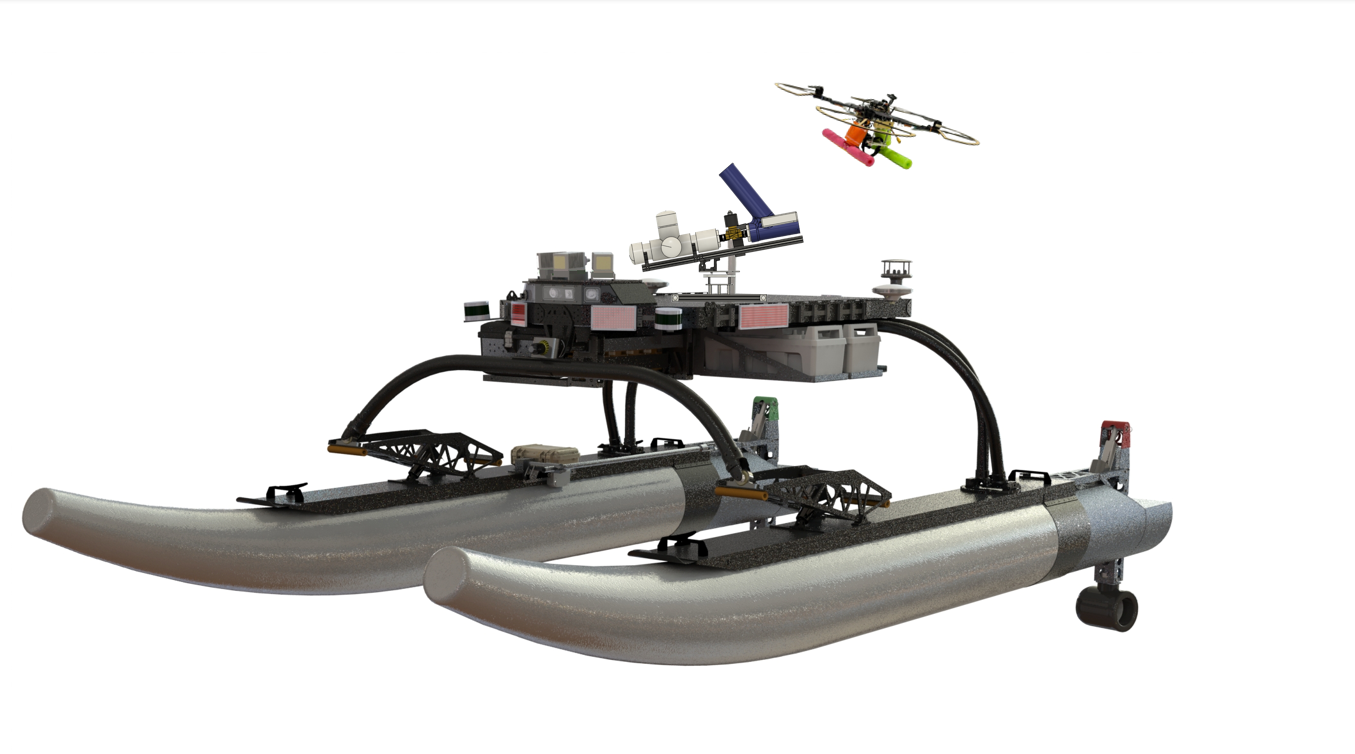
\includegraphics[width=0.8\textwidth]{Images/Minion.png}
\caption{ERAU's \ac{WAMV} Research Vessel Minion as configured for the 2024 Maritime RobotX Challenge.}
\label{fig:minion}
\end{figure}

The sensing configuration used in this research and the 2024 competition is described in Section \ref{perception_geometry}.
% The sensor configuration described in section \ref{perception_geometry} was originally developed by Team Minion for the 2022 and 2024 Maritime RobotX competitions \cite{holland2024, thompson2023}. 
Section~\ref{sensors} presents the technical specifications of Minion's sensor hardware, with particular emphasis on the \ac{LiDAR} and high-definition camera sensors selected for this study.
An overview of the CPU and network infrastructure of the system is provided in section~\ref{Atlas_LAN} as background for the computational requirements of the real-time object detection methods presented in Chapter~\ref{realtime_object_detection}, as well as the challenges relating to the synchronization of sensors in section~\ref{sec:calibration}.
% housed within the forward camera enclosure. Section~\ref{visual_cameras} provides additional discussion regarding visual spectrum sensor selection and characterization. 
Of particular note, the timestamp embedding mechanism described in Section~\ref{time_sync_cam} overcomes network latency issues in the video pipeline to maintain a more precise temporal alignment.
% , essential for rigorous multi-modal sensor fusion analysis.
Finally, section~\ref{sec:sensor_data_dataset} discusses the \ac{ROS} software architecture responsible for recording and processing sensor data.

%%%%%%%%%%%%%%%%%%%%%%%%%%%%%%%%%%%%%%%%%%%%%%%%%%%%%%%%%%%%%%%%%%%%
%%%%%%%%%%%%%%%%%%%%%%%%%%%%%%%%%%%%%%%%%%%%%%%%%%%%%%%%%%%%%%%%%%%%
\section{Perception Geometry} \label{perception_geometry}

Minion is equipped with six \ac{LiDAR} sensors as well as six cameras to perceive her surroundings.
Omnidirectional \ac{LiDAR} coverage is provided by three Velodyne VLP-16 units for situational awareness within the \acp{USV} immediate operating environment.
% \ac{LiDAR} coverage and object detection within the vessel's immediate operating environment.
Three additional forward-scanning Livox Horizon \ac{LiDAR} units generate a dense point cloud ahead of the vessel for object detection and classification at greater distances.
The Livox units are directly mounted to a camera enclosure which houses four high-definition visual-spectrum cameras and two \ac{LWIR} cameras.
The combination of forward-scanning LiDAR and cameras provides a significantly higher fidelity of data within a shared 165-degree \ac{FOV}. % in the direction of travel.
% The camera enclosure design emphasizes modularity and research flexibility.
Figure~\ref{fig:camera_enclosure} illustrates the mounting arrangement of the Livox Horizon LiDAR units and the six cameras within the waterproof enclosure.
Together, these sensors define the operational envelope of the perception system, encompassing a horizontal \ac{FOV} of approximately 160~degrees and an effective detection range of up to 60~meters.

\begin{figure}[htbp]
\centering
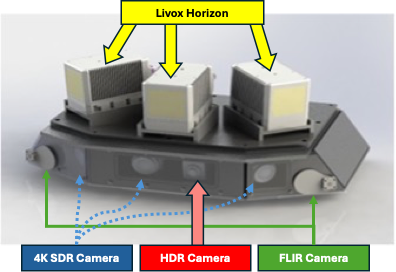
\includegraphics[width=0.6\textwidth]{Images/Camera_enclosure2.png}
\caption{Mounting locations of three Livox Horizon LiDAR units (yellow arrow, top), two LWIR cameras (green, thin, solid arrows), three FLIR 4k cameras (blue, dotted arrows), and a single \ac{HDR} camera  (red arrow, bottom) within the camera enclosure.}
\label{fig:camera_enclosure}
\end{figure}

% While the Velodyne \ac{LiDAR} sensors provide comprehensive 360-degree environmental awareness for navigation and collision avoidance, the three forward-facing Livox Horizon \ac{LiDAR} units mounted to the camera enclosure were selected for their superior point cloud density and ability to facilitate a higher resolution for object detection.
% The three Livox units concentrate sampling density in the forward \ac{FOV}, matching the horizontal coverage of the six cameras.
% Both modalities overlap the \ac{FOV} of their respective individual sensors.
% This sensor arrangement ensures higher density and more uniform point-cloud across the 165-degree forward perception envelope in the case of \ac{LiDAR}, but also makes the system more robust to failure.
% Losing a single sensor will not create a blind spot for either sensing modality in the forward path of motion of the \ac{USV}. 
% Figures~\ref{fig:fov_cam} and ~\ref{fig:fov_LiDAR} show how the horizontal \ac{FOV} for each of these sensors overlaps in the direction of travel.

% Each of these sensors is installed so that the center of their \ac{FOV} is parallel to one of three separate lines of vision.
% The first of these lines is a vector that points down the centerline of the vessel in the forward direction, and sensors in this orientation receive the moniker of \texttt{sensor\_center}.
% The other two lines of vision are rotated 40 degrees counterclockwise and clockwise from the centerline, and sensors in these orientations receive the moniker \texttt{sensor\_port} and \texttt{sensor\_starboard}, respectively.
Each sensor’s optical axis is aligned with one of three predefined sight lines: the vessel's centerline and two axes rotated $\pm 40$ degrees from the center.
% In the case of LiDAR, this sensor arrangement provides a denser point cloud and, in general, means that the loss of signal from any single sensor does not create a blind spot in the forward direction of travel.
For the LiDAR system, this configuration increases point-cloud density in the forward direction and ensures that loss of any single sensor does not produce a blind spot in the forward direction of travel.
% Figure~\ref{fig:fov_combined} shows the camera's \ac{FOV} in \ref{fig:fov_cam}, and the the LiDAR \ac{FOV} in \ref{fig:fov_LiDAR}.
Each of the three Livox Horizon LiDAR units has an 81.7-degree \ac{FOV}, resulting in more than a 40-degree overlap in the \ac{FOV} between \texttt{livox\_center} and both \texttt{livox\_port} and \texttt{livox\_starboard}, and approximately 3 degrees of overlap between \texttt{livox\_port} and \texttt{livox\_starboard} (figure~\ref{fig:fov_LiDAR}).
Three 4K cameras are configured to point in along each of these three sight lines. 
While these cameras are equipped with a Theia-TL410P zoom lens, they are currently set at a fixed zoom level that approximates a 65-degree horizontal \ac{FOV}, which provides a 15-degree overlap in their \ac{FOV} (figure~\ref{fig:fov_cam}).
The two \ac{LWIR} cameras each have a 90-degree \acs{FOV}, and are positioned along the port and starboard vision lines, providing a 10-degree overlap.
Finally, there is a single HDR camera with a 65-degree horizontal \ac{FOV} that points forward.
While the \ac{HDR} camera lacks any of the aforementioned sensor redundancy, its \ac{FOV} aligns with the central 4k camera and was added for research that compared the two center-line mounted cameras \cite{liebergall}.

% related to the dynamic range of the two center-line mounted cameras  and was selected as the primary visual range sensor for this body of work for reasons that are discussed in section~\ref{visual_cameras}.


\begin{figure}[htbp]
\centering
\begin{subfigure}[t]{0.48\textwidth}
    \centering
    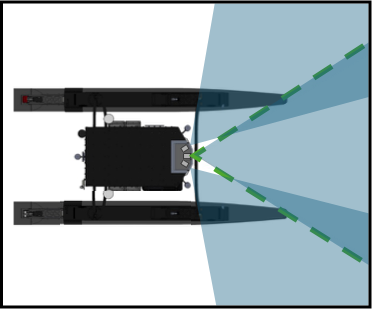
\includegraphics[width=\textwidth]{Images/fov_cam.png}
    \caption{Blue cones represent \ac{FOV} from individual FLIR 4K camera; green dashed lines indicate \ac{FOV} of HDR camera.}
    \label{fig:fov_cam}
\end{subfigure}
\hfill
\begin{subfigure}[t]{0.48\textwidth}
    \centering
    \includegraphics[width=\textwidth]{Images/fov_LiDAR.png}
    \caption{LiDAR horizontal \ac{FOV} overlap.}
    \label{fig:fov_LiDAR}
\end{subfigure}
\caption{Comparative visualization of horizontal \ac{FOV} (FOV) overlap for (a) cameras and (b) LiDAR sensors.}
\label{fig:fov_combined}
\end{figure}

% A Torc Robotics PinPoint \ac{GPS}/\ac{IMU} system is equipped with provides both global time synchronization and platform pose estimation.

% The sensor coordinate frames are organized in a hierarchical transformation tree structure, which is shown in \ref{transform_diagm}.
% The inertial reference frame (\texttt{map}) defines the world-fixed coordinate system.
% The platform reference frame (\texttt{base\_link}) represents the vessel body frame defined by the PinPoint \ac{GPS}/\ac{IMU}.
% The center Livox frame (\texttt{livox\_center}) serves as the primary sensor reference frame, with \texttt{livox\_port} and \texttt{livox\_starboard} both reporting data in the \texttt{livox\_center} reference frame.
% Six camera image frames exist within this tree, and are referenced to the \texttt{livox\_center} frame.
% Intrinsic calibration parameters, including camera-specific matrices and distortion coefficients, along with extrinsic transformation parameters relating sensor frames to each other and to the platform frame, are discussed in \textcolor{red}{Appendix \#}.

% The Livox scan pattern employs a non-repetitive rosette pattern that progressively covers the \ac{FOV} over time rather than repeatedly sampling fixed positions.
% This characteristic enables temporal aggregation to increase effective spatial resolution, particularly beneficial for a moving platform where \ac{GPS}/\ac{IMU} pose data enables motion-compensated point cloud accumulation.

% The dual \ac{LiDAR} architecture serves complementary purposes.
% The Velodyne VLP-16 units provide the omnidirectional awareness required for autonomous navigation, while the Livox Horizon sensors optimize point cloud density specifically within the forward camera \ac{FOV} for fusion research.
% The onboard This configuration enables comparative evaluation of detection performance while maintaining operational navigation capabilities.
% The sensor suite supports the research objectives of comparing detection performance across modalities and evaluating late fusion approaches.
% The following subsections detail individual sensor specifications and selection rationale.

% The primary sensors used for the data collected for this research were from the forward-facing perception module, referred to as the camera enclosure.

%%%%%%%%%%%%%%%%%%%%%%%%%%%%%%%%%%%%%%%%%%%%%%%%%%%%%%%%%%%%%%%%%%%%
%%%%%%%%%%%%%%%%%%%%%%%%%%%%%%%%%%%%%%%%%%%%%%%%%%%%%%%%%%%%%%%%%%%%
\section{Sensors} \label{sensors}

% The Minion platform integrates multiple sensor modalities to support maritime perception research.
% This section details the specifications and characteristics of the visual cameras (Section~\ref{visual_cameras}) \ac{LiDAR} systems (Section~\ref{sensors_LiDAR}), and navigation sensors (Section~\ref{gps_ins}) used in this research.
% , thermal cameras (Section~\ref{thermal_cameras}), and navigation sensors (Section~\ref{gps_ins}) 

%%%%%%%%%%%%%%%%%%%%%%%%%%%%%%%%%%%%%%%%%%%%%%%%%%%%%%%%%%%%%%%%%%%%
\subsection{LiDAR} \label{sensors_LiDAR}

% The Minion platform features six \ac{LiDAR} units providing both omnidirectional environmental awareness and forward-facing high-density perception.
% The \ac{LiDAR} suite is comprised of three Velodyne VLP-16 pucks and three Livox Horizon units.

% Three Velodyne VLP-16 \ac{LiDAR} sensors are positioned at aft-center, with the other two placed at approximately one-third intervals around the vessel at forward-port and forward-starboard, providing complete 360-degree coverage for navigation as well as object detection and avoidance.
% An additional three Livox Horizon solid-state forward-scanning \ac{LiDAR} sensors provide high-density measurements within the forward direction of motion.
Three Velodyne VLP-16 \ac{LiDAR} sensors are installed around the vessel to provide omnidirectional situational awareness. 
One unit is mounted near the aft-center position, and the other two are positioned at approximately one-third intervals around the forward-port and forward-starboard quadrants. 
Together, these sensors deliver nearly continuous 360° coverage for navigation and obstacle avoidance.

Each VLP-16 employs 16 lasers arranged in a vertical array that scans 16 distinct points elevation over its 30-degree vertical \ac{FOV} continuously over the 360-degree azimuth, producing approximately 300,000 \ac{pps} in single-return mode. 
The units are installed with a downward declination of approximately 5 degrees from the plane of the \ac{USV} deck to minimize blind-spots near the vessel's waterline.
As a result, one-half to one-third of their scanning azimuth is well above the horizon or pointing directly into the vessel and is discarded, drastically reducing the number of points each unit can publish.

% Both of these units are capable of approximately 1.4 million measurements per second.
% For an equivalent 80-degree horizontal FOV, the Velodyne’s effective $317,700 \text{ pts/sec}$ represents $\approx 22 \%$ of the overlapping \ac{FOV} of the Livox unit’s output.
% % While each Velodyne VLP-16 unit is capable of producing 300k \ac{pps} compared to the Livox unit's 280k, their 360-degree scanning pattern means that only 
% The principal distinction between them lies in their underlying scanning architectures and sampling density, which directly influences perception fidelity.
% The Velodyne VLP-16 LiDAR scans 16 discrete points spanning a 30-degree vertical \ac{FOV} emanating from the azimuthal plane of the device in a 360-degree horizontal \ac{FOV}that repeats identically with each rotation. 
% The points generated span the 360
% % To minimize blind spots near the base of Minion, each of the Velodyne units is mounted at a 15-degree declination from the vessel's deck plane, resulting in 
% These rings are notF
% % For vessels moving at typical speeds (2-5 m/s), platform displacement between rotations remains small relative to object size, resulting in near-perfect overlap of consecutive scans.
% At typical vessel speeds between $2 \text{to} 5 m/s$, successive Velodyne rotations overlap almost perfectly, causing sparse sampling of small or distant targets.
% % This means that small to medium-sized objects may not even be detected when at large distances from the sensor, as illustrated in Figure \ref{fig:LiDAR_scan_compare}.
% Consequently, small or distant targets may be undersampled or entirely missed in sequential Velodyne frames (Figure \ref{fig:LiDAR_scan_compare}).

In contrast, the three Livox Horizon solid-state \ac{LiDAR} units concentrate their scanning pattern within an $81.7 \times 25.1$ degree \ac{FOV}, generating up to 280,000 \ac{pps}. 
Although the nominal point rates are comparable, the Livox pattern can return $100 \%$ of its concentrated \ac{FOV} data. 
This higher spatial sampling density enables detection and classification of objects that may be smaller or further from the sensor.
A direct comparison of the discrepancy between the Velodyne and Livox scan patterns and point density is provided in Figure \ref{fig:LiDAR_scan_compare}.
The top-right image shows the dense point cloud of the Livox devices.
The light tower in the foreground and the large dock structure in the background can be seen in the camera view (left) and are both well defined in the red point cloud.
Two small buoys are also distinctly visible between the two structures.
In comparison, the point cloud returned by the Velodyne devices is shown in the bottom-right. 
The general form of the light tower can be seen; however, there are very few points returned from the large dock structure in the background, and the round buoys are undetected.

% The forward-scanning Livox devices operate differently, tracing a non-repetitive pattern across the \ac{FOV}.
% Two orthogonal mirrors oscillate at slightly different frequencies to cause the laser beam to trace a path that progressively fills the \ac{FOV} without repetition as shown in Figure ~\ref{fig:livox_scan_pattern}.

\begin{figure}[htbp]
\centering
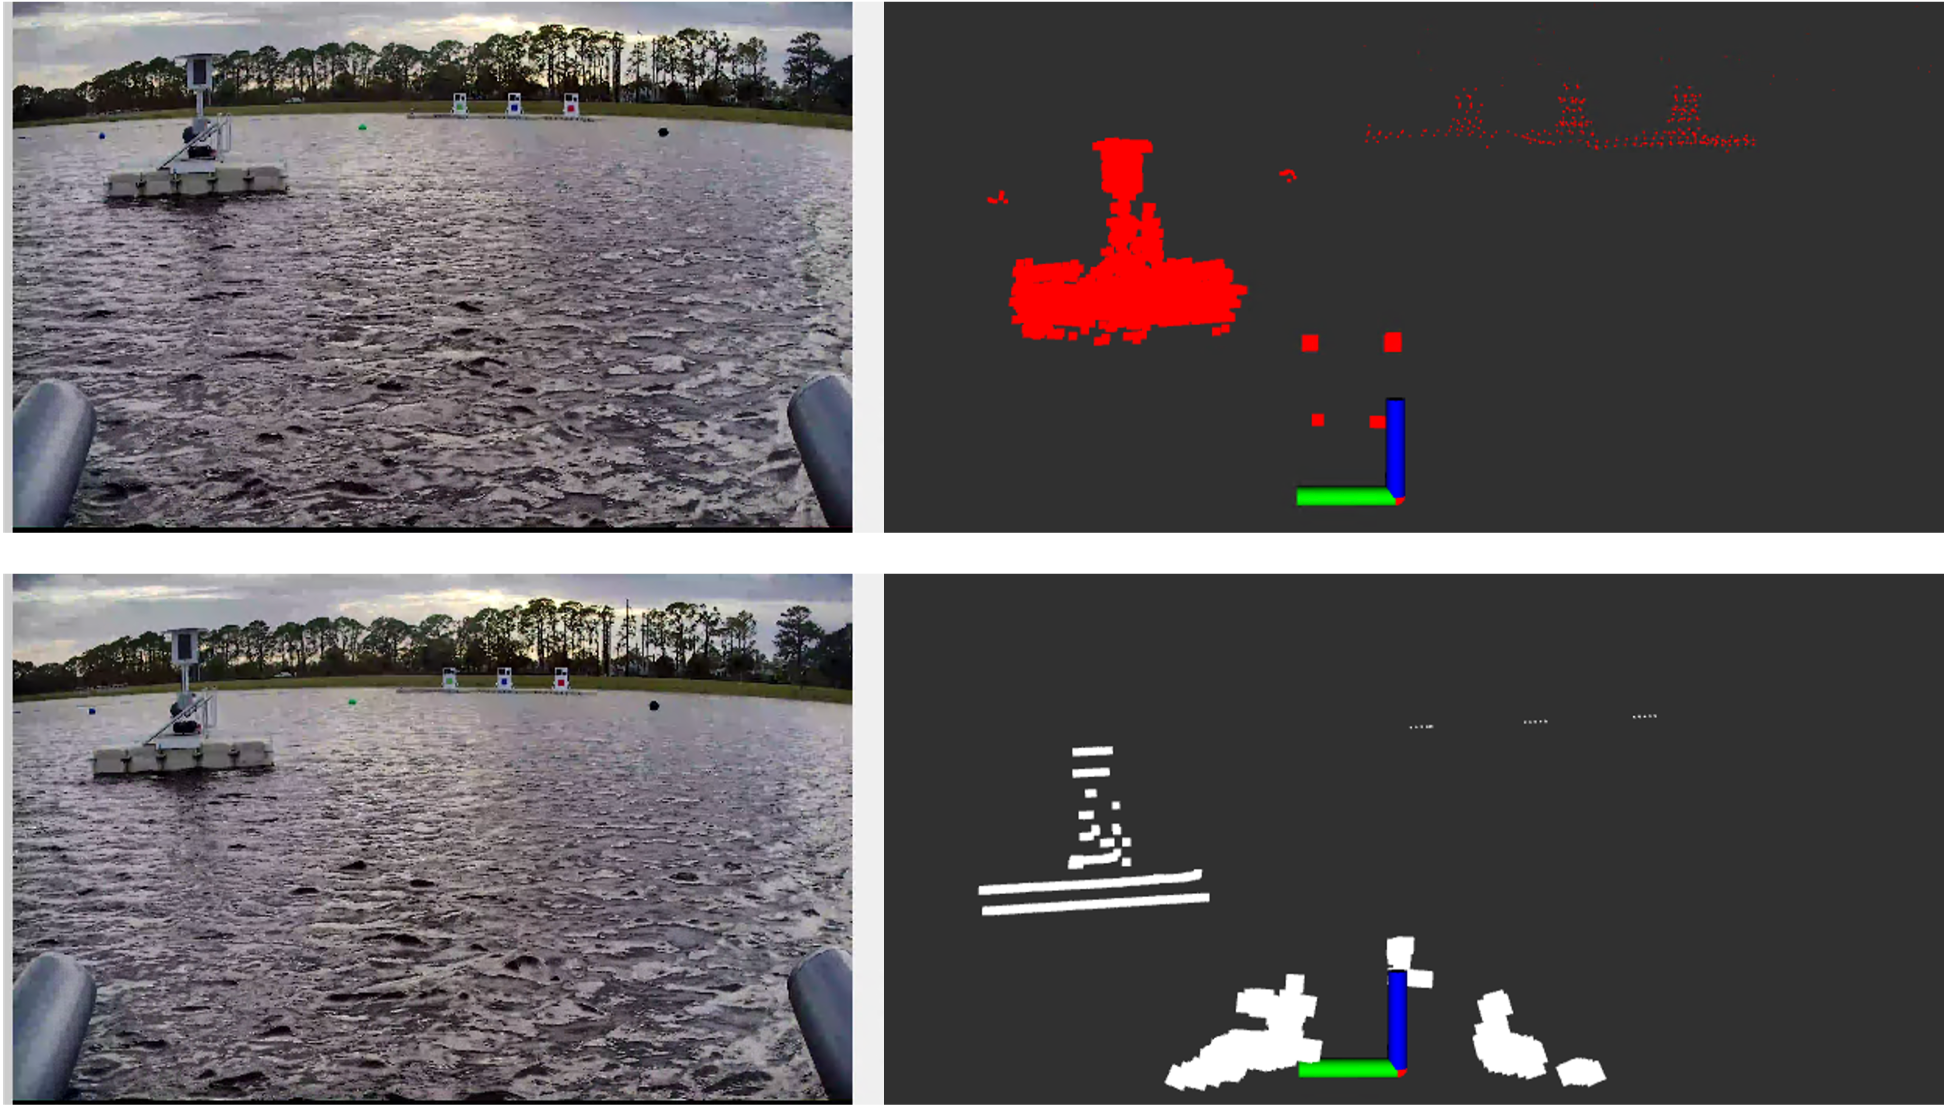
\includegraphics[width=0.8\textwidth]{Images/LiDAR_compare.png}
\caption{A comparison of LiDAR returns from the Livox units (top-right, red) and Velodyne units (bottom-right, white) to the respective HDR camera view (top-left and bottom-left). LiDAR points are viewed from third-person point of view in RVIZ. Green and Blue axes (top-right, top-bottom) represent the origin of the USV frame of reference.}
\label{fig:LiDAR_scan_compare}
\end{figure}

% The superior point density of the overlapping forward-scanning  LiDAR is critical for the real-time object detection method that is discussed in \textcolor{red}{Section \#}.
% The overlapping forward-scanning LiDAR provides the spatial density required for the real-time object-detection framework described in Section \ref{gbcache}.
% For this reason, the research presented in this work exclusively utilizes LiDAR data from the Livox Horizon sensors.

Consequently, the research presented in this work relies exclusively on LiDAR data from the forward-scanning Livox Horizon sensors, whose concentrated and non-repetitive coverage provides the spatial resolution required for the real-time object-detection framework described in Section \ref{gbcache}.
        %%%%%%%%%%%%%%%%%%%%%%%%%%%%%%%%%%%%%%%%%%%%%%%%%%%%%%%%%%%%
\subsubsection{Livox Horizon} \label{sensors_livox}

% Each Livox Horizon employs two orthogonal mirrors operating at different frequencies to trace a complex Lissajous-like path that progressively fills the $81.7 \times 25.1$-degree (horizontal × vertical) \ac{FOV}, as illustrated in Figure~\ref{fig:livox_scan_pattern}. 
% The three Livox units are mounted with 40 degrees of horizontal separation, overlapping each other \ac{FOV} by $\approx 50\%$, making the system robust to failure of any single unit, as well as effectively doubling the rate of sampled points and distributing them more evenly across the center device's \ac{FOV}. 
Each Livox Horizon uses dual orthogonal mirrors oscillating at slightly different frequencies to generate a non-repetitive Lissajous-like scan pattern over its $81.7 \times 25.1$ degree \ac{FOV}. 
Overlapping these sensors by roughly $50 \%$ effectively doubles the point density along the center-line path under nominal operation, and maintains coverage under single-unit failure.
Table~\ref{table:livox_horizon_specs} presents detailed hardware specifications for the Livox Horizon.

% The rosette scan pattern is provided in \ref{fig:livox_scan_pattern}, and table \ref{table:livox_horizon_specs} presents the Livox Horizon specifications.

\begin{figure}[htbp]
\centering
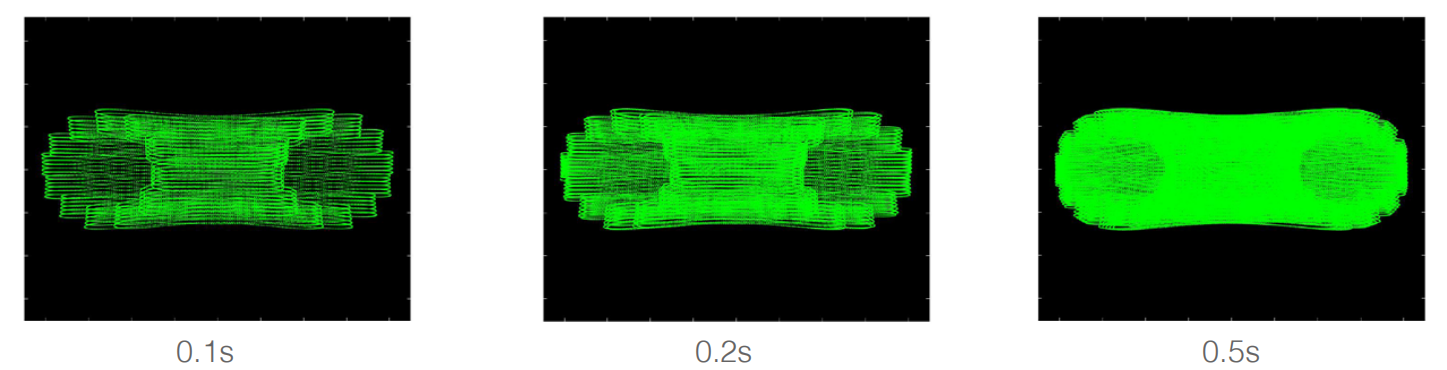
\includegraphics[width=0.8\textwidth]{Images/Livox_1.png}
\caption{Accumulation of points with the Livox Horizon's non-repetitive scan pattern, from 0.1 to 0.5 seconds  \cite{livox_manual}.}
\label{fig:livox_scan_pattern}
\end{figure}

Each device is capable of returning up to $4.8 \times 10^5$ \ac{pps} in dual return mode, with each return consisting of position coordinates (x, y, z), target reflectivity, and timestamp.
This operational mode returns two data points for each laser emission and is useful for situations where the sensor scans semi-permeable objects such as windows, thick tree canopies, or water.
% Instead, each device is operated in single-return mode for two reasons.
% The first is a consideration of available network bandwidth.
Each sensor operates in single-return mode, primarily to reduce network load.
A conservative estimate of 16 bytes per point results in $\approx 23 \text{ Mbps}$ which would quickly overwhelm the \ac{USV}'s network.
% Luckily, the 905 nm near-infrared wavelength of the emitted laser experiences strong absorption by water. 
However, The $905 nm$ near-infrared emission is strongly absorbed by water, effectively suppressing subsurface returns.
This means that only points which are reflected by the water surface are returned with an intensity greater than zero, making it straight forward to filter out points in the ground plane.

\begin{table}[htpb]
\centering
\begin{tabular}{ll}
\hline
\multicolumn{2}{c}{Livox Horizon}\\
\hline
% \textbf{Parameter} & \textbf{Value} \\
\hline
Model & Livox Horizon \\
Horizontal Field of View & 81.7 degree \\
Vertical Field of View & 25.1 degree \\
Range & 260 m @ 80\% reflectivity \\
Point Rate (Single Return) & 240,000 pts/sec \\
Point Rate (Dual Return) & 480,000 pts/sec \\
Range Precision & ±2 cm \\
Wavelength & 905 nm \\
Scan Pattern & Non-repetitive rosette \\
Interface & Ethernet \\
Operating Frequency & 100 Hz \\
\hline
\end{tabular}
\caption{LiDAR Specifications}
\label{table:livox_horizon_specs}
\end{table}

%%%%%%%%%%%%%%%%%%%%%%%%%%%%%%%%%%%%%%%%%%%%%%%%%%%%%%%%%%%%%%%%%%%%
\subsection{Visible Spectrum Cameras} \label{visual_cameras}

% \textcolor{red}{Expand this entire discussion}
% The visible spectrum camera suite on the Minion platform is designed to balance two factors that are particularly important for maritime perception: imaging resolution and dynamic range.

For computer vision and perception tasks, system performance is directly influenced by the quality of the visual input.
The fidelity of an image is determined by a camera's hardware and integrated software; therefore, camera selection is a critical design consideration in any vision-based system. 
Sensor size and lens characteristics determine the spatial detail captured, while shutter speed, exposure, and onboard processing influence brightness, contrast, and color balance. 
The visible-spectrum cameras housed within the camera enclosure were selected to balance image resolution and dynamic range, two essential factors for reliable maritime perception.
A brief discussion of both of these metrics is presented here to justify utilizing data acquired from the \ac{HDR} camera for this research.

\subsubsection{Image Resolution}
Camera resolution determines the ability to resolve small targets at a distance.
% , and appropriate imaging sensors and lenses can be selected by determining the maximum distance and minimum size at which objects need to be resolved.
% Camera resolution dictates the minimum discernible target size at range; lens and sensor parameters are therefore chosen to meet specified detection distances.
% Camera resolution governs the minimum resolvable target size; lens and sensor parameters are thus selected to ensure detection at required ranges.
To ensure adequate perception across the operational envelope, cameras must resolve objects to a required minimum resolution when the object is at the maximum detection range.
% The resolution of an object in the image frame can be determined if the object's width $\mathit{l}$ and distance from the camera $d$ are knownwith
The relationship between an object's physical width $\mathit{w}_{obj}$ and pixel width within an image $\mathit{w}_{\text{px}}$ is given by
% Provided a maximum detection range $d$ and the width of the smallest object to be detected $W$, the camera's focal length and resolution requirements can be determined by assuming a pinhole-camera model \cite{matlab_calibration}, can be derived as:
% we can determine the necessary optical focal length and resolution for the sensor.
% For an object of physical width $W$ at distance $d$, its width in the image frame $w_{\text{px}}$ is approximated by

\begin{equation}
\mathit{w}_{\text{px}} = f \; \frac{N_x}{S_w}\frac{\mathit{w}_{obj}}{d}
\end{equation}

% where $\mathit{l}_{\text{px}}$ is the pixel width of an object in the image frame, 
where $f$ is the \ac{EFL} of the camera and lens, $N_x$ is the horizontal image resolution in pixels, and $S_w$ is the width of the image sensor.
% This equation is used for sensor selection by determining the minimum resolution required for the smallest object to be detected at the maximum detection range.
This equation can be used to determine camera requirements if the true size of the imaged objects is known, or to determine a reasonable expectation of object resolution if the camera values are known.
This relationship is also critical for determining the distortion present in each camera/lens system, detailed further in section~\ref{spatial_calibration}.

Defining the requirement for the minimum resolution of an object in the image frame requires an understanding of the object detection method used with visual cameras, as well as the objects being detected. both of which will be discussed in greater detail in sections ~\ref{sec:sensor_data_dataset} and ~\ref{yolo}, respectively.
% For now, it is sufficient to know that the smallest object we wish to detect is $0.3683$ meters wide at a distance of 60 meters.
% , and that we have optical and digital resolution requirements to consider.
This image detection architecture is discussed in section ~\ref{yolo}.
For camera selection, it is sufficient to know that this method scales down each input image to a resolution of $640 \times 640$ pixels for processing efficiency.
This should be considered when defining the minimum pixel density of a camera's sensor, as it alters our prior equation slightly.

\begin{equation}
\mathit{w}'_{\text{px}} = f \; \frac{640 \text{px}}{S_w}\frac{\mathit{w}_{obj}}{d}
\end{equation}
% This means that an image captured at $4000 \times 3000$ pixels is reduced to $650 \times 487$ pixels, which is $16.25\%$ of its original size.
% As an example, if the text on waterway signage 60 meters away is legible at a resolution of 100 pixels wide in a 1,000 $\times$ 1,000 pixel image, it would need a resolution of 162 pixels to meet the additional requirements imposed by the image detection algorithm.
Each camera within the enclosure was selected using these metrics, and object information based on the obstacles commonly associated with the RobotX Maritime Challenge. %, in addition to other contemporaneous research \cite{thompson2023} \textcolor{red}{(check scholarly commons)}.

% \textcolor{red}{add back: ?}
Given that the smallest object we wish to detect is $0.3683$ meters wide at a distance of 60 meters.
The two visual spectrum camera models within the camera enclosure have a similar focal length, and resolutions of $4000 \times 3000$ px and $2880 \times 1860$ px. Examining the camera with the smaller horizontal resolution of 1880 px (which has a sensor width of $S_{w} = 8.64$ mm), we obtain the width of our object in the image frame as
% meet this requirement; the object detection method used will impose a secondary constraint.
\begin{equation*}
\begin{split}
    \mathit{w}_{\text{px}} & = 8\;\text{mm} \cdot \frac{2880\;\text{px}}{8.64\;\text{mm}} \cdot \frac{0.3683\;\text{m}}{60\;\text{m}}\\
     & = 16.36 \approx 16 \;\text{px}
\end{split}
\end{equation*}

With the additional scaling required by the visual object detection method, the minimum width of our object becomes 
\begin{equation*}
\begin{split}
    \mathit{w}'_{\text{px}} & = 16\;\text{px} \cdot \frac{640\;\text{px}}{2880\;\text{px}} \\
     & = 3.\overline{55} \approx 3 \;\text{px}
\end{split}
\end{equation*}

Figure \ref{fig:A2_multi_res} shows our smallest object, Polyform A2 round buoy, at a selection of resolutions, and is still recognizable at a resolution of 16 pixels wide. %, and becomes less defined at lower resolutions. 
This operation is repeated to predict the width of the object in the image frame at a range of distances up to our maximum of 60 meters, and the results are provided in Table \ref{table:buoy_res}.
From this information, the buoy will be easily recognizable at any range by visual inspection, but will become much less defined when the image is scaled down for the visual object detection method.
As we will discuss in section \ref{yolo}, this method may struggle to detect this size buoy at distances greater than 20 meters.

\begin{table}[htpb]
\centering
\begin{tabular}{c|c|c}
\hline
\multicolumn{3}{c}{Polyform A2 Buoy Resolution at Range}\\
\hline
% \textbf{Parameter} & \textbf{Value} \\
\hline
Object Distance & Image Frame Width & With Detection \\
\hline
10 m & 98 px & 21 px \\
20 m & 49 px & 10 px \\
30 m & 32 px & 7 px \\
40 m & 24 px & 5 px \\
50 m & 19 px & 4 px \\
60 m & 16 px & 3 px \\
\hline
\end{tabular}
\caption{The predicted resolution of a $\mathit{l} = 0.3683$ meter wide object within the Loepard Imaging HDR camera's image frame at multiple distances.}
\label{table:buoy_res}
\end{table}

\begin{figure}[htbp]
\centering
\begin{subfigure}[t]{0.245\textwidth}
    \centering
    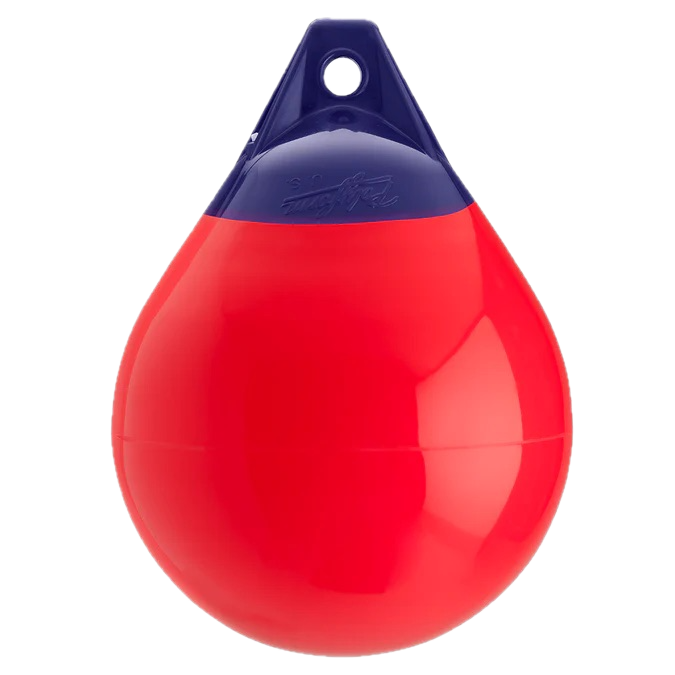
\includegraphics[width=\textwidth]{Images/A2.png}
    \caption{\raggedright{Polyform A2 Buoy}}
    \label{fig:A2}
\end{subfigure}
\hfill
\begin{subfigure}[t]{0.245\textwidth}
    \centering
    
\includegraphics[width=\textwidth]{Images/A2_16px.png}
    \caption{
    16 pixel width,\\  
    % $\approx$ 60 m with HDR
    }
    \label{fig:A2_16px}
\end{subfigure}
\hfill
\begin{subfigure}[t]{0.245\textwidth}
    \centering
    
\includegraphics[width=\textwidth]{Images/A2_6px.png}
    \caption{
    6 pixel width,\\  
    % $\approx$ 40 m with HDR \\ 
    % \& object detection.
    }
    \label{fig:A2_6px}
\end{subfigure}
\hfill
\begin{subfigure}[t]{0.245\textwidth}
    \centering
    
\includegraphics[width=\textwidth]{Images/A2_3px.png}
    \caption{
    3 pixel width,\\  
    % $\approx$ 60 m with HDR \\ 
    % \& object detection.
    }
    \label{fig:A2_3px}
\end{subfigure}
\caption{Polyform A2 Buoy (a), visualized at 16 pixels (b), 6 pixels (c), and 3 pixels wide (d).}
\label{fig:A2_multi_res}
\end{figure}




% The dynamic range of an imaging sensor refers to the range of signal intensities it can detect, and can be as critical as image resolution when selecting camera sensors.
\subsubsection{Dynamic Range}
Dynamic range describes the ratio between the brightest and darkest signal levels a camera sensor can record.
Light levels that exceed the camera sensor's range cause the image to appear white or "blown-out", while light levels that are too low will appear darker, with detail being indistinguishable from noise.
% Dynamic range—the span of detectable signal intensities—is equally critical to sensor selection as spatial resolution.
\acp{USV} and \acp{AGS} routinely operate in environments where bright sky reflections and deep shadows are common, often within the same scene.
Therefore, selecting a camera with insufficient dynamic range may lead to washed-out highlights or lost detail in shadows.

Dynamic range, expressed in dB, is given by
\begin{equation}
 \text{Dynamic Range (dB)} = 20 \log{\left( \frac{N_{sat}}{N_{noise}}\right) }
\end{equation}
where $N_{sat}/N_{noise}$ is the ratio of the saturation to the minimum signal a camera sensor can detect above background noise.
% Higher dynamic range can be achieved through software by combining sequential multi-exposure images, or through a digital overlap \ac{HDR} (DOL-HDR) architecture with in-pixel dual conversion gain.
% Sequential multi-exposure \ac{HDR}, which stacks separate frames and is prone to ghosting or blurring, therefore 
% DOL-\ac{HDR} is preferred when precise synchronization of the imagery is required, such as sensor fusion.
% Because maritime environments routinely present both bright sky reflections and deep shadows in the same scene, dynamic range is as critical as resolution when selecting cameras for perception tasks. 
High-dynamic-range (HDR) imaging can be achieved in two primary ways. 
The first is sequential multi-exposure \ac{HDR}, in which multiple frames captured at different exposure settings are combined to extend the tonal range \cite{Reinhard2010}. An example is provided in Figure \ref{fig:hdr_example}.



While effective for static scenes, this approach introduces motion-related artifacts such as ghosting and motion-blur as the relative velocity increases between the sensor and objects within the frame.
The second method uses an in-sensor technique called dual-conversion gain (DCG) that combines multiple light exposure levels within a single frame of exposure. 
% \textcolor{red}{Coyle: It isn't short and long exposure, but changing the size of the exposure pixel to capture more/less light from my understanding. This is why it doesn't motion blur} By capturing short and long exposure data within a single frame, this method avoids the distortion of multi-exposure \ac{HDR}.
The two visible sensing technologies considered for this research are described below.

\begin{figure}[htbp]
    \centering
    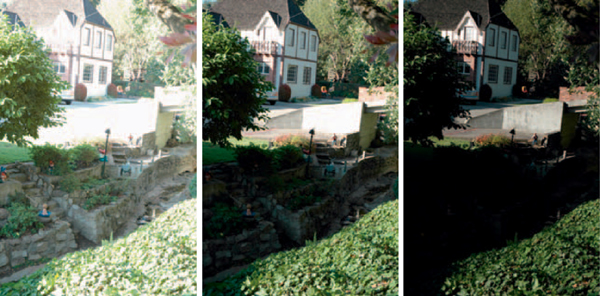
\includegraphics[width=0.65\linewidth]{Images/hdr_example.png}
    \caption{An example of multi-exposure HDR frame-stacking \cite{Reinhard2010}.}
    \label{fig:hdr_example}
\end{figure}
%%%%%%%%%%%%%%%%%%%%%%%%%%%%%%%%%%%%%%%%%%%%%%%%%%%%%%%%%%%%%%%%%%%%
\subsubsection{FLIR Blackfly S 4K Cameras} \label{sensors_FLIR}

% Three FLIR Blackfly S 4K visible-light cameras, arranged to provide a combined 165 degrees of forward-facing coverage through overlapping 65-degree lenses.  
Three FLIR Blackfly S 4K cameras are aligned to the port, center, and starboard sight-lines described in section \ref{perception_geometry} to provide a combined 165-degree horizontal \ac{FOV}.
In addition to redundancy, this configuration avoids additional spherical distortion within the image that would be required to cover the same \ac{FOV} with fewer cameras.
% Each camera is paired with a Theia TL410P zoom lens with an \ac{EFL} of \textcolor{red}{???} and an image resolution of $4096 \times 4096$, ensuring that objects remain adequately resolved across the vessel's perception envelope.  
Each FLIR Blackfly has a resolution of 4096 $\times$ 4096 pixel resolution and is paired with a Theia TL410P zoom lens at a fixed \ac{EFL} $\approx$ 8 mm.
% This sensor dimension and \ac{EFL} exceeds the pixel density required to ensure object resolution across the operational envelope.


\begin{table}[htbp]
\centering
\begin{tabular}{ll}
\hline
\multicolumn{2}{c}{FLIR 4K SDR Camera}\\
% HDR & Camera\\
\hline
% \textbf{Parameter} & \textbf{Value} \\
\hline
\multicolumn{2}{c}{Camera Sensor}\\
\hline
FLIR & Blackfly S 120S4C \\
% Image Sensor & Sony IMX490 \\
% Pixel Size & $3.0 \times 3.0 \mu m$ \\
Horizontal Resolution & 4000 pixels \\
Vertical Resolution & 3000 pixels \\
Aspect Ratio & 1.33:1 \\
Maximum Frame Rate & 31 fps \\
Dynamic Range & 69.4 dB \\
\multicolumn{2}{c}{Camera Lens}\\
\hline
Theia & TL410P\\
% Aperture F/\# & $2.0$ \\
Horizontal \Ac{FOV} & 65-degrees\\
Lens \Ac{EFL} & approx. 8 mm\\
% Vertical Field of View & 37 degrees \\
\hline
\end{tabular}
\caption{FLIR 4K SDR Camera Specifications}
\label{table:SDR_camera_specs}
\end{table}

The Blackfly S sensor captures video at 31 \ac{fps} and achieves a dynamic range of 69.4 dB, which is within the \ac{SDR}.
% This corresponds to a span of a few thousand-to-one between the darkest detectable signal and the brightest non-saturating signal.  
% The cameras capture 31 \ac{FPS} at a resolution of 4096 $\times$ 2160 pixels.
% \textcolor{red}{Add discussion of pixel density sensor selection in the context of the requirement to resolve specific objects at a minimum resolution at a maximum specific distance. This will require equations.}

%%%%%%%%%%%%%%%%%%%%%%%%%%%%%%%%%%%%%%%%%%%%%%%%%%%%%%%%%%%%%%%%%%%%
\subsubsection{Leopard Imaging HDR Camera} \label{sensors_HDR}

% A Leopard Imaging LI-USB30-IMX490-GW5400-GMSL2-065H camera, based on Sony’s IMX490 automotive-grade \ac{HDR} sensor, provides 65-degree of forward \ac{FOV}.  
The Leopard Imaging camera provides a 65-degree forward \ac{FOV} using Sony’s automotive-grade IMX490 sensor with 120 dB of dynamic range.
The \ac{HDR} is achieved via Sony’s \ac{DOL-HDR} architecture, which combines large and small photodiodes within each pixel on the sensor.
Each size of sub-pixels experience a different photon flux during each frame of exposure, and each output is read at both high and low conversion gains.
This method yields 4 measurements of light intensity within each captured frame, eliminating motion artifacts and enabling precise temporal alignment for sensor fusion.
Table \ref{table:hdr_camera_specs} provides detailed specifications for the HDR camera, which delivers a resolution of $2880 \times 1860$ pixels at 25 frames per second with a dynamic range of 120~dB
% Sony’s \ac{DOL-HDR} architecture exposes both sub-pixels (SP1 and SP2) simultaneously but reads them sequentially at different conversion gains to capture multiple brightness levels within a single frame.
% It utilizes two sizes of sensing pixels, one large and one small, which receive different flux of of photons per exposure,  within a single frame period. \textcolor{red}{Coyle: use same terminology as where you described this earlier.}
.%, extending the span of detectable light intensity to nearly one million-to-one.  

% The IMX490 accomplishes this \ac{HDR} using a digital overlap \ac{HDR} (DOL-HDR) architecture with in-pixel dual conversion gain.  

% This method captures multiple effective exposures within a single frame period, producing simultaneous multi-gain readouts from the same scene.  
% This architecture produces simultaneous multi-gain readouts without sequential stacking, 

\begin{table}[htpb]
\centering
\begin{tabular}{ll}
\hline
\multicolumn{2}{c}{Leopard Imaging HDR Camera}\\
% HDR & Camera\\
\hline
% \textbf{Parameter} & \textbf{Value} \\
\hline
% Make & Leopard Imaging \\
Leopard Imaging & LI-IMX490-GW5400-GMSL2-065H \\
Image Sensor & Sony IMX490 \\
Pixel Size & 3.0 $\times$ 3.0 $\mu$m \\
Horizontal Resolution & 2880 pixels \\
Vertical Resolution & 1860 pixels \\
Aspect Ratio & 1.55:1 \\
Maximum Frame Rate & 25 fps \\
Dynamic Range & 120 dB \\
Aperture F/\# & $2.0$ \\
Horizontal \Ac{FOV} & 65-degrees \\ %(H), 37-degrees (V) \\
% Vertical Field of View & 37 degrees \\
Lens \Ac{EFL} & 7.9 mm\\
\hline
\end{tabular}
\caption{Leopard Imaging HDR Camera Specifications}
\label{table:hdr_camera_specs}
\end{table}


%%%%%%%%%%%%%%%%%%%%%%%%%%%%%%%%%%%%%%%%%%%%%%%%%%%%%%%%%%%%%%%%%%%%
\subsubsection{Camera Selection} \label{camera_selection}

The combination of image resolution and \ac{EFL} of both cameras exceeds the pixel density required to ensure object resolution across the operational envelope.
\textcolor{red}{Coyle: which you never told me}
FLIR Blackfly S 4K cameras exceed the resolution requirements, but their limited dynamic range of 69.4~dB makes them prone to over-exposure and reduced contrast under extreme lighting conditions. 
% They support an effective dynamic range of 69.4~dB, which corresponds to a span of just a few thousand-to-one between the darkest detectable signal and the brightest non-saturating signal. 
% As a result, the cameras are prone to over-exposure in high-brightness maritime conditions, particularly when imaging reflective water surfaces or bright sky backgrounds, leading to loss of highlight detail and reduced contrast. 

\begin{figure}[htbp]
\centering
\makebox[\textwidth][c]{%
    \begin{subfigure}[t]{0.35\textwidth}
        \centering
        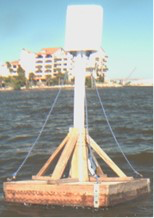
\includegraphics[width=\textwidth]{Images/SDR_bright.png}
        \caption{SDR visual camera (5 MP)}
        \label{fig:SDR_bright}
    \end{subfigure}
    \hspace{2em} % horizontal spacing between them
    \begin{subfigure}[t]{0.378\textwidth}
        \centering
        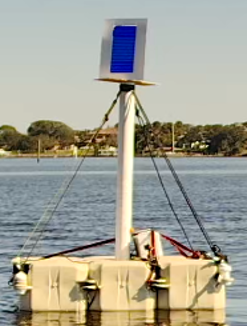
\includegraphics[width=\textwidth]{Images/HDR_bright.png}
        \caption{HDR visual camera (5 MP)}
        \label{fig:HDR_bright}
    \end{subfigure}%
}
\caption{\textcolor{red}{place-holder image – A visual comparison of the \ac{SDR} FLIR 4k camera (left) and the \ac{HDR} Leopard Imaging camera (right) in low-light conditions.}}
\label{fig:HDR_compare}
\end{figure}

In contrast, the Leopard Imaging \ac{HDR} camera offers slightly lower image resolution at a comparable effective focal length but provides substantially greater dynamic range.
% enabling detail preservation across bright and shaded regions within the same frame.  
This wider dynamic range enables more consistent color fidelity and image contrast under suboptimal lighting conditions, as illustrated in Figure~\ref{fig:HDR_compare}.

% Many tasks in the 2024 Maritime RobotX Challenge required \acp{USV} to accurately distinguish object colors as part of their operational decision-making.
This capability motivated the selection of the \ac{HDR} camera as Minion's primary visual camera sensor for the 2024 Maritime RobotX Challenge, which included several tasks that required \acp{USV} to accurately identify object colors in order to make operational decisions.
\textcolor{blue}{Check these results again}\textcolor{blue}{A comparative study by Liebergall et al.~\cite{liebergall} further supported this decision, as preliminary results indicated improved object detection results with data from the \ac{HDR} over the FLIR \ac{SDR} camera.}
Because the data collected during that competition formed the foundation of this dissertation, the Leopard Imaging \ac{HDR} camera, the primary visual spectrum sensor, was selected for all research presented in this paper.

% For these reasons, the \ac{HDR} camera was designated as the primary forward-facing visual spectrum sensor for the \ac{LiDAR}-camera fusion research presented in this paper.  




%%%%%%%%%%%%%%%%%%%%%%%%%%%%%%%%%%%%%%%%%%%%%%%%%%%%%%%%%%%%%%%%%%%%
%%%%%%%%%%%%%%%%%%%%%%%%%%%%%%%%%%%%%%%%%%%%%%%%%%%%%%%%%%%%%%%%%%%%

\subsection{PinPoint GPS/INS} \label{sensors_GPS}

% The Minion platform features a PinPoint \ac{GPS}/\ac{INS} equipped with dual-antennae for orientation and differential corrections for millimeter precision geolocation.
% The sensor performs two critical functions for the \ac{USV}: tracking vessel position and orientation, and precise global time for sensor synchronization.
% The \ac{GPS} receiver functions as the master clock for the entire synchronization hierarchy described in ~\ref{time_sync}, while the integrated \ac{IMU} enables high-rate pose updates between \ac{GPS} fixes.

The Minion \ac{USV} employs a Torc Robotics Pinpoint \ac{GPS}/\ac{INS} unit for both global positioning and inertial navigation capabilities.
This device integrates a differential-corrected \ac{GPS} receiver with a multi-axis \ac{IMU} and dual antenna, providing precise position, velocity, and orientation data for the autonomous platform.
The \ac{GPS} receiver is configured to operate at an update rate of five Hz, while the integrated \ac{IMU} provides high-frequency inertial measurements at 105.4 Hz.
The Pinpoint unit delivers timing accuracy on the order of 10-100 nanoseconds for \ac{GPS}-disciplined time signals, which is a critical function for multi-sensor synchronization discussed in Section~\ref{time_sync}.


%%%%%%%%%%%%%%%%%%%%%%%%%%%%%%%%%%%%%%%%%%%%%%%%%%%%%%%%%%%%%%%%%%%%
%%%%%%%%%%%%%%%%%%%%%%%%%%%%%%%%%%%%%%%%%%%%%%%%%%%%%%%%%%%%%%%%%%%%
\section{Compute Hardware and Network} \label{Atlas_LAN}

Minion distributes processing tasks across multiple computing nodes to achieve real-time performance and robust system operation.
The computing infrastructure consists an embedded computer integrated with the camera sensors for video encoding and streaming, and twin computers serving as the primary processing platforms, with a \ac{GbE} \ac{LAN} connecting all systems and sensors. 
% This architecture distributes computational workloads according to sensor proximity and processing requirements while maintaining centralized coordination through the Robot Operating System middleware. 
The following subsections detail the hardware specifications, system architecture, and network infrastructure that enable real-time multi-modal perception for maritime object detection and sensor fusion.

%%%%%%%%%%%%%%%%%%%%%%%%%%%%%%%%%%%%%%%%%%%%%%%%%%%%%%%%%%%%%%%%%%%%
\subsection{Camera Enclosure} \label{subsec:camera_enclosure}

% # Camera Enclosure Computing Platform

The camera enclosure serves as the integrated perception module for the vessel, and was designed as a self-contained sensor and computing subsystem that can operate independently on any maritime or ground vehicle. 
Integrated into this subsystem is a NVIDIA Jetson AGX Xavier, a compact and capable PC designed for video processing, as well as other computer vision applications.
Key hardware specifications are provided in table \ref{table:Xavier_hardware}.

Its 8-core ARM processor provides ample computational capacity for handling multiple video pipelines, network protocols, and system-level services, while the integrated 512-core Volta GPU performs hardware-accelerated video encoding required for concurrent high-resolution streams.  
A unified memory architecture shares 32 GB between the CPU and GPU and supports a memory bandwidth of 136.5 GBps, which minimizes latency and improves overall pipeline efficiency.

Each video feed follows a two-branch processing pipeline before being transmitted to Atlas, detailed in section \ref{time_sync_cam}.

Raw video frames are received via USB 3.0, parsed by custom software, and then split into two processing branches. 
One branch is compressed and saved locally to the Jetson's internal storage, while the other branch is down-sampled to a reduced frame rate before being streamed over the \ac{LAN}.% to one of the Minion PCs in Atlas.





\begin{table}[htpb]
\centering
\begin{tabular}{ll}
\hline
\multicolumn{2}{c}{NVIDIA Jetson AGX Xavier} \\
\hline
% \textbf{Component} & \textbf{Specification} \\
\hline
Processor (CPU) & 64-bit 8-core NVIDIA Carmel \\
Graphics (Integrated) & 512-core NVIDIA Volta \\
Memory (RAM) & 32 GB LPDDR4 \\
Memory Bandwidth & 135 GBps \\
Storage (Primary) & 32 GB eMMC 5.1 \\
Storage (Secondary) & 500 GB NVMe \\
Network Interface & Gigabit Ethernet \\
Operating System & Ubuntu 18.04 \\
\hline
\end{tabular}
\caption{NVIDIA Jetson Xavier - Hardware and Operating System Specifications}
\label{table:Xavier_hardware}
\end{table}

This reduction in frame rate is essential to maintain reliable network performance given limited bandwidth, as discussed in Section \ref{comp:network}. 
The maximum bitrate $R_{\text{max}}$ of each stream is computed at runtime as a function of the target frame rate, frame resolution, and compression ratio, defined by

\begin{equation}
    R_{\text{max}} = N_x N_y b f
\end{equation}

where $N_x$ and $N_y$ are the image width and height in pixels, $f$ is the desired frame rate, and $b$ is the effective bits per pixel after compression.
For the HDR camera, the image resolution is $2880 \times 1860$ pixels, encoded in YUV 4:2:0 format using H.264 compression.
An empirically derived constant of $b = 0.14$ bits per pixel captures the combined effects of color subsampling and compression efficiency under typical scene conditions.
These values yield a bitrate for the HDR camera of
\begin{equation*}
    \begin{split}
        R_{\text{max}} & = (2880 \times 1860\; \text{px}) (0.14 \;\text{bits/px})(5\;\text{s}^{-1})  \\
        & \approx 3.75\; \text{Mbps}
    \end{split}
\end{equation*}

and scales linearly with frame rate.
This adaptive bitrate approach ensures that each video stream remains within the available network bandwidth while maintaining adequate visual fidelity for perception and data logging.
By default, each camera operates at 5 \ac{fps}, aligning with the data rate of other perception sensors, but this rate can be adjusted as needed. % to accommodate specific mission or testing requirements.



While compressed video is streamed to Atlas, the Jetson simultaneously records each feed at its native frame rate to the onboard 500 GB solid-state NVMe drive as redundant backups. 
Each recording is saved in 120-second segments along with a corresponding \ac{CSV} file pairing every image frame with a timestamp from the system clock. 
The same system clock provides the \ac{PTP} signal used by the Livox LiDAR units. ensuring consistent temporal alignment across all sensors within the perception suite. 
Consequently, the timestamps in the recorded \ac{CSV} files are also essential for validating the synchronization of the camera and LiDAR, as discussed in Section \ref{time_sync_cam}.



%%%%%%%%%%%%%%%%%%%%%%%%%%%%%%%%%%%%%%%%%%%%%%%%%%%%%%%%%%%%%%%%%%%%
\subsection{Atlas} \label{atlas}

The primary computing infrastructure consists of two identical high-performance workstation computers, designated Minion A and Minion B.  
Built with enterprise-grade components, these systems provide the computational resources required for real-time sensor processing, object detection, and autonomous navigation.
Table~\ref{table:Minion_hardware} summarizes the key system specifications.
The dual-computer configuration enables parallel software development and operational redundancy, with one system dedicated to production tasks while the other supports software testing or serves as a backup.
 

Each Atlas PC is equipped with computing hardware selected to meet the real-time requirements of multimodal perception and autonomous operation.  
The Intel Xeon processor features six cores and twelve parallel threads that support concurrent execution of perception and navigation processes.  
Tasks requiring low-latency response, such as LiDAR point-cloud filtering and sensor updates, benefit from the processor’s strong single-thread performance, while the multi-core architecture efficiently handles computationally intensive workloads.  
Hardware vector acceleration further enhances numerical operations common to point-cloud transformations and coordinate-frame calculations.

The system’s 16 GB of high-bandwidth DDR4 memory provides sufficient capacity to buffer LiDAR point clouds, video imagery, and navigation data, while offering the throughput necessary for their continuous exchange between processing threads.  
This configuration ensures that shared data structures remain accessible without introducing latency, maintaining consistent performance during extended autonomous operation. 
% This configuration ensures that shared data structures remain accessible across multiple processing threads without introducing latency, maintaining consistent timing performance during extended autonomous operation.

\begin{table}[htpb]
\centering
\begin{tabular}{ll}
\hline
\multicolumn{2}{c}{Minion PC - Hardware Specification} \\
\hline
\hline
Processor (CPU) & Intel Xeon E5-1650 v3 \\
CPU Cores & 6-core / 12-thread, 3.50 GHz \\
Graphics (GPU) & NVIDIA GeForce GTX 1080 \\
GPU Memory & 8 GB GDDR5X, 2560 CUDA cores \\
Memory (RAM) & (4x) 4 GB DDR4 \\
Storage (Primary) & 500 GB NVMe SSD \\
Network Interface & (6x) Gigabit Ethernet \\% + 802.11ac WiFi \\
\hline
\end{tabular}
\caption{Minion A/B PC Hardware Specifications}
\label{table:Minion_hardware}
\end{table}


The GPU is Atlas's primary processor for the system’s vision pipeline, handling both video decoding and neural network inference for object detection.
Each GTX~1080 features 2,560 CUDA cores built on NVIDIA’s Pascal architecture with 8~GB of GDDR5X memory, providing the computational throughput required for highly parallel image-based workloads.  
  
Incoming video streams from the camera enclosure are first decoded using hardware-accelerated video codecs, enabling efficient processing of multiple high-resolution feeds.
The resulting frames are again passed to the GPU for accelerated tensor calculations and neural network based algorithms described in Chapter \ref{realtime_object_detection} for object detection.
% NVIDIA's CUDA architecture has long been the industry standard for efficient execution of convolutional neural networks such as YOLOv8.
Executing both video decoding and inference workloads on the GPU frees up valuable system resources for LiDAR processing and sensor fusion tasks.

High-speed solid-state storage provides the throughput required to record multiple sensor streams during data collection operations.
Each recording session captures raw \ac{LiDAR} point cloud data, streamed video imagery, GPS/INS pose information, and mapped object-detection results, producing aggregate data rates that can easily exceed 200 \ac{MBps}.
A solid-state NVMe hard drive is used on each Minion system to provide the data throughput that these operations require, and is much more robust to the motion experienced in choppy surf and vibrations experienced while in transport on the \ac{USV}'s trailer.


%%%%%%%%%%%%%%%%%%%%%%%%%%%%%%%%%%%%%%%%%%%%%%%%%%%%%%%%%%%%%%%%%%%%
\subsection{Network Structure} \label{comp:network}

% Each device on the network 
Each device is assigned a static IP address on the network, allowing deterministic communication between endpoints.
Camera streams from the Jetson Xavier, point cloud data from each LiDAR sensor, and other telemetry are transmitted over the LAN to Atlas, where sensor data are processed locally.
Data of mapped and detected objects and other system commands, such as motor control commands, are published along with the raw data as \ac{ROS} message topics for system monitoring and data recording.

Under normal operation, the combined network traffic only utilizes about 15\% of the Gigabit Ethernet capacity, 
leaving sufficient headroom for motor control, system services, and remote access for administrative functions.
However, when \ac{ROS} data-dense topics such as point clouds or imagery are broadcast across the network for visualization or debugging, bandwidth utilization can temporarily spike and saturate the network.
For this reason, ROS data is recorded locally, and admin visualization tools such as RVIZ are typically restricted to smaller topics related to object mapping and system controls.
A high-level overview of network utilization is provided in Table \ref{table:network_bandwidth}.

\begin{figure}[htbp]
\centering
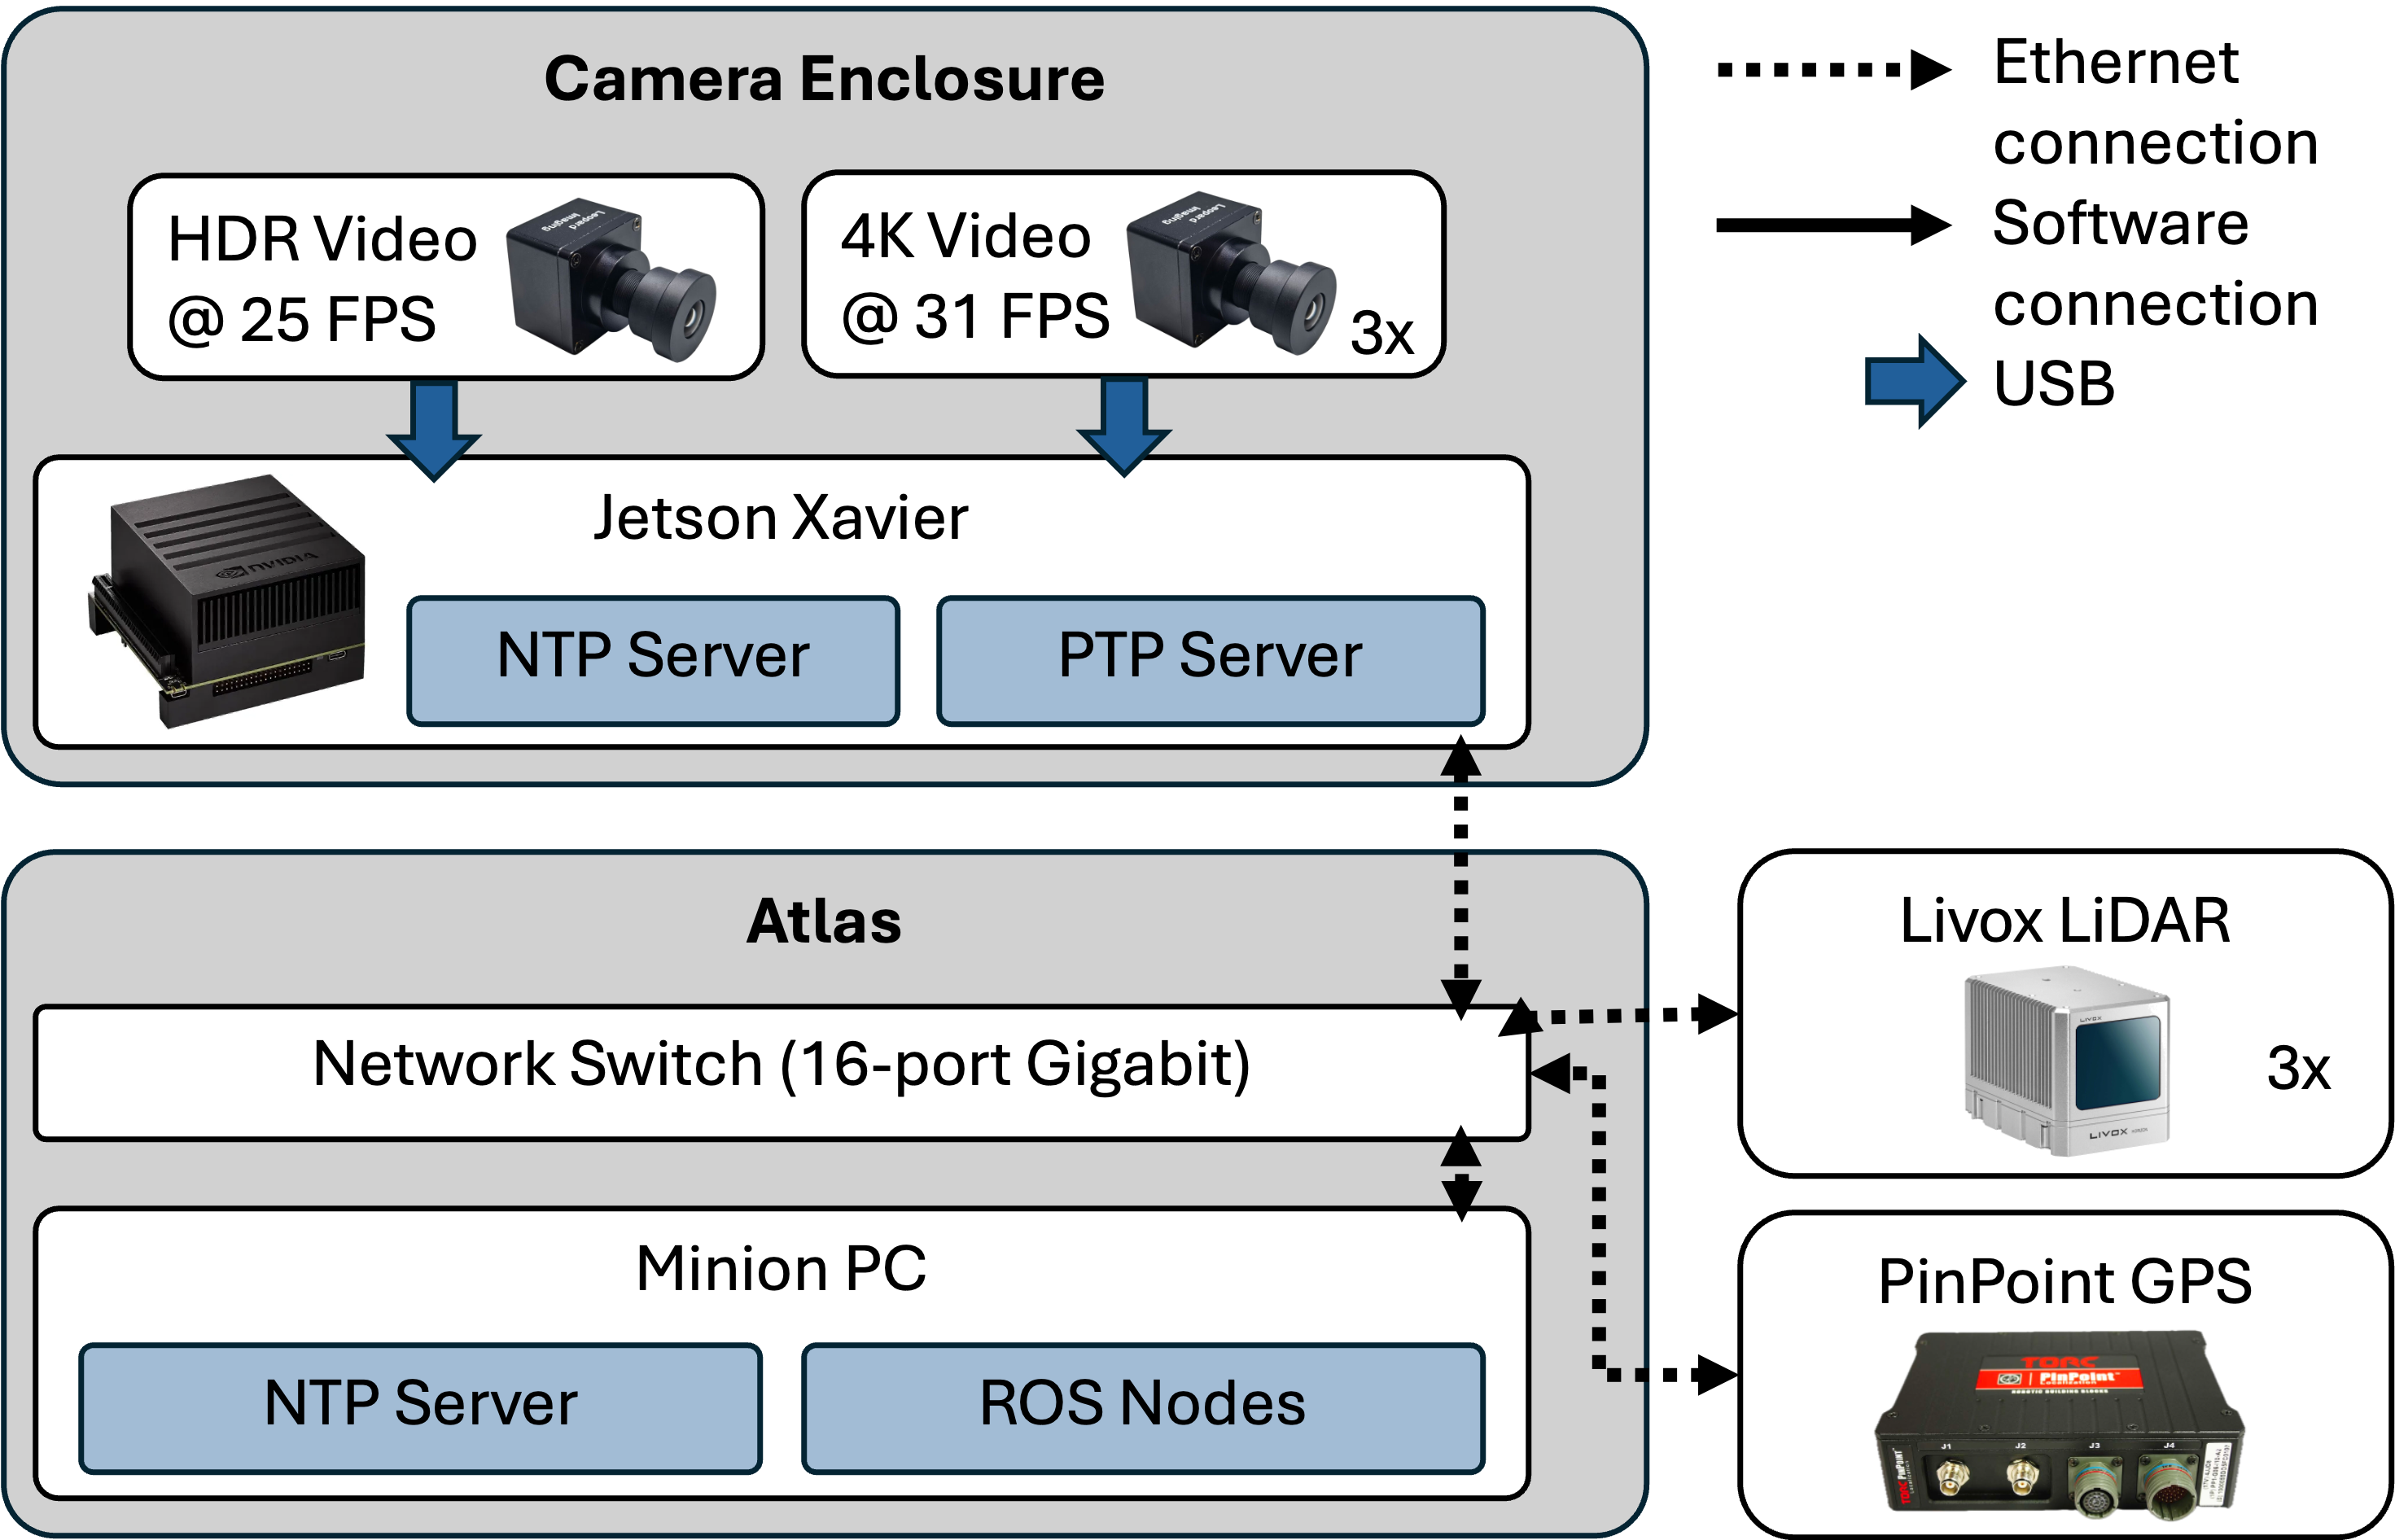
\includegraphics[width=0.8\textwidth]{Images/network_diagram2.png}
\caption{LAN diagram for Minion USV}
\label{fig:network_diagram}
\end{figure}

Although the LAN is primarily dedicated to perception and data logging, it also supports administrative access for configuration, diagnostics, and remote operation.
The Jetson Xavier is configured as a headless device and is accessed remotely via Secure Shell (SSH) for camera configuration, operation, and monitoring.
Each Minion PC can be accessed through SSH for terminal access for development tasks or troubleshooting, or Virtual Network Computing (VNC), and Remote Desktop Protocol (RDP) for a full desktop environment for system administration.
% Network security is intentionally lightweight for field deployment, relying on standard \texttt{sudo}/root authentication and a secured wireless link protected by a strong \ac{WAN} password.
Long-range connectivity between the vessel and ground station is provided by a Ubiquiti Bullet omnidirectional antenna on the \ac{USV}, paired with a directional antenna and a Ubiquiti Dream Machine at the ground station for remote system access and monitoring.

\begin{table}[htbp]
\centering
\begin{tabular}{lcc}
\hline
Data Source & Typical Bandwidth (Mbps) & \% Total Bandwidth \\
\hline
\hline
HDR Camera Stream & $3.7$--$11.2$ & $0.4$--$1.2$ \\
FLIR Camera Streams (2×) & $7.0$--$20.0$ & $0.7$--$2.1$ \\
Velodyne LiDAR Units (3x) & $43.2$--$57.6$ & $4.3$--$5.8$ \\
Livox LiDAR Units (3x) & $40.3$--$53.8$ & $4.0$--$5.4$ \\
GPS / INS Telemetry & $<0.1$ & $<0.01$ \\
Admin / SSH / Control Traffic & $0.5$--$2.0$ & $0.05$--$0.2$ \\
\hline
\textbf{Total Estimated Utilization} & \textbf{95--145 Mbps} & \textbf{9.5--14.5 \%} \\
% \hline
\end{tabular}
\caption{Approximate network bandwidth utilization from direct sensor and control data sources relative to a 1 Gbps link ($\sim940$ Mbps usable).}
\label{table:network_bandwidth}
\end{table}


\section{Sensor Calibration} \label{sec:calibration}

The multi-sensor perception suite described in the previous section integrates complementary sensing modalities: \ac{LiDAR} for spatial structure and cameras for visual context.
Each of these sensors measures the environment within its own local reference frame and according to its own internal clock.
To combine their observations into a consistent world model, the system must first be calibrated both spatially and temporally.
% Target calibration accuracy for the Minion platform was defined as less than $1^{\circ}$ rotational error, less than 1~cm translational error, and no more than 20~ms temporal offset across all sensors.

For the Minion platform, all sensors are rigidly mounted and assigned reference frames within a unified transform hierarchy. 
The GPS receiver anchors the global \texttt{map} frame; the ROS TF tree (Fig.~\ref{fig:tf_tree}) resolves transforms such as \texttt{map}\ $\rightarrow$\ \texttt{base\_link} and \texttt{base\_link}\ $\rightarrow$\ \texttt{sensor}. Spatial calibration estimates the rigid rotations and translations that populate this tree.  
Intrinsic calibration is also required for the visible-spectrum cameras (shown in blue), determining the internal optical parameters such as focal length, principal point location, and lens distortion. 
Time synchronization is similarly structured, with a master clock distributed over the network to subsystems and sensors to ensure that data acquired across sensor modalities remain temporally aligned.

% Within this framework, the port and starboard Livox units are first registered to the center Livox reference frame, where their point clouds are merged into a single unified point cloud.  
% This consolidated LiDAR frame is then related to the HDR camera world-frame through an additional extrinsic transform and finally to the camera's image-frame through the determined camera intrinsic values, allowing three-dimensional LiDAR points $(x, y, z)$ to be projected onto the two-dimensional image plane $(u, v)$ using the camera’s intrinsic parameters.  
% Finally, all perception data are kept in sync and expressed in the global map frame defined through the time, location, and orientation provided by the \ac{GPS}.
Within this framework, the port and starboard Livox units are first registered to the center Livox reference frame to produce a unified point cloud. 
The consolidated LiDAR frame is then related to the HDR camera world frame through an additional extrinsic transform. 
Using the camera’s intrinsic parameters, three-dimensional LiDAR points $(x, y, z)$ can then be projected onto the two-dimensional image plane and expressed as pixel locations $(u, v)$. 
An additional series of extrinsic transforms relates the central Livox frame to the \ac{GPS} antenna frame, and the \ac{GPS} frame to the global map frame. 
The \ac{GPS} provides dual functionality, maintaining synchronization across all sensor data and orienting them within the static global map frame.

% All perception data are synchronized and expressed in the global map frame, defined by the time, location, and orientation provided by the \ac{GPS}.

An initial calibration of the camera enclosure was performed during earlier work by Thompson~\cite{thompson2023}, establishing the baseline intrinsic camera parameters and the extrinsic relationship between the three Livox LiDAR units.
In the multiple years between data collection campaigns, the camera enclosure was relocated multiple times and subjected to extended periods of vibration during transport of the \ac{USV} on its trailer.
These mechanical stresses alone were sufficient to warrant recalibration, as small shifts in sensor mounts or camera optics can accumulate over time and degrade geometric alignment.
Compounding this, the center Livox unit suffered a hardware failure and was replaced, making a full recalibration of all extrinsic transforms essential before further data collection.

Section \ref{spatial_calibration} provides the methods used for intrinsic camera calibration, extrinsic calibration between the camera and LiDAR sensors, and between the individual LiDAR units. 
This is followed by a discussion of the time synchronization methods implemented across the network, with special detail provided to the timestamps applied to video frames in section \ref{time_sync}
Finally, the resulting spatial calibration accuracy and temporal alignment obtained are discussed in section \ref{time_sync}.



\begin{figure}[htbp]
    \centering
    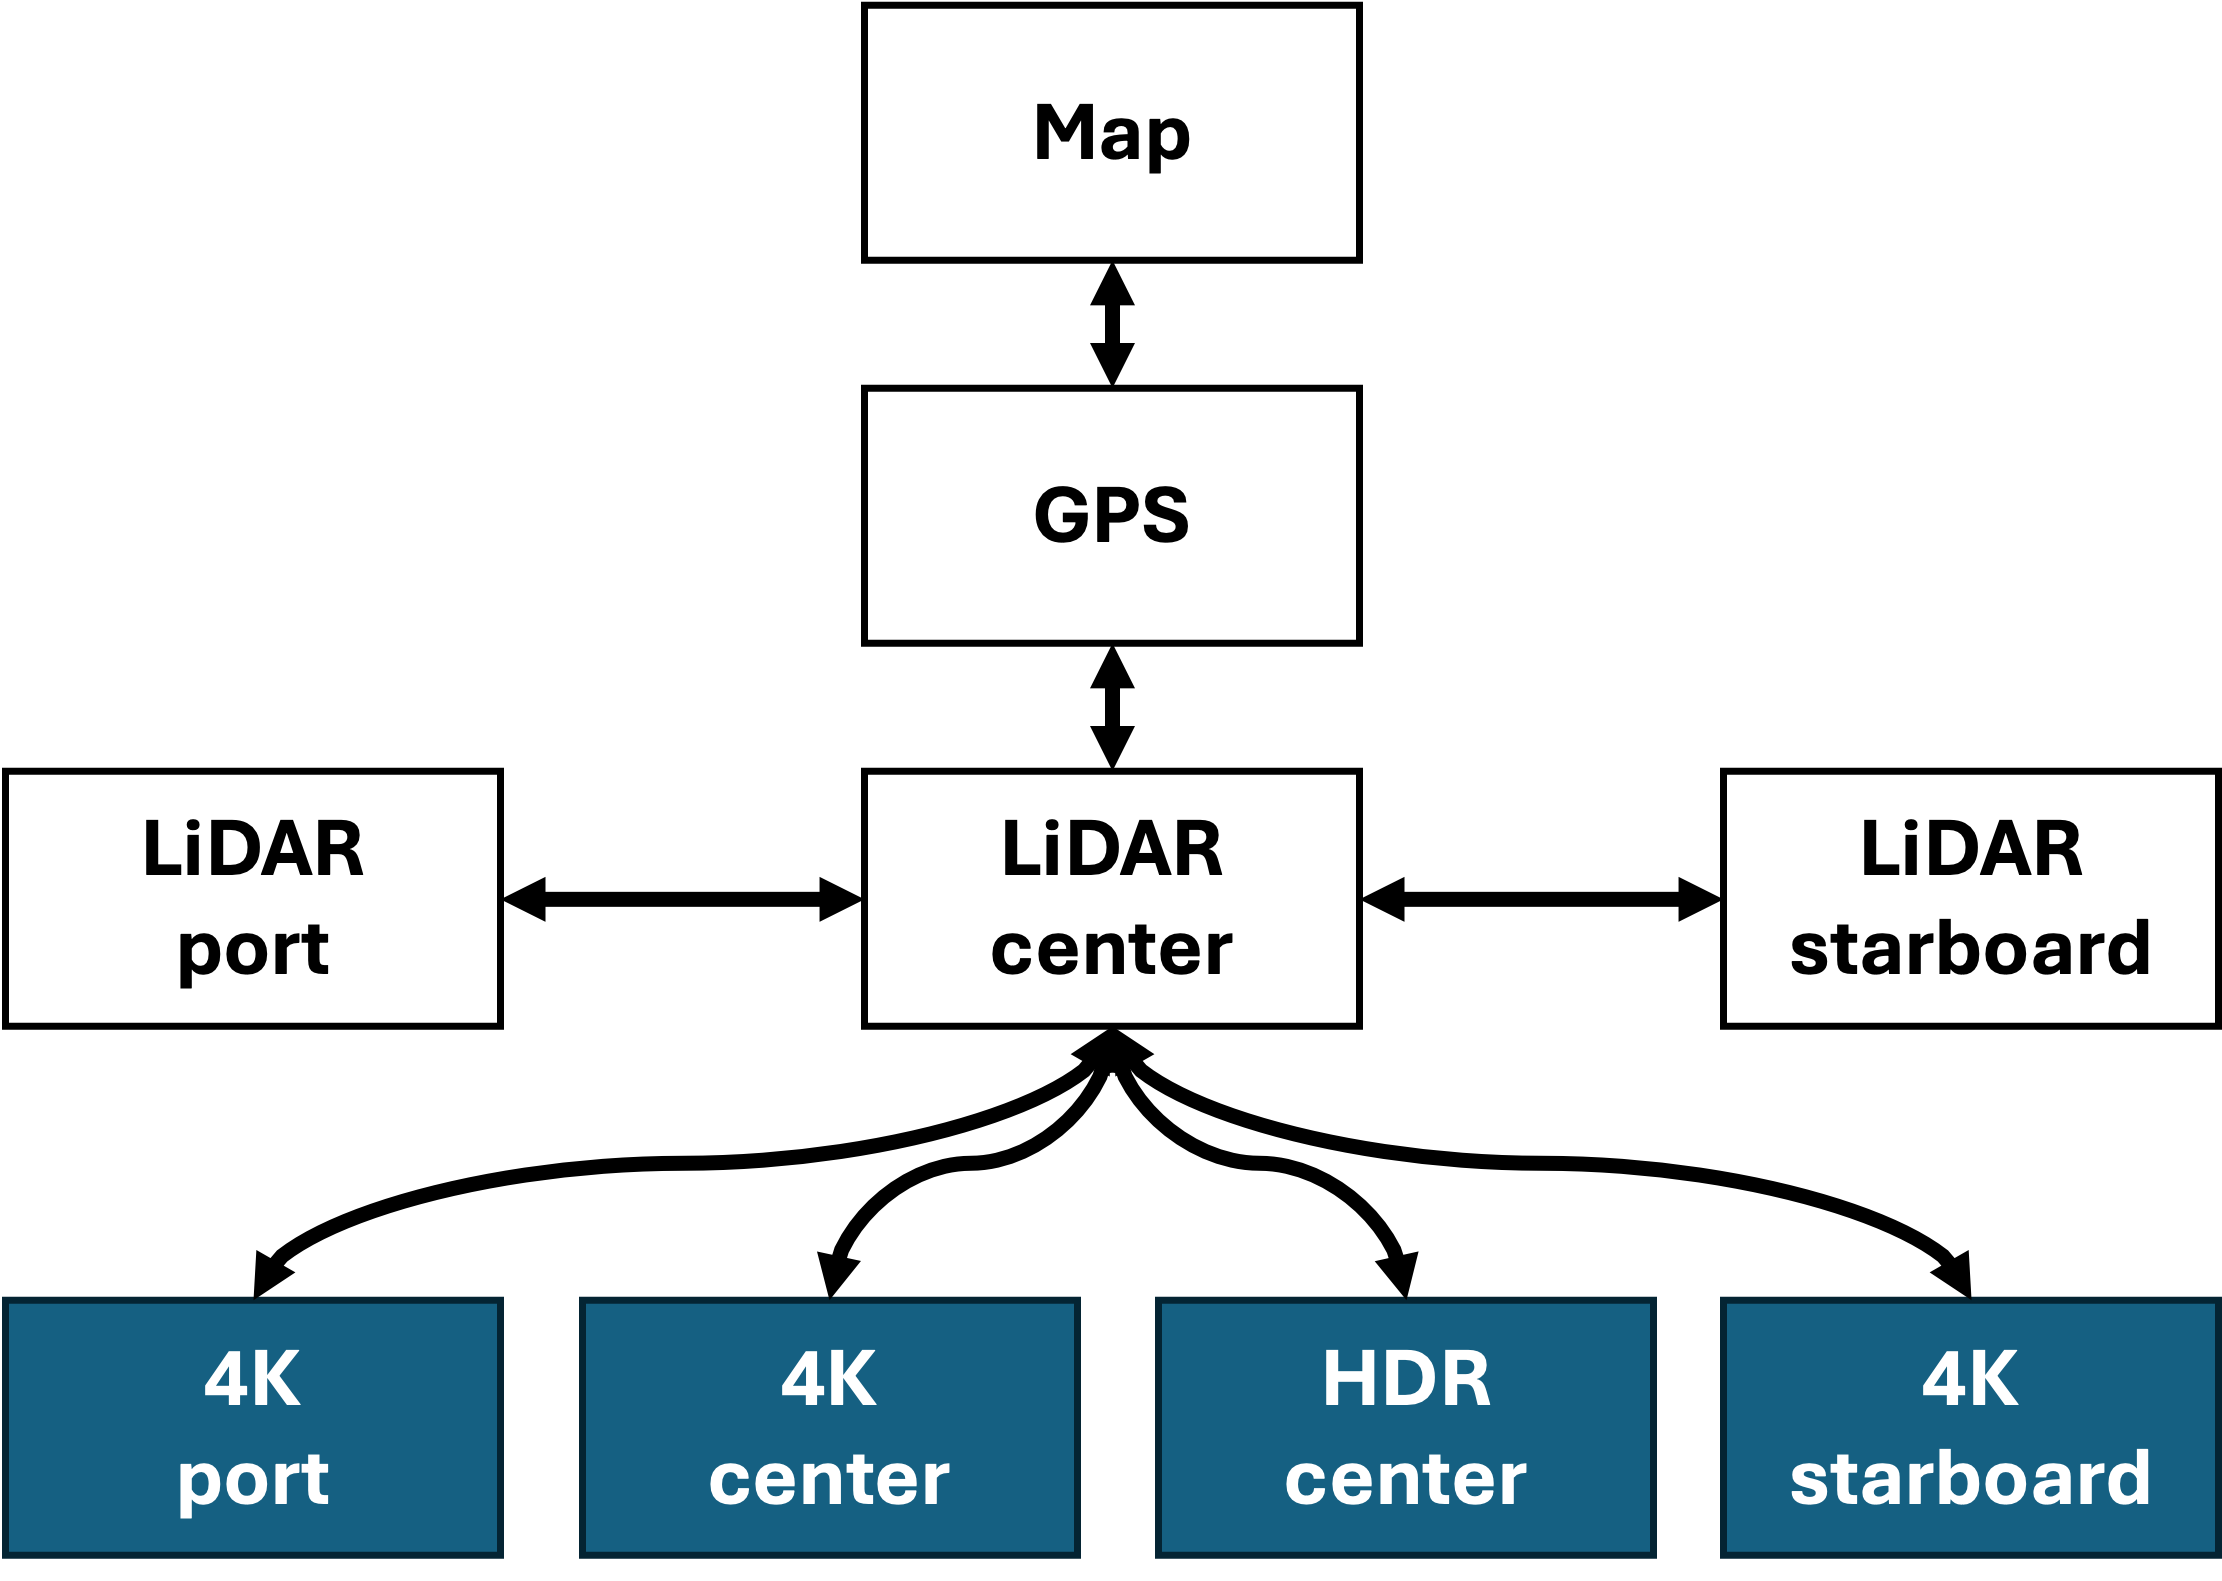
\includegraphics[width=0.7\linewidth]{Images/tf_tree_1.png}
    \caption{Transform hierarchy for Minion: the GPS-defined \texttt{map} frame anchors the ROS TF tree used for LiDAR–camera projection and sensor fusion.}
    \label{fig:tf_tree}
\end{figure}

%%%%%%%%%%%%%%%%%%%%%%%%%%%%%%%%%%%%%%%%%%%%%%%%%%%%%%%%%%%%%%%%%%%%
\subsection{Spatial Calibration} \label{spatial_calibration}

Before data from the camera and \ac{LiDAR} sensors can be combined, each device must be spatially calibrated through intrinsic and extrinsic transformations.  
This process establishes the geometric relationships required to express all sensor measurements in a unified coordinate frame, enabling accurate projection of \ac{LiDAR} points onto the camera image plane.

Calibration begins with determining the camera’s intrinsic parameters, followed by estimation of the extrinsic transformation that defines the rigid-body relationship between the camera and each \ac{LiDAR} sensor.  
The following sections describe the methods and results of this calibration process.

%%%%%%%%%%%%%%%%%%%%%%%%%%%%
\subsubsection{Extrinsic Calibration} \label{extrinsic_tform}

Extrinsic calibration defines the rigid-body transformation between two reference frames.  

The transformation from frame $A$ to frame $B$ is represented as
\begin{equation}
    _{B}^{A}\mathbf{T} =
    \begin{bmatrix}
        _{B}^{A}\mathbf{R} & _{B}^{A}\mathbf{t} \\
        \mathbf{0}^\mathrm{T} & 1
    \end{bmatrix},
\end{equation}

where $\mathbf{R}_{B}^{A} \in \mathbb{R}^{3\times3}$ is the rotation matrix describing the orientation of frame $A$ relative to frame $B$, and $_{B}^{A}\mathbf{t} \in \mathbb{R}^{3}$ is the translation vector locating the origin of frame $A$ with respect to frame $B$.  
The notation convention used here is that the subscript denotes the destination frame and the superscript the source frame.

A point $_{A}\mathbf{P}$ expressed in frame $A$ can therefore be transformed into frame $B$ as

\begin{equation}
    _{B}\mathbf{P} =
    _{B}^{A}\mathbf{R} _{A}\mathbf{P} + _{B}^{A}\mathbf{t}.
\end{equation}

This formulation provides a consistent framework for representing spatial relationships among all platform sensors.  
Transformations can be sequentially composed through the transform tree shown in Figure~\ref{fig:tf_tree}, allowing points measured by any sensor to be expressed in a common reference frame and projected into the camera image for spatial alignment.

The \ac{LiDAR}-to-\ac{LiDAR} extrinsic calibration defines the rigid-body transformations relating the three Livox Horizon units to a shared coordinate system.  
The center unit serves as the reference frame, with the port and starboard sensors calibrated relative to it to create a unified, geometrically consistent point cloud.

Using large flat surfaces such as walls or other well-defined objects within the unit's overlapping field of view allows the sensors to be aligned.
The Livox devices used have a functional detection range of 260~m \cite{livox_manual}, which is far greater than the intended operational range for the sensor fusion presented in this research. 
Due to the divergent nature of the scanning pattern, a simple visual inspection  (as illustrated in figure \ref{fig:Lidar2Lidar}) of sensor alignment beyond 100~m guarantees alignment at closer range. 

\begin{figure}[htbp]
    \centering
    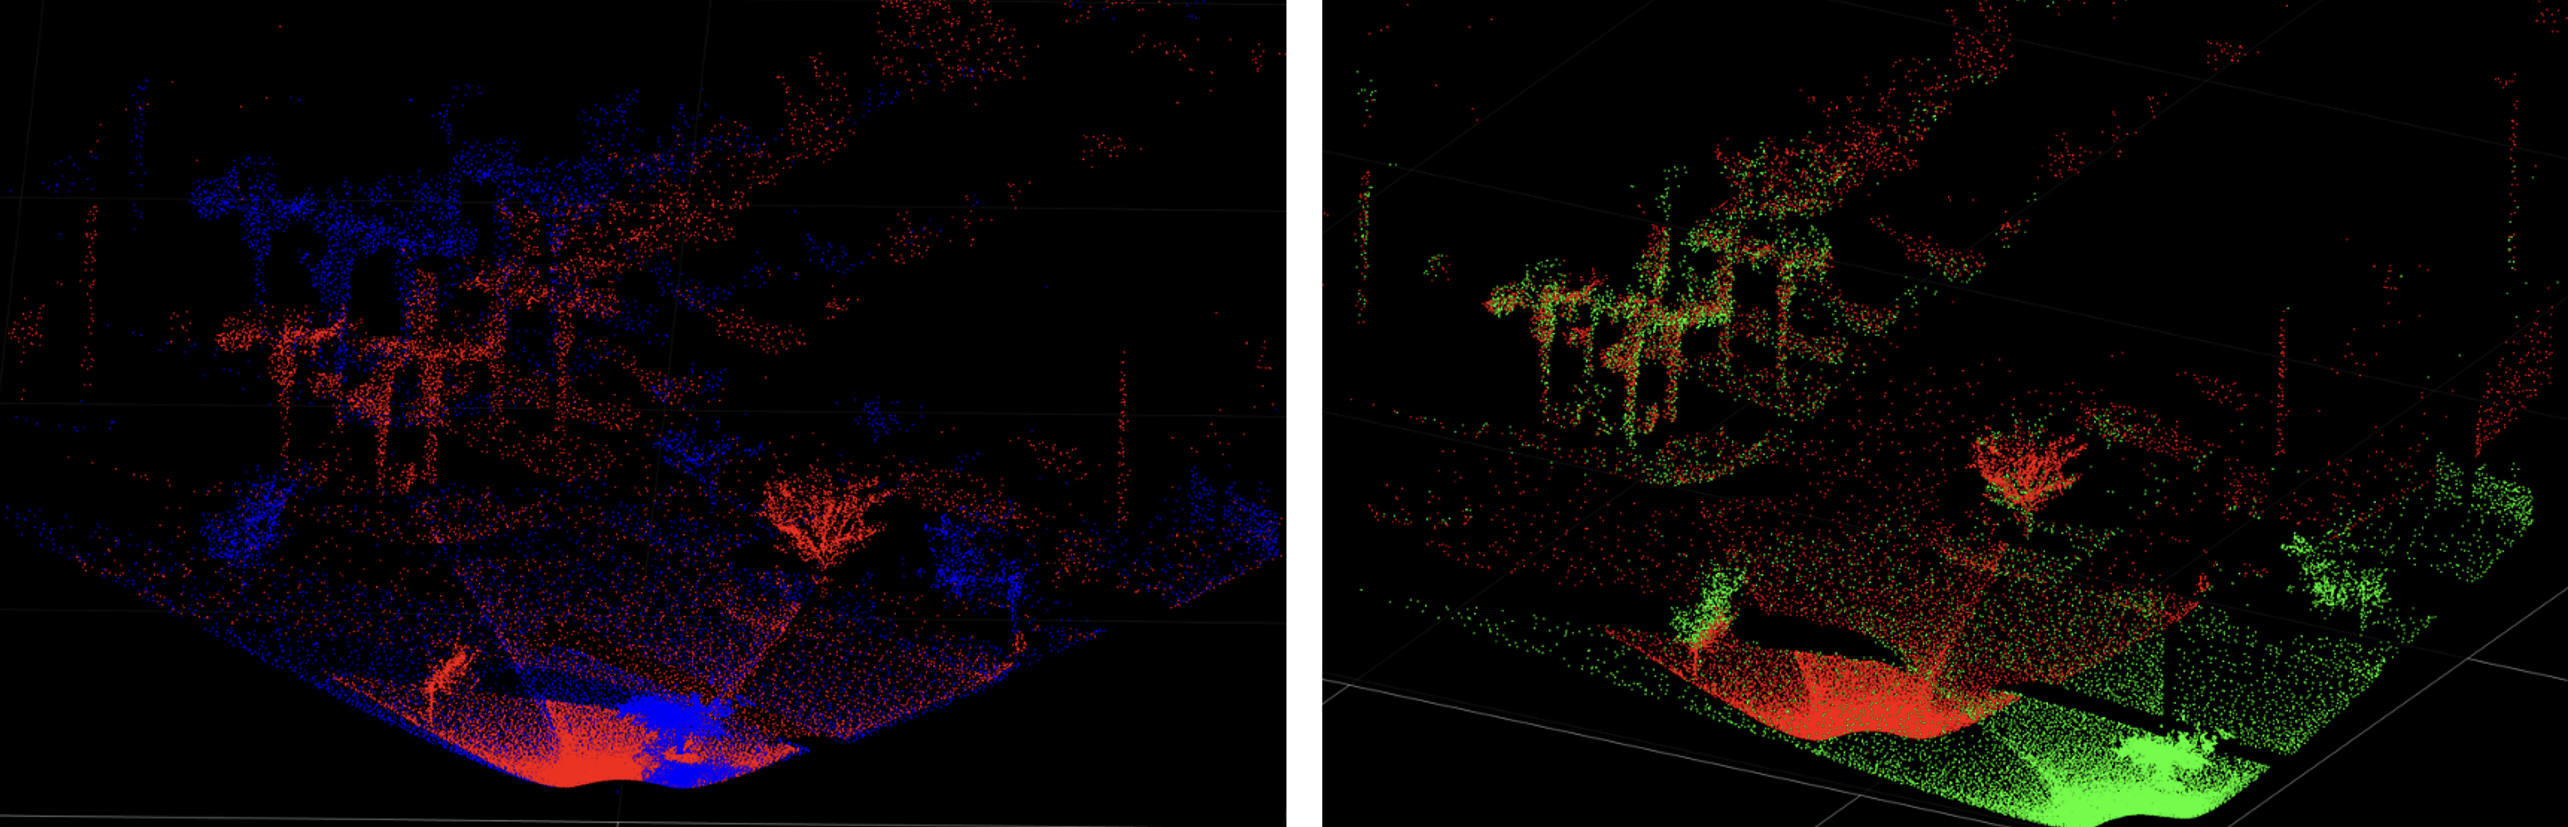
\includegraphics[width=0.9\linewidth]{Images/Lidar2Lidar.png}
    \caption{Example of LiDAR–LiDAR alignment.}
    \label{fig:Lidar2Lidar}
\end{figure}

%%%%%%%%%%%%%%%%%%%%%%%%%%%%
\subsubsection{Camera Intrinsics} \label{camera_intrinsics}

Camera intrinsic parameters describe the internal geometry of the camera and define how three-dimensional points are projected onto the two-dimensional image plane.  
They are governed by the optical pathway through the lens and determine how real-world distances correspond to image pixel coordinates.  
The intrinsic model is typically divided into an idealized pinhole projection and a lens distortion model.

Under the pinhole model, the projection of a point onto the image plane is given by the intrinsic matrix:

\begin{equation}
    \mathbf{K} = 
    \begin{bmatrix}
        f_x & s & c_x \\
        0 & f_y & c_y \\
        0 & 0 & 1
    \end{bmatrix},
\end{equation}

where $(f_x, f_y)$ are focal lengths in pixels, $(c_x, c_y)$ denotes the principal point, and $s$ represents the skew factor (generally $s=0$ for modern sensors).

Real lenses introduce distortion, primarily radial, due to refraction near the outer edge of the lens.  
This effect, most pronounced in wide-angle optics, causes straight lines to appear curved.  
Radial distortion is modeled using polynomial coefficients $k_1$, $k_2$, and $k_3$:
\begin{equation}
    \begin{split}
        x' &= x_n(1 + k_1 r^2 + k_2 r^4 + k_3 r^6), \\
        y' &= y_n(1 + k_1 r^2 + k_2 r^4 + k_3 r^6),
    \end{split}
\end{equation}

where $(x', y')$ are distorted coordinates, $(x_n, y_n)$ are ideal coordinates, and $r = \sqrt{x_n^2 + y_n^2}$ is the radial distance from the optical center.  
Although this model omits asymmetric distortions, high-quality lenses typically minimize such effects.  
Even with manufacturer-provided parameters, recalibration ensures sub-pixel accuracy when aligning \ac{LiDAR} projections with image data.

To estimate intrinsic parameters, a planar checkerboard with known square dimensions is imaged from multiple orientations and distances.  
Its grid of high-contrast corners serves as stable reference points for gradient-based corner detection algorithms such as the Harris method.  
Calibration software uses these detected points to compute statistically optimal parameters across the full image set.

Effective calibration requires dozens of images taken at diverse depths and orientations spanning the camera’s operational field of view.  
Checkerboard dimensions should approximate the scale of observed objects to ensure that the chosen camera provides adequate spatial resolution (as discussed in Section~\ref{camera_selection}).  
Following these practices produces robust intrinsic estimates across the full imaging range.

\begin{figure}[htbp]
\centering
\makebox[\textwidth][c]{%
    \begin{subfigure}[t]{0.3\textwidth}
        \centering
        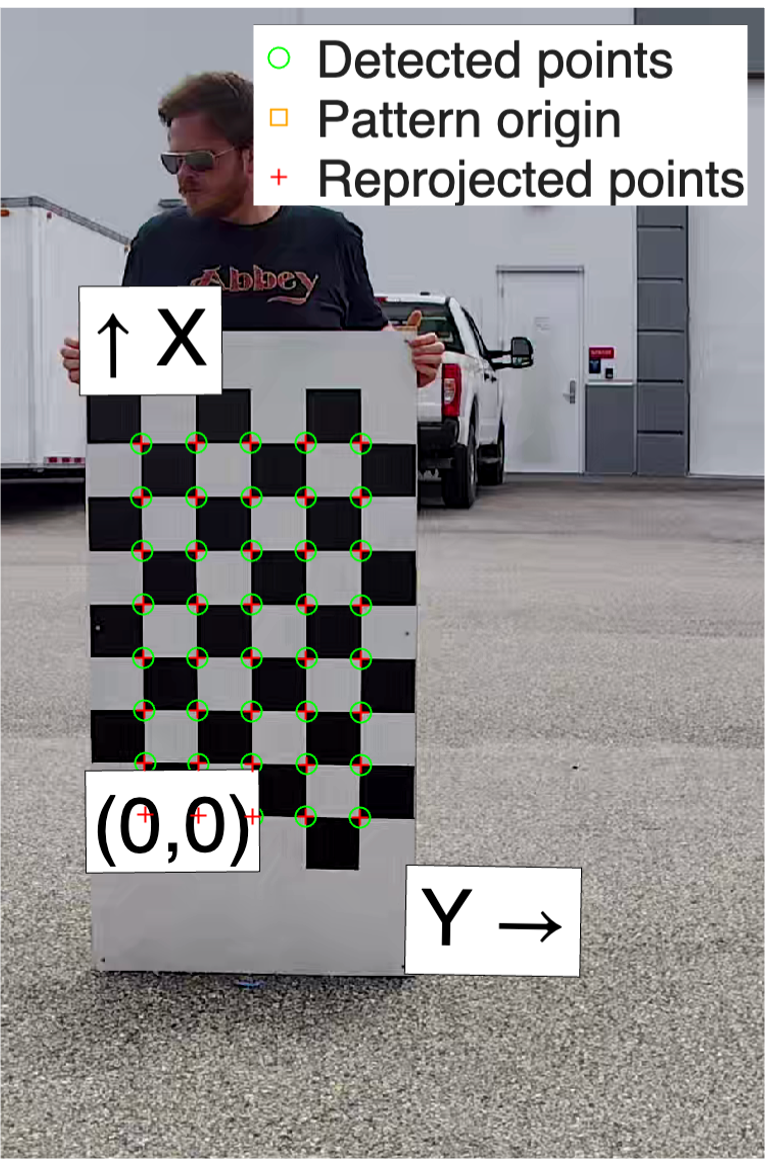
\includegraphics[width=\textwidth]{Images/cam_calib_1.png}
        \caption{A single example of detected and reprojected checkerboard corners. Agreement between detected (green circles) and reprojected (red crosses) points demonstrates corner localization and mapping of the image coordinate system.}
        \label{fig:cam_calib_1}
    \end{subfigure}
    \hspace{2em}
    \begin{subfigure}[t]{0.625\textwidth}
        \centering
        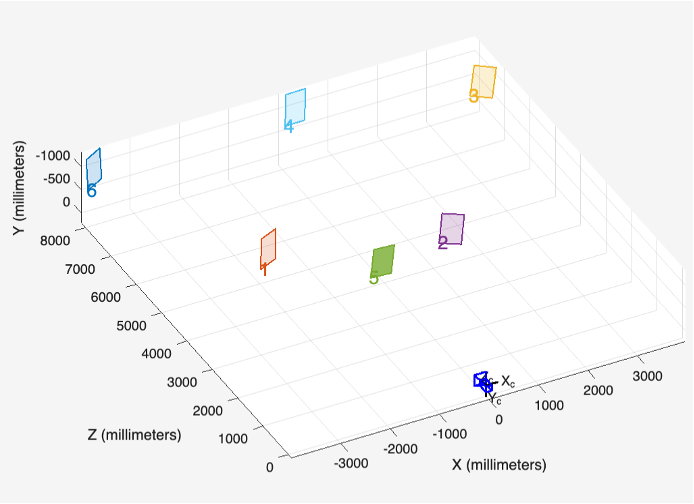
\includegraphics[width=\textwidth]{Images/cam_calib_2.png}
        \caption{Reprojection of sample target poses into the 3D world frame after calibration.}
        \label{fig:cam_calib_2}
    \end{subfigure}%
}
\caption{Checkerboard images are processed to detect corners (left), which enable intrinsic parameters to be estimated and validated by reprojecting known targets into 3D space (right).}
\label{fig:cam_calib}
\end{figure}


%%%%%%%%%%%%%%%%%%%%%%%%%%%%
\subsubsection{Camera to LiDAR Extrinsic Calibration} \label{camLidar_calib}

Camera–LiDAR calibration begins by positioning a planar checkerboard target within both the LiDAR field of view and the camera image.  
The target’s physical dimensions in the LiDAR frame $(X_L, Y_L, Z_L)$ are matched to corresponding pixel coordinates $(u,v)$ in the image, yielding an initial estimate of the rigid transformation between sensor frames.  
A full derivation of this mapping is given in Appendix~\ref{img_tform}, and an example is shown in Figure~\ref{fig:calib_check}.

Initial calibration is performed using software such as the MATLAB LiDAR Calibration tool \cite{matlab_calibration}.  
Further refinement can be achieved either through iterative manual adjustment or by applying an \ac{ICP} algorithm, which minimizes point-to-plane error between the LiDAR point cloud and the camera-projected checkerboard corners.  
This approach produces a coarse transformation $_{C}^{L}\mathbf{T}$ adequate for accurate projection of LiDAR points into the image frame.

Manual fine-tuning may then be conducted by aligning prominent environmental features—such as walls, trees, and fences—visible in both modalities.  
This visual refinement yields sub-degree rotational and centimeter-level translational precision, sufficient for high-accuracy sensor fusion and object-detection tasks.  
In some cases, minor adjustments to the camera intrinsics are also necessary to compensate for small propagated errors.

\begin{figure}[htbp]
\centering
\makebox[\textwidth][c]{
    \begin{subfigure}[t]{0.44\textwidth}
        \centering
        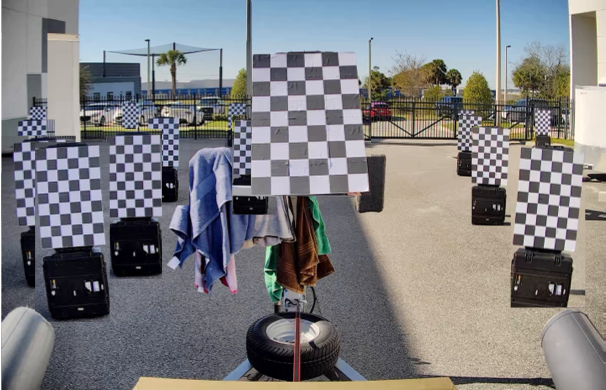
\includegraphics[width=\textwidth]{Images/checkerboard.png}
        \caption{Composite image of multiple checkerboard target locations.}
        \label{fig:checkerboard}
    \end{subfigure}
    \hspace{2em}
    \begin{subfigure}[t]{0.44\textwidth}
        \centering
        \includegraphics[width=\textwidth]{Images/LiDAR_calib.png}
        \caption{Composite of checkerboard locations in the LiDAR reference frame.}
        \label{fig:LiDAR_calib}
    \end{subfigure}
}
\caption{Checkerboard targets used for camera intrinsic (left) and LiDAR extrinsic (right) calibration. Red dots mark detected corner points transformed into the LiDAR frame using the initial extrinsic estimate.}
\label{fig:camLidar_calib}
\end{figure}


%%%%%%%%%%%%%%%%%%%%%%%%%%%%%%%%%%%%%%%%%%%%%%%%%%%%%%%%%%%%%%%%%%%%
\subsection{Results: Spatial Calibration}
\label{sec:spatial_calib_results}
%%%%%%%%%%%%%%%%%%%%%%%%%%%%
\subsubsection{LiDAR–LiDAR Calibration} \label{results_lidarLidar_calib}

% Calibration was performed using the manufacturer’s Livox Viewer software, which provides real-time point cloud visualization and the ability to view, modify, and store sensor extrinsic measurements on-device.
% This interface enables manual adjustment and fine-tuning to minimize misalignment across large planar surfaces such as walls.  
% Once optimal alignment is achieved, the extrinsic parameters can be stored in each sensor’s onboard memory.
% The port and starboard Livox units use this information to transform the data into the central Livox frame prior to transmission, reducing the computational load on Atlas. 

Calibration was performed using the Livox Viewer software, which provides real-time multi-sensor point cloud visualization and tools for automatic calibration and manual adjustment of extrinsic parameters (as shown in Figure~\ref{fig:LidarLidar_calib}). 
The calibration process involved fine-tuning of the $x, y, z$ distance and roll, pitch, and yaw between sensors.
% until a consistent alignment was achieved across overlapping fields of view, using the large planar surfaces of the laboratory walls as a reference. 
Calibration accuracy was then verified through visual inspection of large, well-defined environmental features such as trees and buildings at distances of 100–200~m, confirming consistent alignment across all three sensors.
Once satisfactory alignment was reached, the resulting parameters were recorded and written to the respective sensor’s onboard memory, where the transformation can be applied before data transmission, thus minimizing downstream computation. 

\begin{figure}[ht]
\centering
        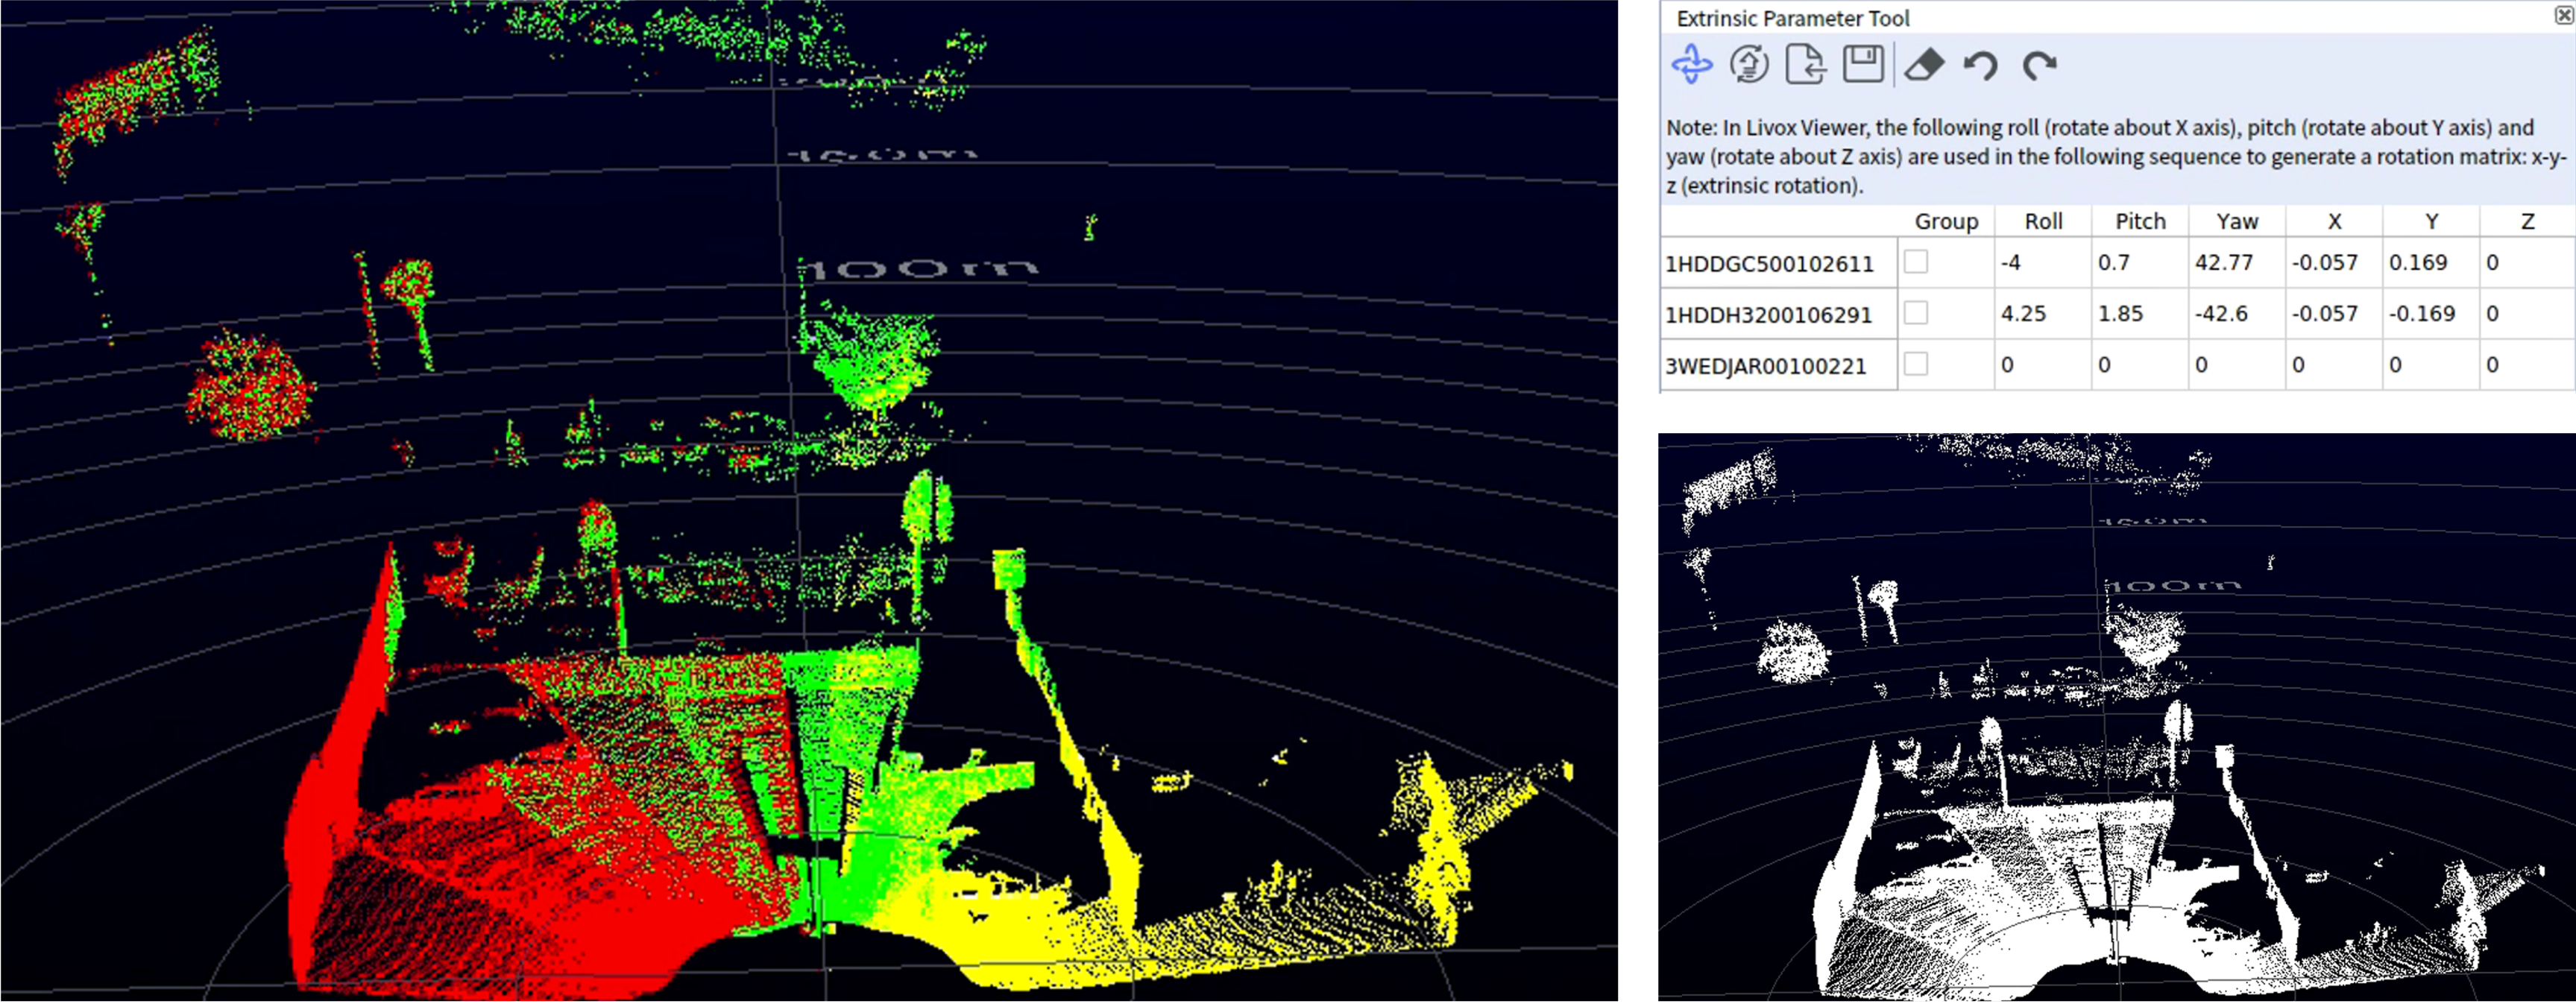
\includegraphics[width=0.95\textwidth]{Images/livox_viewer.png} 
\caption{Data from port (red), center (green), and starboard (yellow) Livox Units as viewed within the Livox Viewer software (left), and the integrated calibration tool with estimated extrinsic parameters shown (right). }
\label{fig:LidarLidar_calib}
\end{figure}

% \textcolor{red}{Insert Image from Livox Viewer Showing alignment}
%%%%%%%%%%%%%%%%%%%%%%%%%%%%
\subsubsection{Camera Calibration} \label{sec:camera_intriniscs_results}

Camera calibration was performed using a newly fabricated checkerboard target, shown in Figures~\ref{fig:checkerboard_old} and~\ref{fig:checkerboard_new}.  
The target consists of a 6$\times$9 grid of 100~mm squares, providing 40 corner features for registration.  
Thirty HDR images were captured with the checkerboard placed at positions spanning the horizontal field of view and distances between five and 40~m.
These images were then processed with MATLAB Camera Calibration app \cite{matlab_calibration}, which was successful in detecting the checkerboard in 23 separate frames.  
This initial process provided a set of camera intrinsic values with a mean pixel error of 0.63~pixels (Figure~\ref{fig:HDR_calib_error}).

\begin{figure}[htbp]
    \centering
    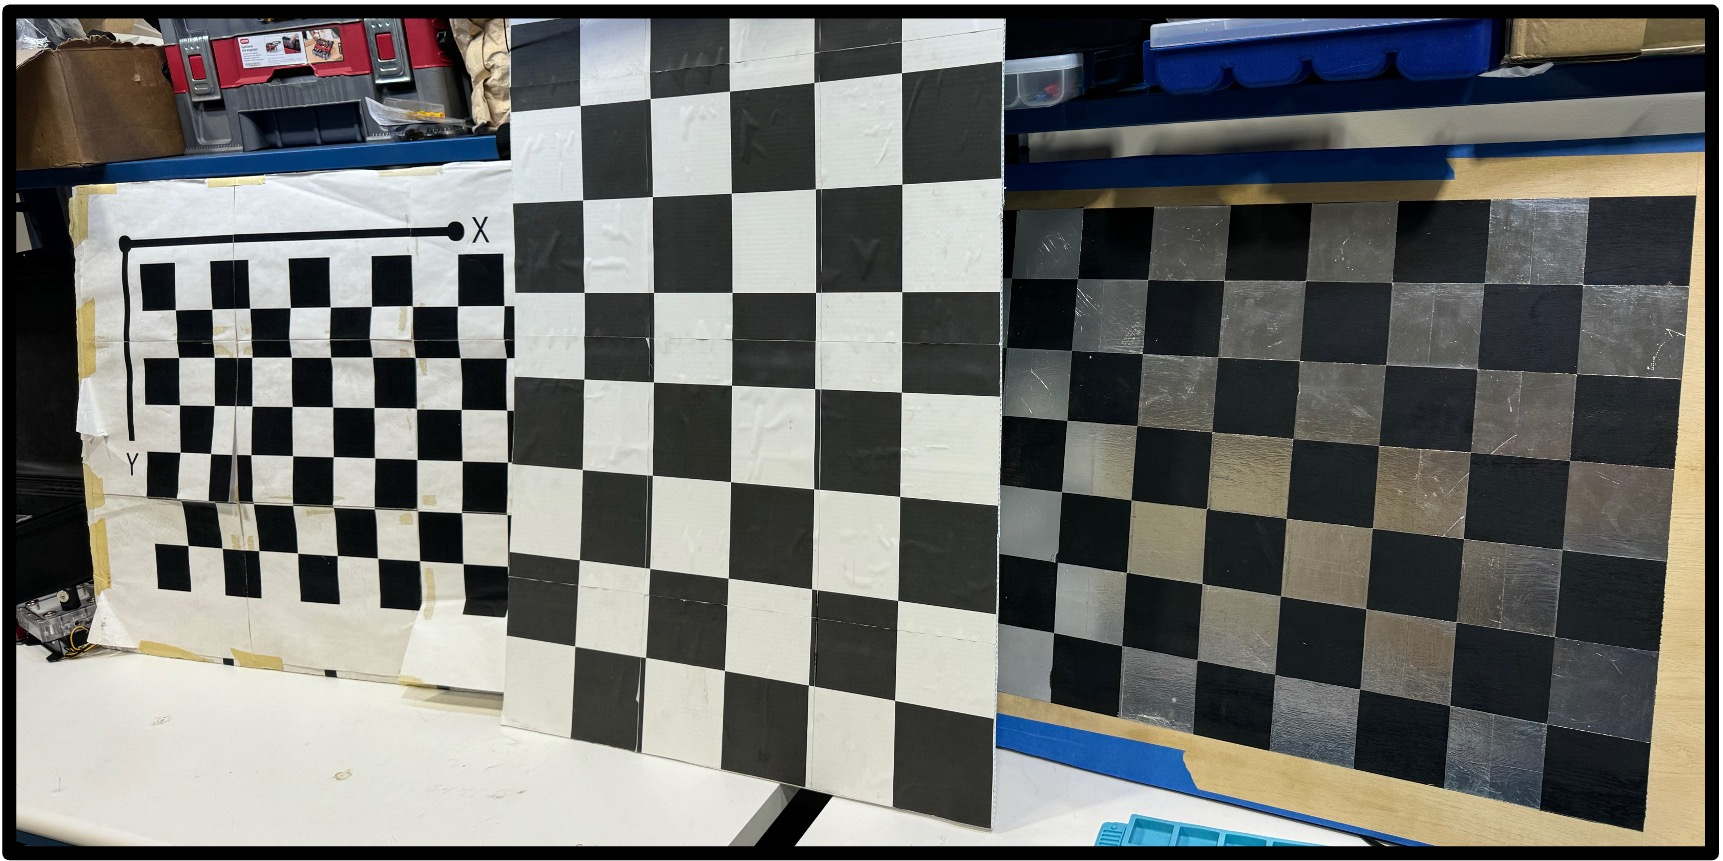
\includegraphics[width=0.9\linewidth]{Images/checkerboard_old.jpg}
    \caption{Older paper-based checkerboards maintained dimensional accuracy but degraded over time.}
    \label{fig:checkerboard_old}
\end{figure}

\begin{figure}[htbp]
    \centering
    \includegraphics[width=0.9\linewidth]{Images/Checkerboard_new.png}
    \caption{New precision-painted checkerboard target used for intrinsic calibration.}
    \label{fig:checkerboard_new}
\end{figure}

\begin{figure}[htbp]
    \centering
    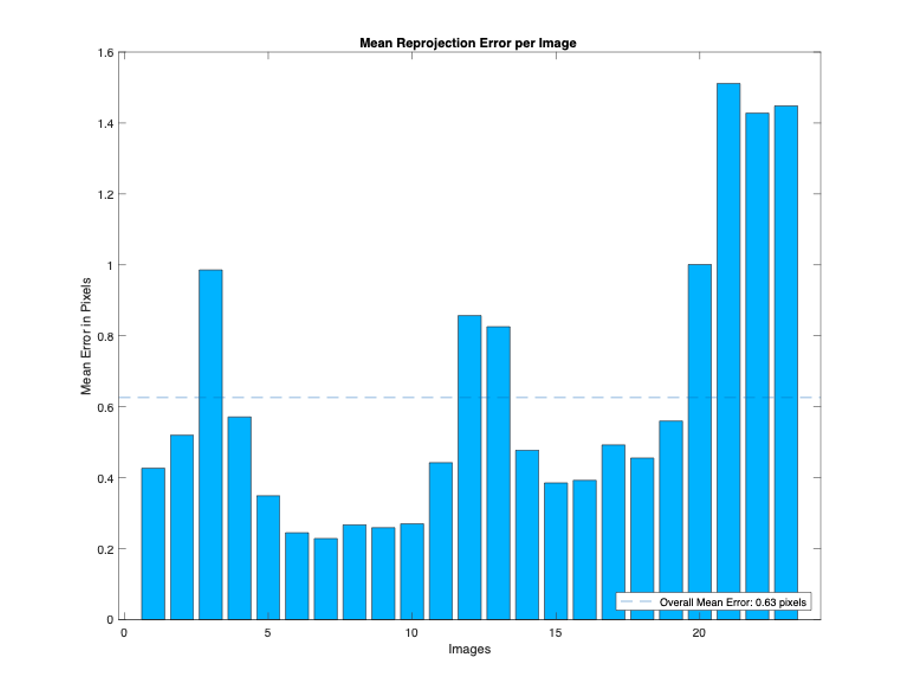
\includegraphics[width=0.9\linewidth]{Images/HDR_calib_error.png}
    \caption{Initial HDR camera calibration yielded a mean re-projection error of 0.63~pixels across the dataset.\textcolor{red}{reproduce graphic with larger text and landscape orientation. no need for square aspect ratio.}}
    \label{fig:HDR_calib_error}
\end{figure}

% The resulting transformation achieved sub-degree rotational and centimeter-level translational accuracy, sufficient for reliable fusion and object detection.
%%%%%%%%%%%%%%%%%%%%%%%%%%%%
\subsubsection{Camera–LiDAR Calibration} \label{sec:camera-lidar_results}

During extrinsic calibration, the same checkerboard images were concurrently scanned by the LiDAR.  
Each frame was held stationary while the LiDAR accumulated data over 0.5 seconds, producing a dense point cloud of the target even at ranges up to 12~m.  
These data were segmented into \acp{ROI}, matched to their corresponding image frames, and processed within MATLAB’s LiDAR Calibration tool \cite{matlab_calibration} to derive the initial extrinsic transformation.

\begin{figure}[htbp]
    \centering
    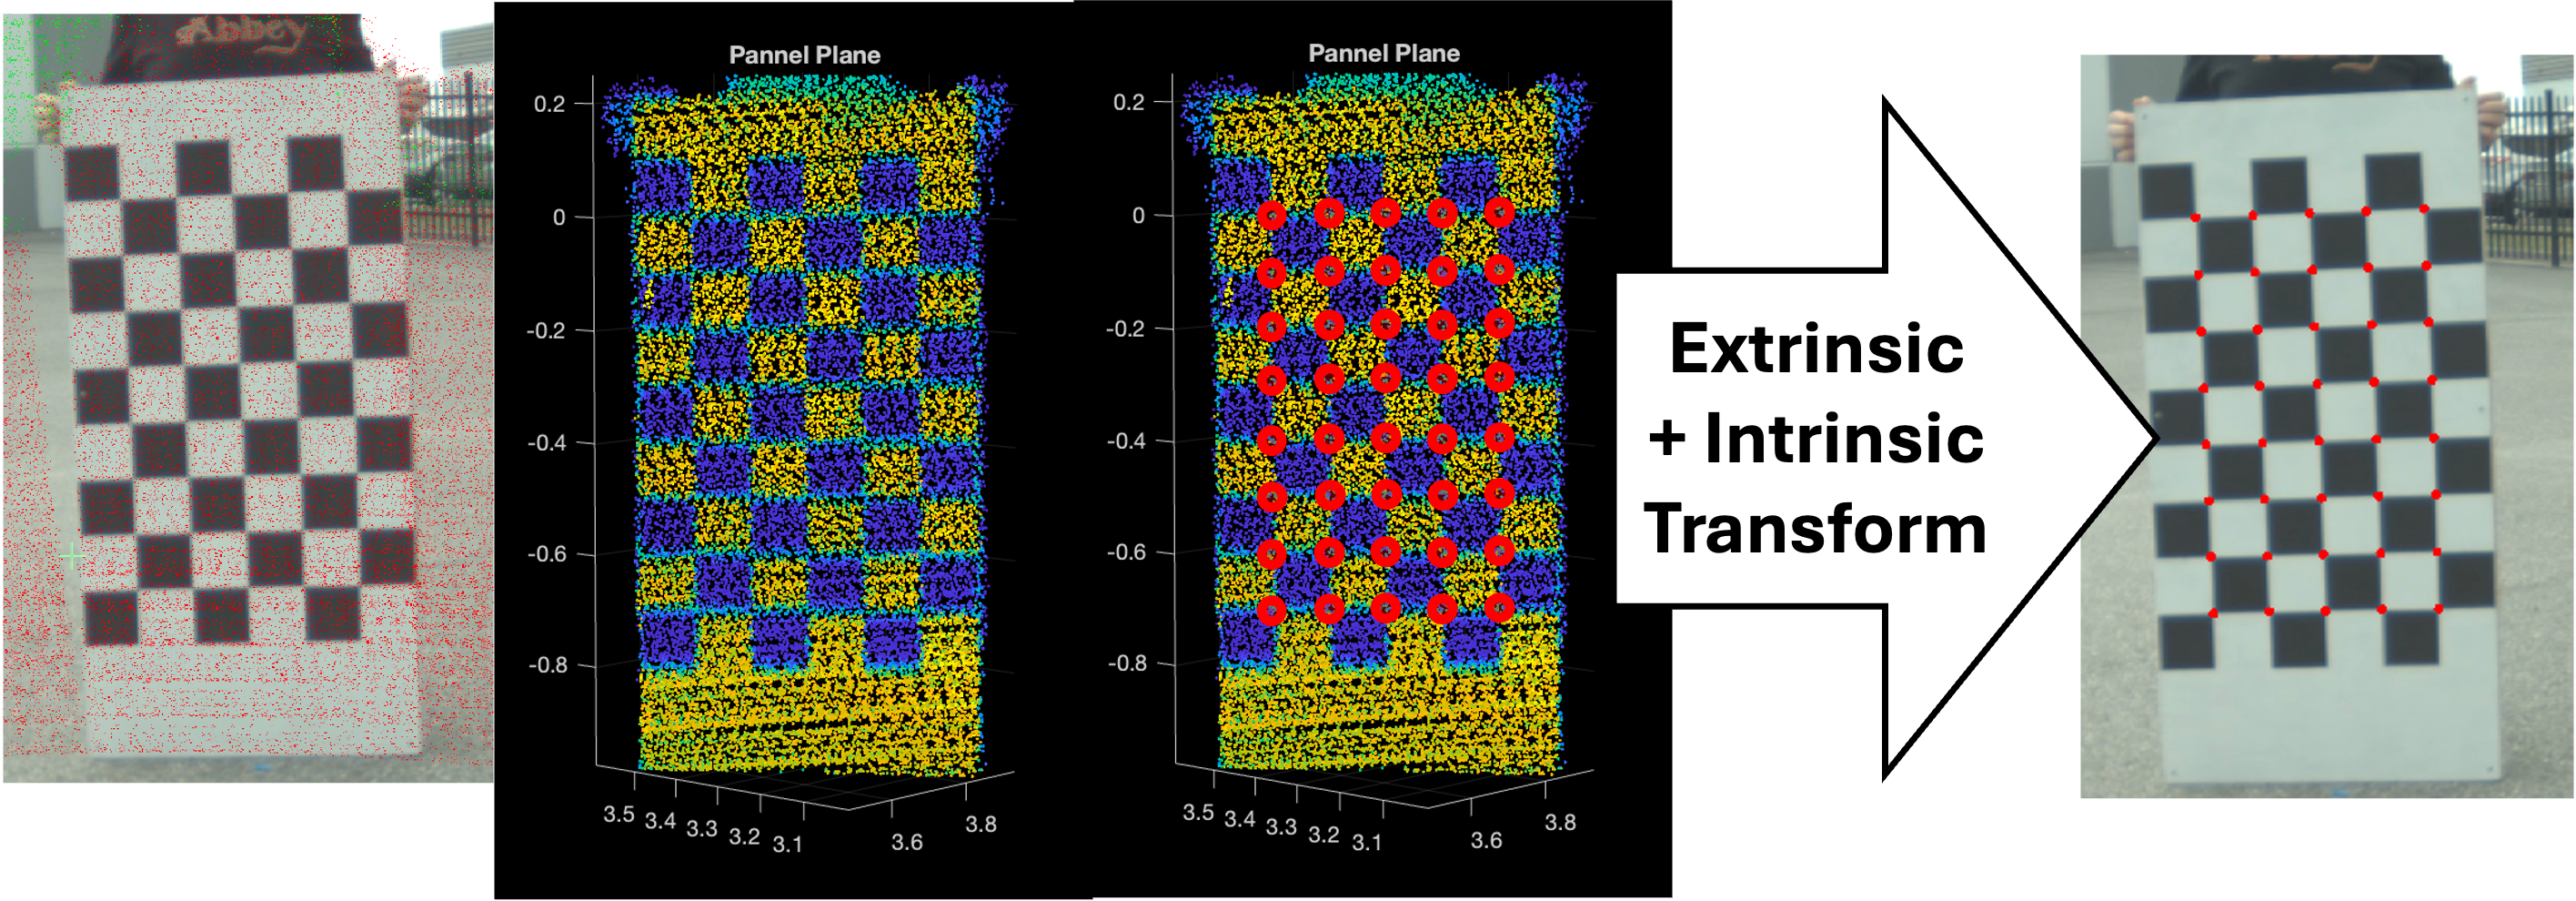
\includegraphics[width=0.8\linewidth]{Images/calib_checkers.png}
    \caption{Example of matched LiDAR point cloud and camera checkerboard detections used for extrinsic calibration.}
    \label{fig:calib_check}
\end{figure}

Subsequent manual refinement was conducted by aligning environmental features visible in both modalities, such as fences, walls, and trees, as shown in Figure~\ref{fig:LiDAR_overlay3A}.  
This process improved both extrinsic and intrinsic parameter consistency and yielded substantially higher projection fidelity.  
Comparison between early and final calibration results can be seen by comparing Figures~\ref{fig:LiDAR_overlay4} and~\ref{HDR_calib_final}.

\begin{figure}[htp]
\begin{subfigure}{\textwidth}
\centering
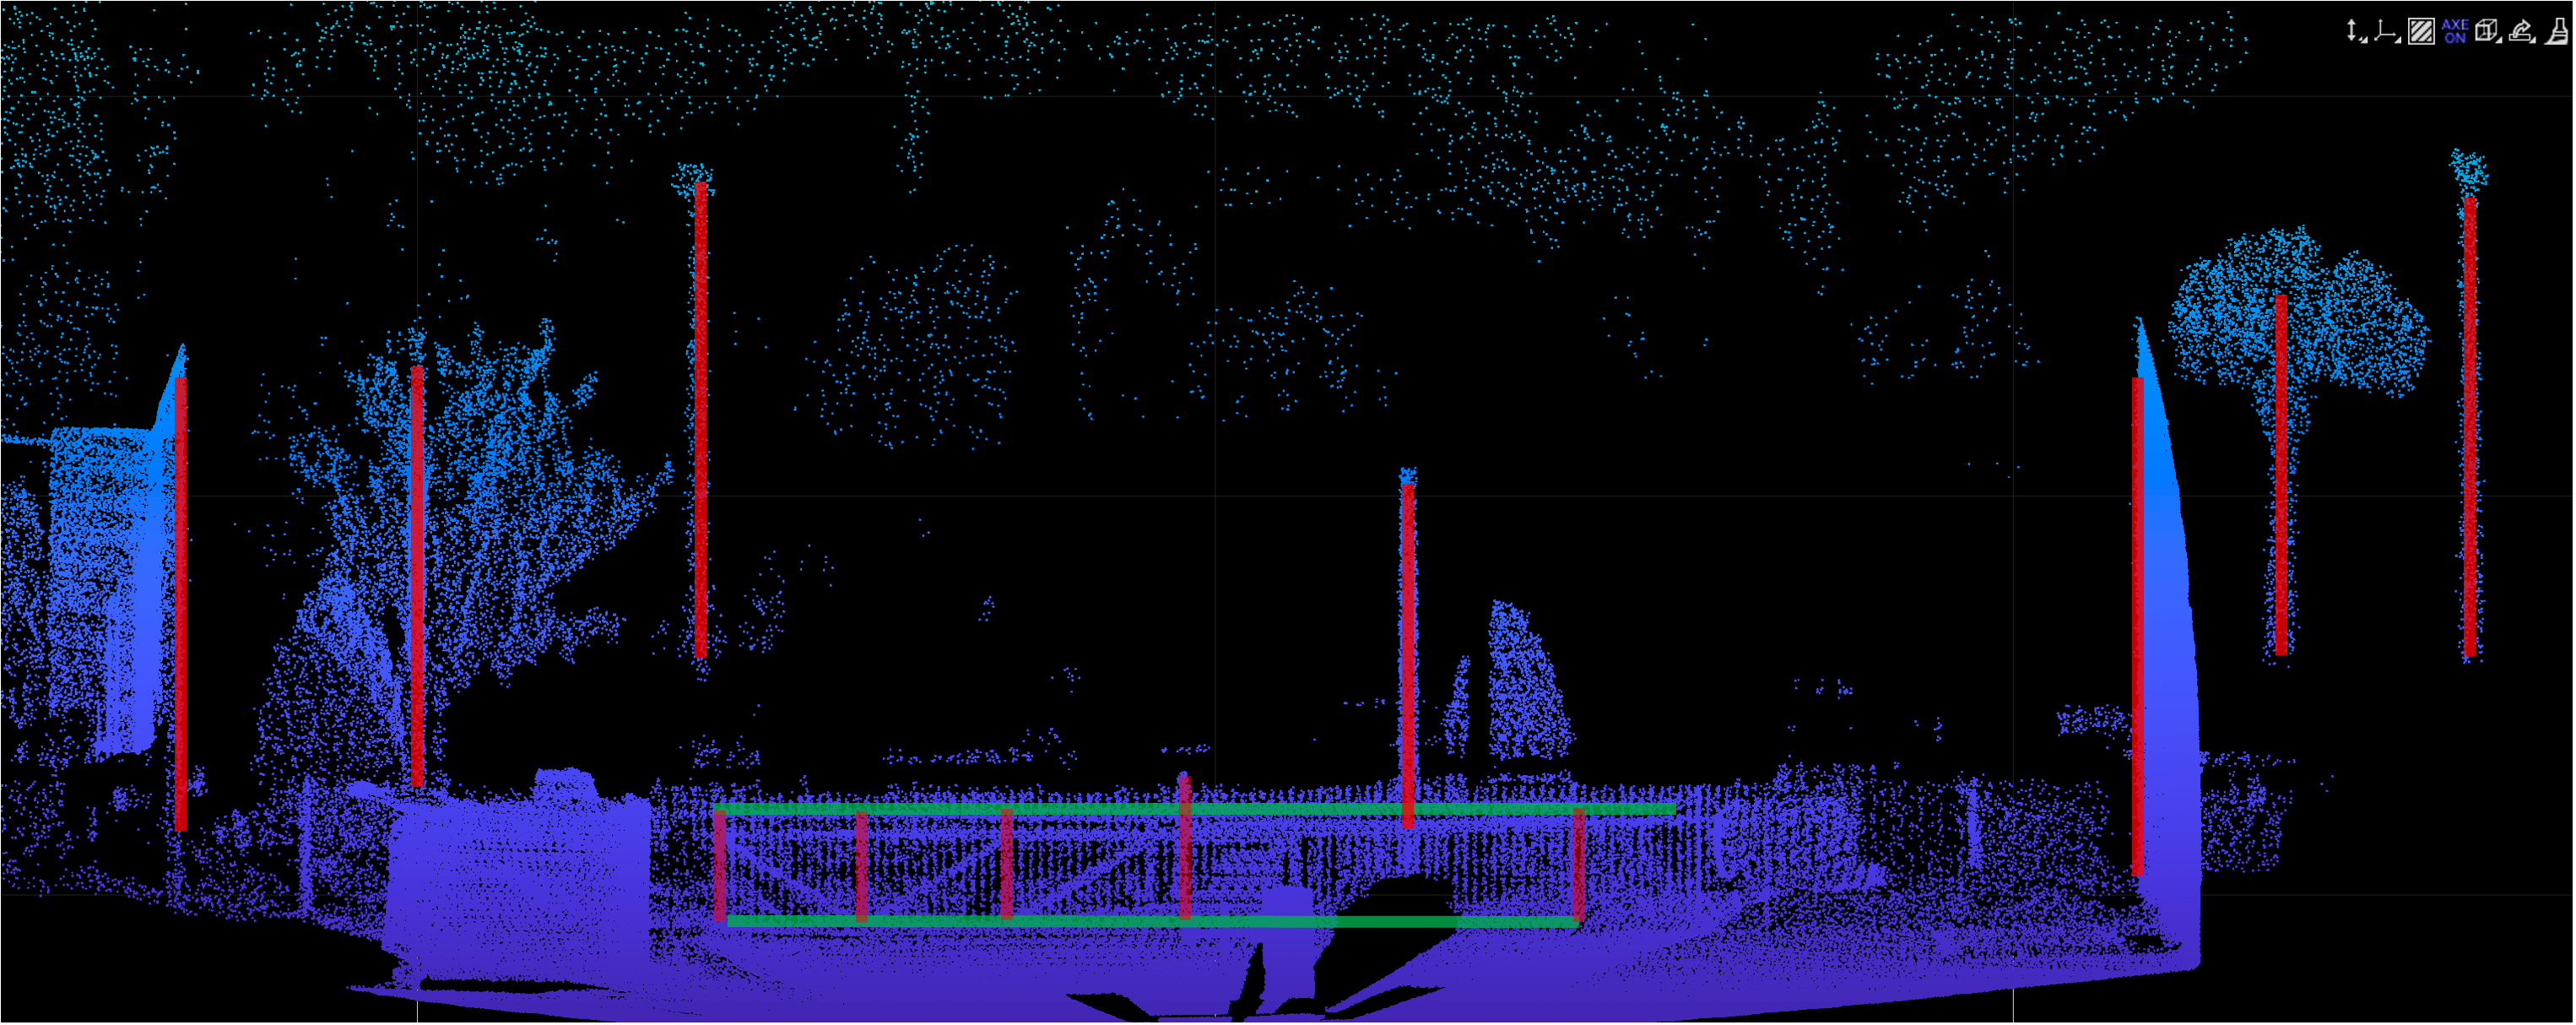
\includegraphics[width=0.94\linewidth]{Images/LiDAR_features.png}
    \caption{}
\end{subfigure}
\bigskip
\begin{subfigure}{\textwidth}
\centering
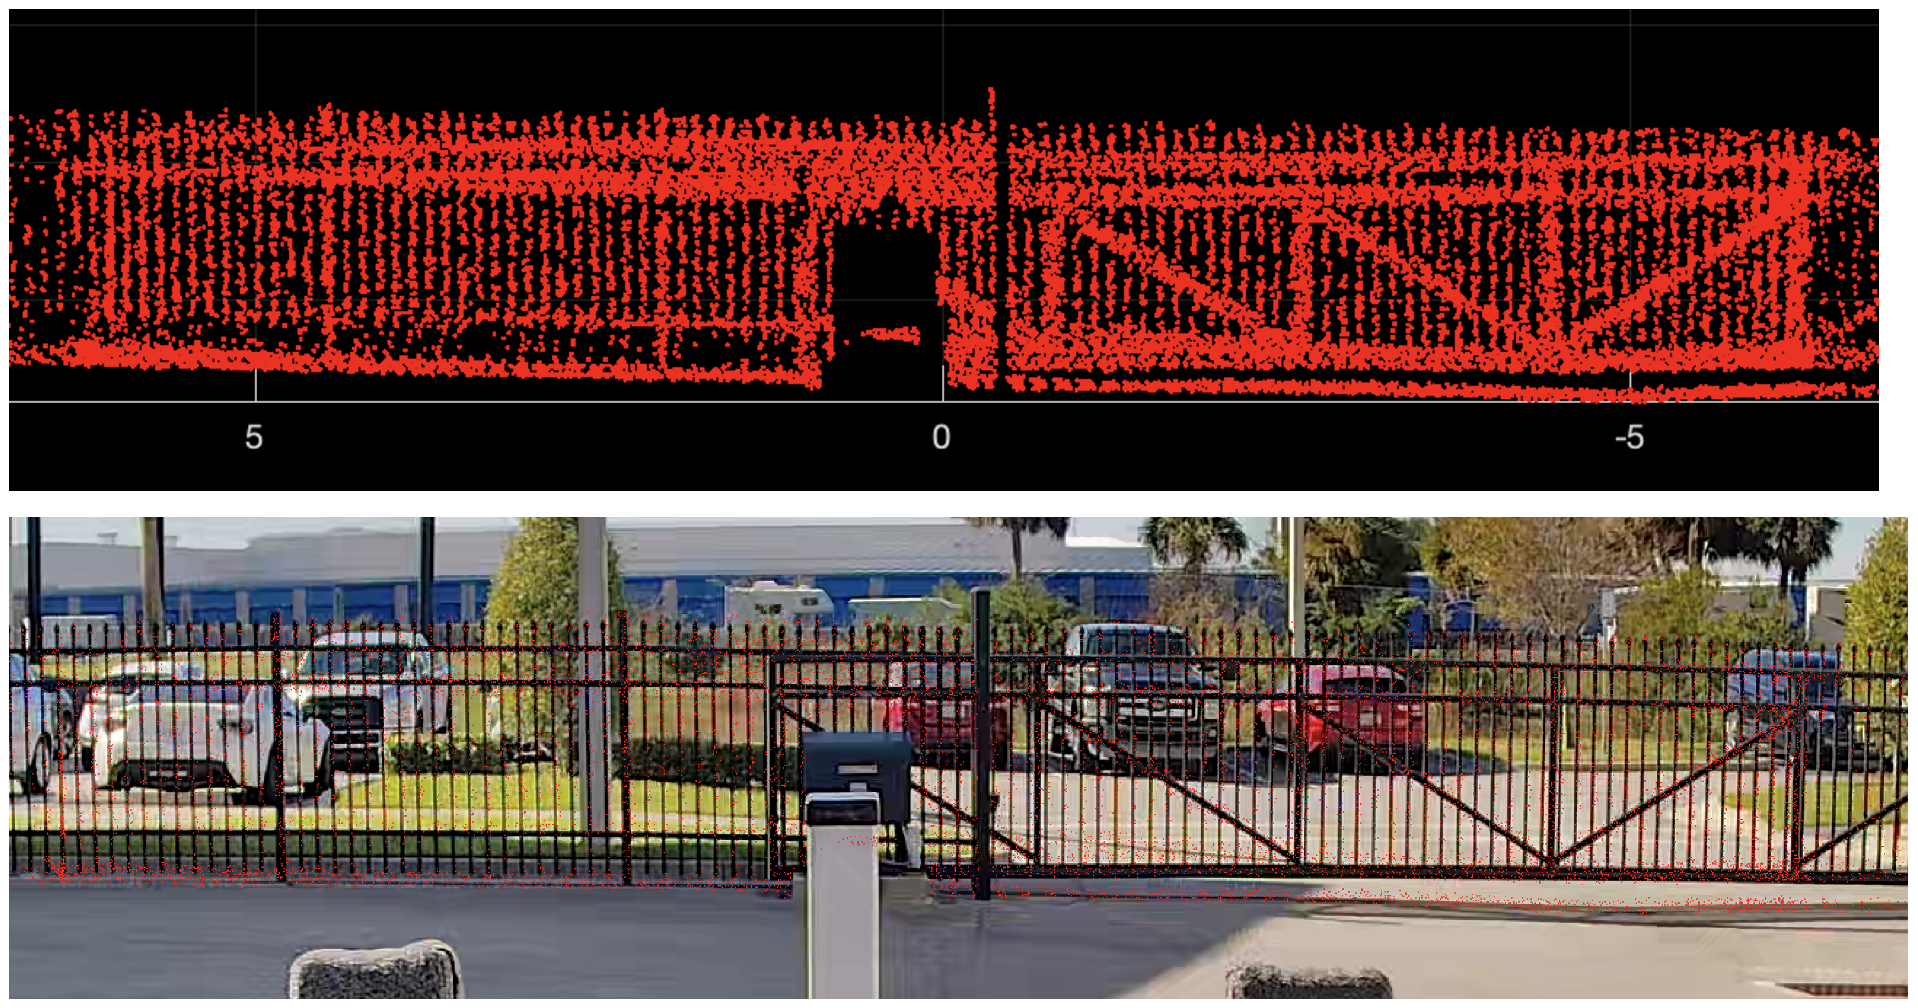
\includegraphics[width=0.94\linewidth]{Images/LiDAR_calib_fence.png}
    \caption{}
\end{subfigure}
\caption{Vertical (red) and horizontal (green) macro-level features within the point cloud (a) are isolated (b) to support visual refinement of the camera–LiDAR alignment.}
\end{figure}

\begin{figure}[ht]
    \centering
    \includegraphics[width=0.8\linewidth]{Images/LiDAR_overlay4.png}
    \caption{Initial calibration result showing early ROI-based alignment with overlaid geometric guides for evaluation.}
    \label{fig:LiDAR_overlay4}
\end{figure}
\begin{figure}[htp]
\begin{subfigure}{\textwidth}
\centering
\includegraphics[width=0.94\linewidth]{Images/LiDAR_overlay3A.png}
    \caption{Three isolated regions of interest (ROI) in the LiDAR point cloud.}
    \label{fig:LiDAR_overlay3A}
\end{subfigure}
\bigskip
\begin{subfigure}{\textwidth}
\centering
\includegraphics[width=0.94\linewidth]{Images/LiDAR_overlay3B.png}
    \caption{}
    \label{fig:LiDAR_overlay3B.png}
\end{subfigure}
\caption{Final camera–LiDAR calibration. LiDAR ROIs containing identifiable geometry (a) are projected as red pixels onto the HDR image (b) to confirm alignment quality.}
\label{HDR_calib_final}
\end{figure}
%%%%%%%%%%%%%%%%%%%%%%%%%%%%%%%%%%%%%%%%%%%%%%%%%%%%%%%%%%%%%%%%%%%%
\subsection{Temporal Calibration}
\label{time_sync}

This section discusses how each of the distributed computers and sensor are kept in sync with each other.
% Section \ref{comp:network} discussed the network architecture onboard the Minion \ac{USV} and dealt with the concept of network latency.
Section \ref{time_sync_lan} discusses how a master clock time from the GPS is distributed throughout the network, and section \ref{time_sync_cam} discusses how camera data is transferred from one machine to another without loss of timing information.
It is important to note that the temporal offsets discussed here should not be affected by the network latency described in Section~\ref{comp:network}, as timing information is transmitted with the data, and not subject to how long it takes to be delivered. 

% Latency is used to describe the discrepancy between two system clocks as well as the delay experienced in data transmission over the \ac{LAN}.
% Offset is used to discuss the difference in time between sensor data timestamps.

% an offset between system clocks, referred to here as latency, and a discrepancy between the recorded timestamps within the camera and LiDAR sensor data 

Multi-modal sensor fusion for object detection fundamentally requires precise temporal alignment between sensors operating on independent clocks and sampling at different rates.  
For example, if two sensors are offset by 200 milliseconds while observing a vessel moving at $5~\mathrm{m/s}$ and located 30~m from the platform, their detections would appear approximately $1~\mathrm{m}$ apart—equivalent to nearly $2^{\circ}$ of angular separation in the field of view.  
Such a discrepancy disrupts the spatial alignment between LiDAR points and image features, emphasizing the importance of consistent timing across all data streams.
While an inter-sensor offset of 20 milliseconds or less would ensure that collected data is within the tolerance of our detection system in a real-world scenario, this level of precision was determined to be unnecessary for the RobotX competition and was relaxed to 100 milliseconds.

% In maritime applications, where vehicle motion is relatively slow compared to ground-based platforms, sub-millisecond synchronization is generally unnecessary.  
% For the same vessel traveling at $5~\mathrm{m/s}$ and 30~m range, a temporal offset of $20~\mathrm{ms}$ limits apparent displacement to about 0.1~m, corresponding to less than two pixels in the downsampled image used for YOLO-based detection.  
% As demonstrated in Chapter~\ref{realtime_object_detection}, this level of alignment provides sufficient temporal accuracy for late-fusion operations.
% Therefore, a 20~ms offset is adopted as the maximum allowable synchronization error for this system.
% In this work, the design requirement is an inter-sensor clock \emph{offset} of $\leq 20~\mathrm{ms}$, which limits apparent target displacement to $\approx 0.1~\mathrm{m}$ at 30~m for a vessel moving at $5~\mathrm{m/s}$.  
% Note that offset (clock difference between devices) is distinct from end-to-end video latency (capture→decode delay); latency does not break fusion when frame timestamps are preserved.

% The next subsections describe the timing architecture: network synchronization across the vessel, Network Time Protocol for millisecond alignment of compute nodes, Precision Time Protocol for microsecond alignment of LiDAR units, and camera synchronization with timestamps embedded in the video bitstream and recovered at the receiver. Final timing performance and any corrective alignment used for LiDAR fusion are reported in Sec.~\ref{sec:time_sync_results}.


% Offset is the difference between device clocks at the same instant in time. 
% It shifts timestamps and creates apparent motion between modalities. 
% Latency is the delay from image exposure to availability at the receiver. Latency changes throughput but not the recorded capture time when timestamps are preserved. 
% At 5~m/s and 30~m range, a 20~milliseconds offset yields about 0.1~m apparent displacement, which is acceptable for late fusion. 
% The next subsections describe network synchronization, NTP for millisecond alignment of compute nodes, PTP for microsecond alignment of LiDAR units, and camera time-stamping within the video bitstream. Final offset and pipeline latency measurements appear in Section ~\ref{time_sync}.
% \textcolor{red}{This needs revision. The next section discusses latency, which needs to be identified as a separate measure from offset. Redo this last paragraph to correct.}

%%%%%%%%%%%%%%%%%%%%%%%%%%%%
\subsubsection{Network Synchronization} \label{time_sync_lan}

The Minion platform employs a hierarchical time synchronization architecture that distributes GPS-disciplined time from the PinPoint receiver to all perception sensors.
% \textcolor{blue}{achieving millisecond-level accuracy for camera observations and microsecond-level synchronization for LiDAR measurements. } 
In this configuration, the GPS clock serves as the master time source, which is distributed over the network via \ac{NTP} for coarse alignment or \ac{PTP} to achieve higher precision.
Together, these layers establish a unified temporal framework supporting reliable cross-modal data fusion and performance evaluation.

The synchronization hierarchy cascades timing information from the PinPoint GPS receiver, through the Atlas computing cluster, to the Jetson Xavier in the camera enclosure, and finally to each Livox Horizon LiDAR unit. This hierarchy is intentionally structured to align with the system’s physical and logical topology:

% PinPoint GPS → Atlas PC (Chrony NTP server) → Jetson Xavier (NTP client, PTP master) → Livox Horizon LiDAR (PTP clients)

At the top of this chain, the PinPoint GPS module provides Coordinated Universal Time (UTC) with sub-microsecond accuracy using the Global Navigation Satellite System (GNSS) signal. This external clock acts as the authoritative reference for the entire vessel, ensuring that all downstream systems inherit a consistent time base independent of internet connectivity.

%%%%%%%%%%%%%%%%%%%%%%%%%%%%
% \subsubsection{Network Time Protocol} \label{NTP}
% \paragraph{NTP}
Within the local area network (LAN), the Chrony \ac{NTP} daemon runs on the primary Atlas computer, which serves as the authoritative time server for all onboard devices. Chrony continuously disciplines the system clock using the GPS reference and corrects for minor drift caused by oscillator instability.

The NVIDIA Jetson AGX Xavier inside the camera enclosure operates as an \ac{NTP} client, synchronizing its system clock with the Atlas PC over the local Ethernet link. The resulting clock alignment achieves approximately 1–10~milliseconds accuracy—sufficient for coordinating 10~Hz camera streams and maintaining consistent ROS timestamps across computing nodes.

The synchronization status is verified at startup by onboard scripts that query Chrony before any video or LiDAR processes begin. This verification ensures that recording never proceeds with unsynchronized clocks. In addition, automated diagnostic checks allow operators to confirm that time distribution remains stable throughout offshore missions, where the GPS link represents the sole external time authority

%%%%%%%%%%%%%%%%%%%%%%%%%%%%
% \subsubsection{Precision Time Protocol} \label{PTP}
% \paragraph{PTP}
While \ac{NTP} provides millisecond-level precision for cameras and computing nodes, LiDAR sensors demand tighter synchronization. Each Livox Horizon operates at 100~Hz with microsecond-timestamped measurements, where even millisecond-level drift would cause measurable spatial distortion during vessel motion. To meet this requirement, the Jetson Xavier distributes the \ac{PTP} signal using the Linux ptp4l service.

In this configuration, the Jetson acts as the \ac{PTP} master clock, broadcasting timing packets over the camera-enclosure network to all three Livox devices, which function as \ac{PTP} slaves. \ac{PTP} uses hardware-timestamped Ethernet packets to measure network delay symmetrically and correct for it in real time, achieving sub-microsecond synchronization between LiDAR units. The Livox Viewer utility confirms synchronization state during system startup, and visual indicators within the GUI report “active 1588 signal” once synchronization is established.

\begin{figure}[htbp]
\centering
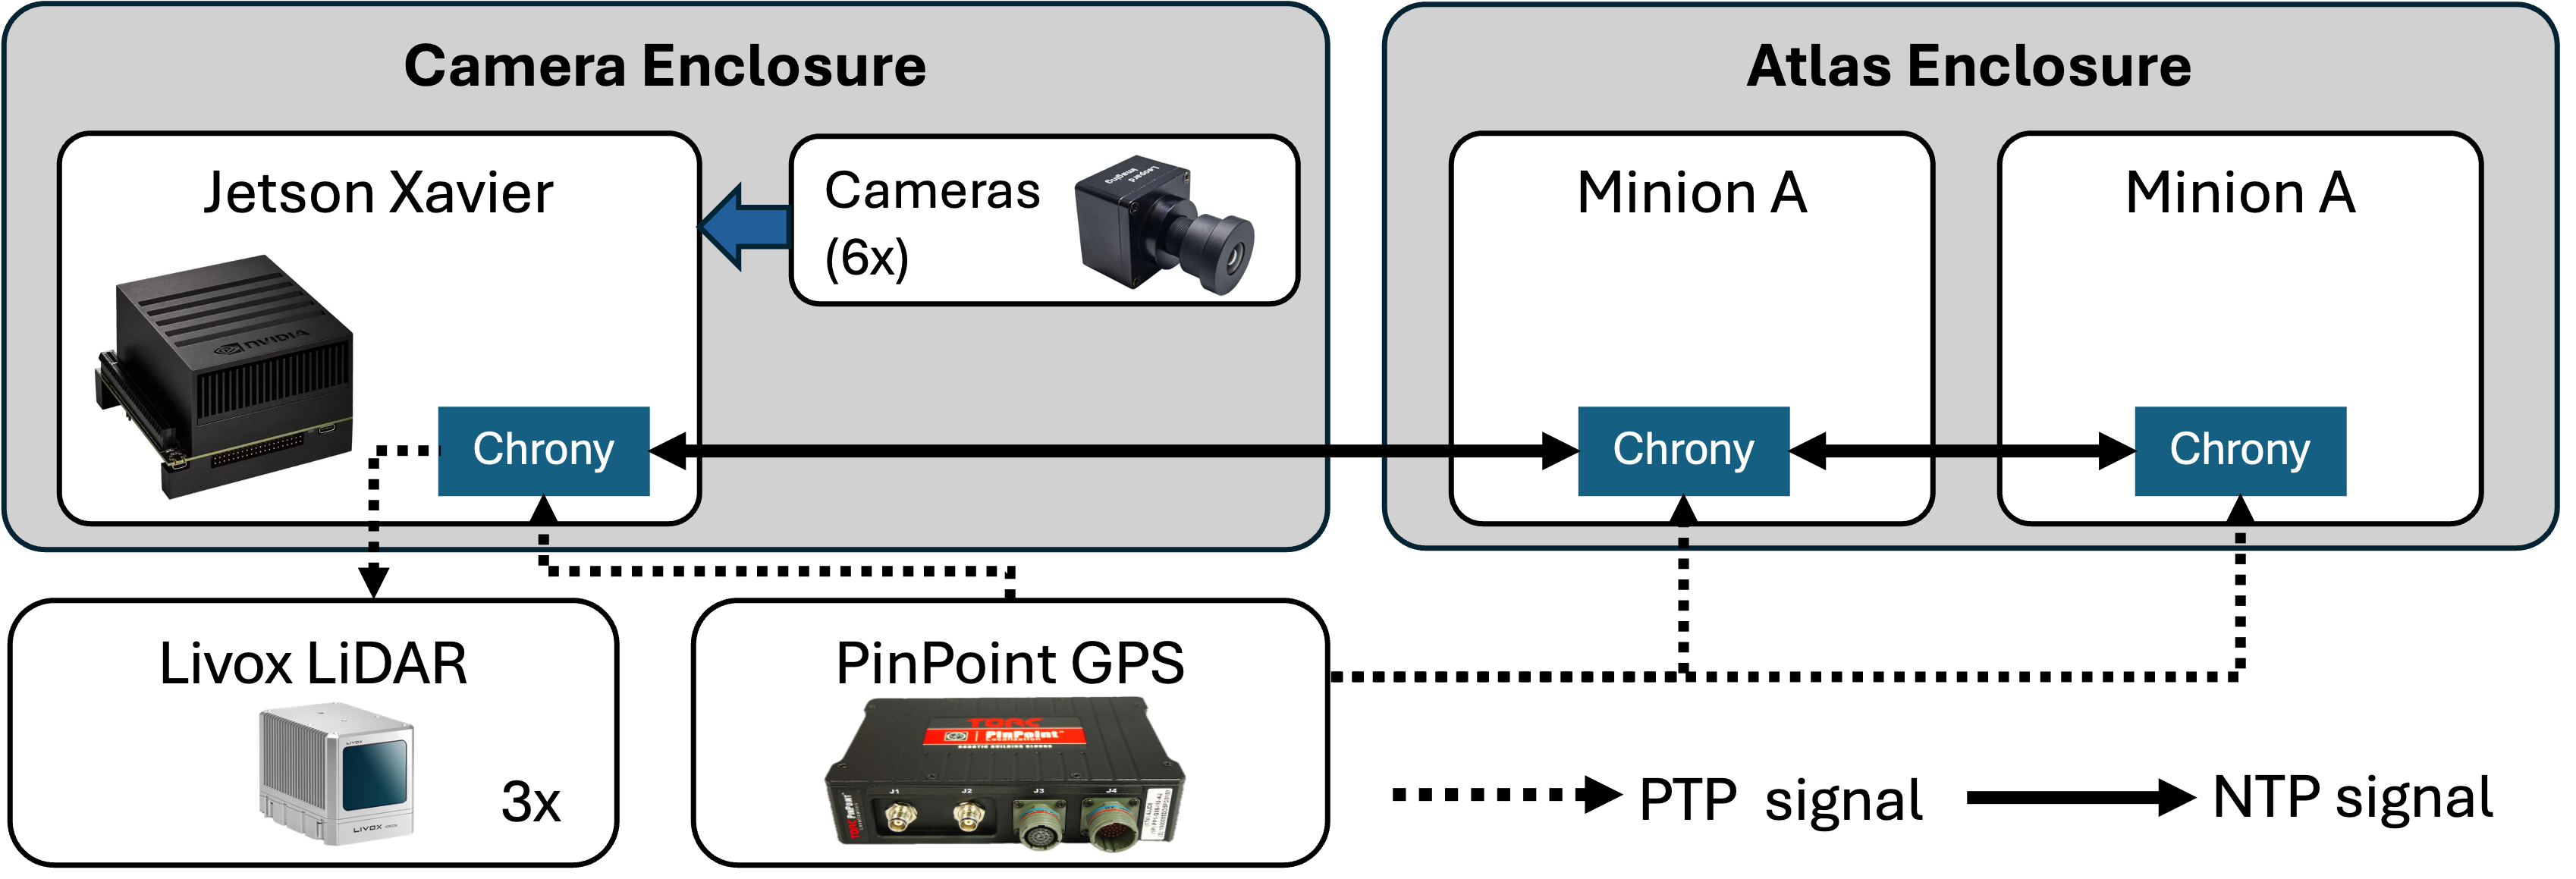
\includegraphics[width=0.8\textwidth]{Images/NTP.png}
\caption{LAN diagram for Minion USV}
\label{fig:network_sync}
\end{figure}

%%%%%%%%%%%%%%%%%%%%%%%%%%%%%%%%%%%%%%%%%%%%%%%%%%%%%%%%%%%%%%%%%%%%
\subsubsection{Camera Synchronization} \label{time_sync_cam}

Accurate video timestamps are essential for aligning image data with LiDAR point clouds. To achieve frame-level temporal precision, the Minion system embeds timestamps directly into the H.264/H.265 video stream generated by the Jetson Xavier using the GStreamer framework. This ensures that timing information remains synchronized with the frame itself, surviving compression, transmission, and playback.

% \paragraph{prior solution}
% Earlier implementations of the Minion perception system—originally developed by Thompson~\cite{thompson2023} employed a custom GStreamer plugin that performed two timestamping operations.
% First, it generated an adjacent .csv file containing timestamps that aligned to each frame of locally recorded video; second, it embedded the same timestamps into the closed-caption (CEA-608) layer of the \ac{RTSP} video stream.
% While this method was effective for offline data processing using the locally saved video files, the video stream is conducted asynchronously, and the RTSP protocol is unable to keep the closed-caption stream data linked to video frames.
% This limitation motivated the development of an \ac{SEI}-based synchronization method described below.
Earlier implementations of the Minion perception system—originally developed by Thompson~\cite{thompson2023}—employed a custom GStreamer plugin that performed two time-stamping operations. 
First, it generated an adjacent .csv file containing timestamps aligned to each frame of the locally recorded video. 
Second, it embedded the same timestamps into the closed-caption (CEA-608) layer of the \ac{RTSP} video stream. 
While effective for offline data processing using the saved video files, this method was limited by the asynchronous nature of \ac{RTSP}, which cannot maintain a persistent link between closed-caption data and video frames. 
This limitation motivated the development of the \ac{SEI}-based synchronization method described below.

% \paragraph{developed solution}

The current implementation replaces the caption-based approach with direct timestamp embedding using Supplemental Enhancement Information (SEI) Network Abstraction Layer (NAL) units defined in the H.264/H.265 standard.
Each video frame receives a GPS-disciplined system timestamp at the instant of capture from the camera sensor. These timestamps are stored as 64-bit values (milliseconds since Unix epoch) and attached to each frame via a custom GStreamer extension. % (CustomTimestampMeta).
This method keeps the timestamp data inextricably linked to the same video layer that is transmitted over \ac{RTSP}, guaranteeing that each video frame received will have a timestamp, even if dropped frames are experienced.
The complete video processing pipeline is visualized as a block diagram in Figure \ref{video_pipeline}.

% During encoding, a pad probe inserts the SEI NAL units immediately before the RTP payload (rtph264pay), ensuring that every encoded frame carries its own timestamp embedded within the bitstream.
% Because this method fits within the encoding standard, the timestamps persist through compression and streaming, which eliminates the complexity of the prior approach and maintains compatibility with all conventional video decoders.

\begin{figure}[htbp]
\centering
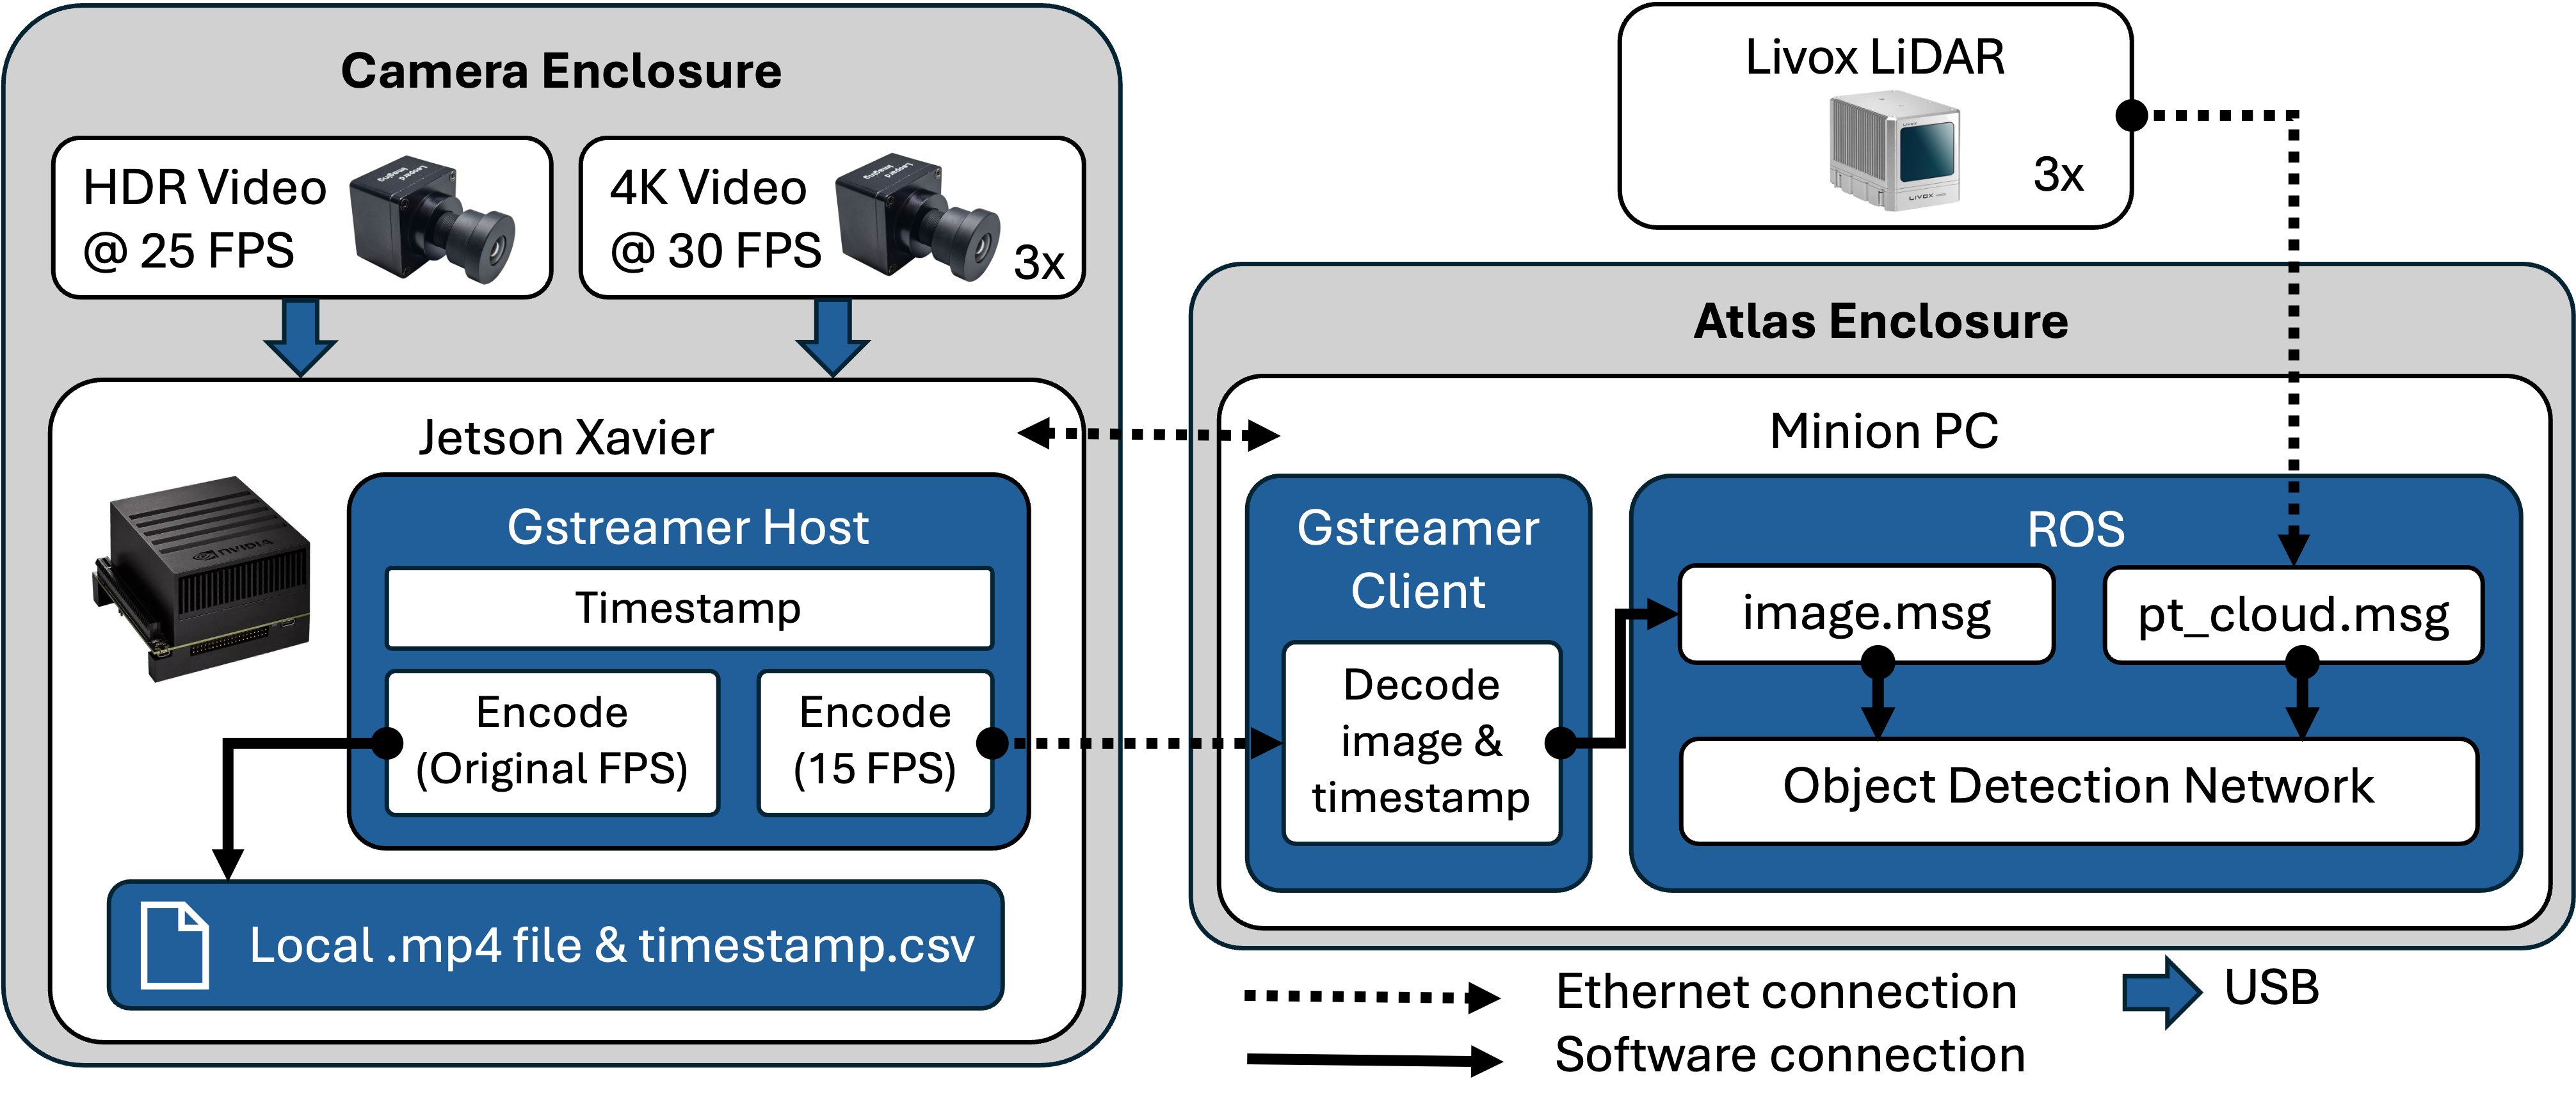
\includegraphics[width=0.8\textwidth]{Images/Block_Diagram.png}
\caption{LAN diagram for Minion USV}
\label{fig:sensor_block_diagram}
\end{figure}



% v4l2src → videoconvert → videorate → x264enc → [SEI insertion] → rtph264pay → RTSP stream

% Captured video at 2880×1860px and 60fps is downsampled to 10fps for transmission, balancing temporal resolution with network bandwidth. The SEI timestamp metadata is attached prior to frame-rate conversion, ensuring that each output frame retains its original capture time.
% The pipeline is fully compliant with ITU-TH.264 Annex~D and has been verified for compatibility with both H.264 and H.265 encoders.

At the receiving end, the Atlas PC decodes incoming streams using a complementary GStreamer pipeline equipped with a pad probe on the \texttt{h264parse} element. This probe identifies SEI NAL units and extracts the embedded timestamp payload before decoding. The recovered timestamps are then written to the ROS message headers of the corresponding image frames via the \texttt{image\_transport} framework.


\begin{figure}[htbp]
\centering
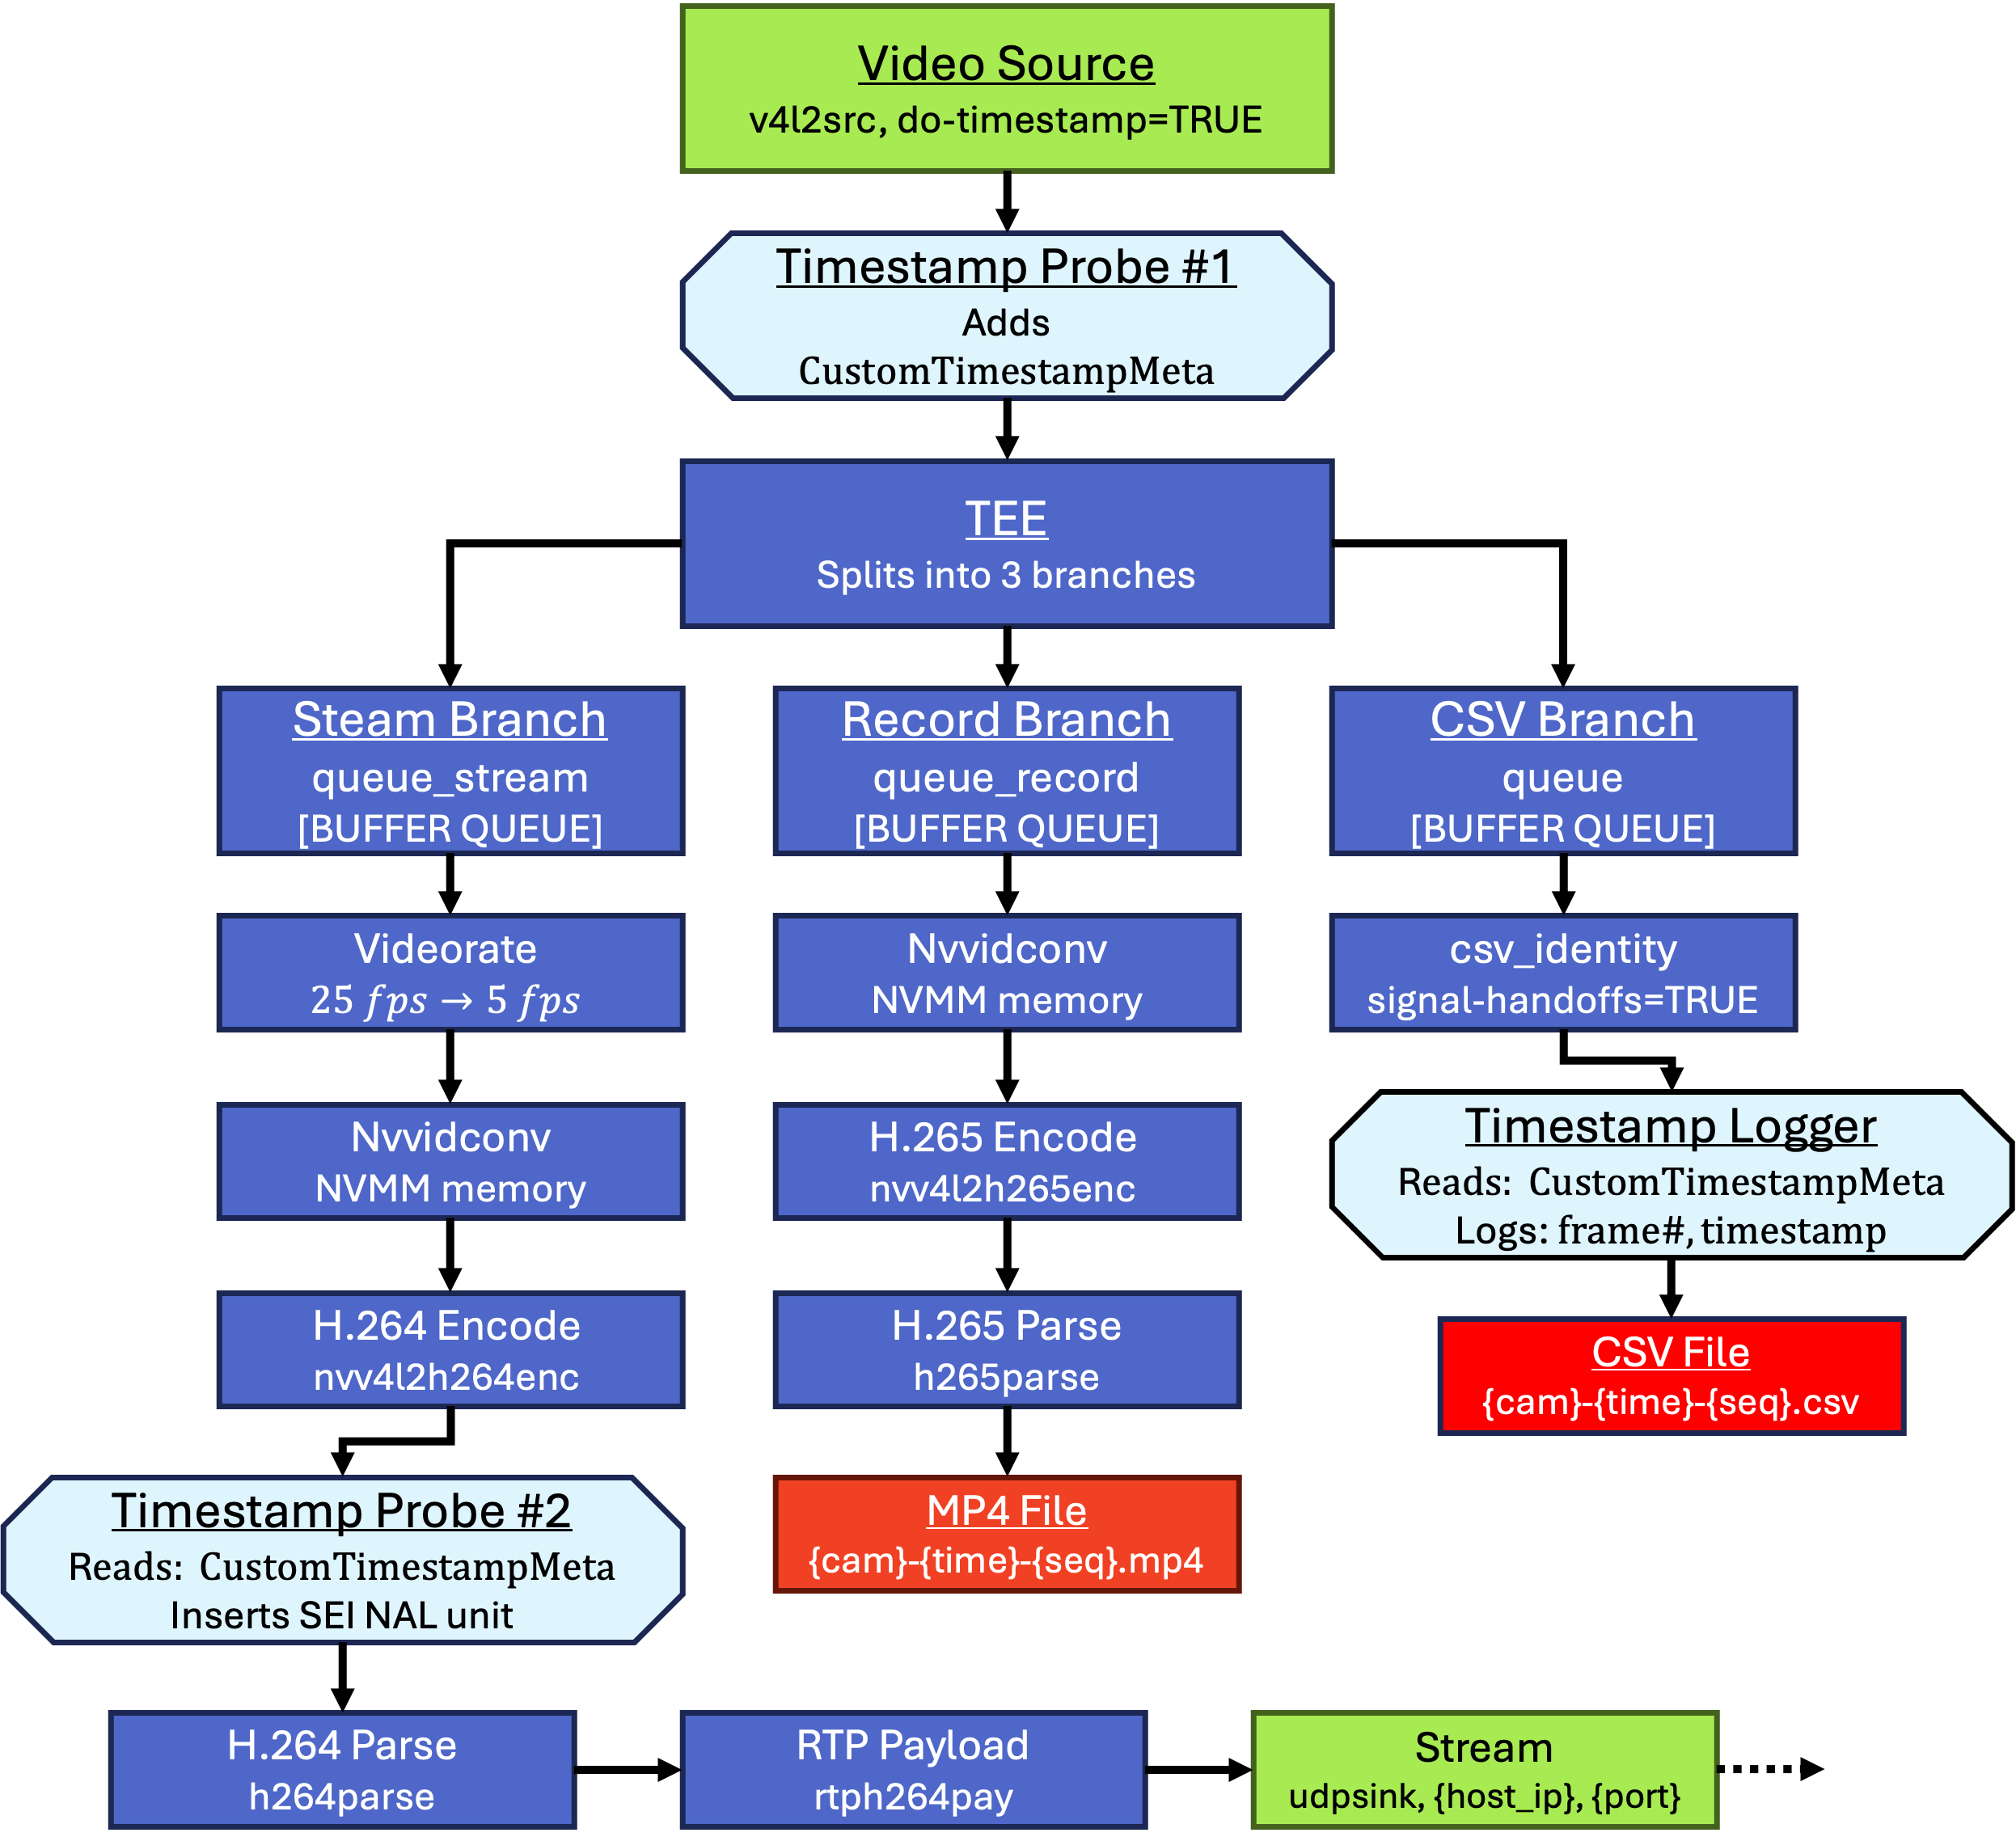
\includegraphics[width=5in]{Images/gstreamer_block.png}
\caption{Block diagram of the NVIDIA Jetson's video pipeline. Green rectangles represent video data entering or leaving the pipeline, while red rectangles indicate local file creation. Light-blue rectangles with chamfered corners denote timestamp acquisition and application operations within the pipeline.}
\label{video_pipeline}
\end{figure}
%%%%%%%%%%%%%%%%%%%%%%%%%%%%%%%%%%%%%%%%%%%%%%%%%%%%%%%%
\subsection{Results: Temporal Synchronization} \label{results)time_sync_cam}

An initial evaluation of the video stream and time-stamping system was conducted under conditions that simulated expected network load conditions.
Video data was recorded for 14.5 seconds at 10 \ac{fps} (twice the anticipated operational rate) for a total of 8,720 frames. 
The NVIDIA computer in the camera enclosure was accessed via SSH terminal and displayed a log of each timestamp being recorded and sent over the RTSP video stream. 
Similarly, the Atlas PC was connected to via SSH and displayed the timestamp being received over the RTSP video stream.
This data was also logged in a text file on the respective machines and compared for analysis. 
To ensure real-world clock precision, a real-time clock was set up in front of the camera displaying the current time, and transmitted as the subject of the video feed. An image of this setup is presented in Figure~\ref{fig:time_sync1}
This allows for any internal clock drift to easily be identified by comparing the transmitted timestamp to the time displayed in the video itself.

\begin{figure}[htbp]
    \centering
    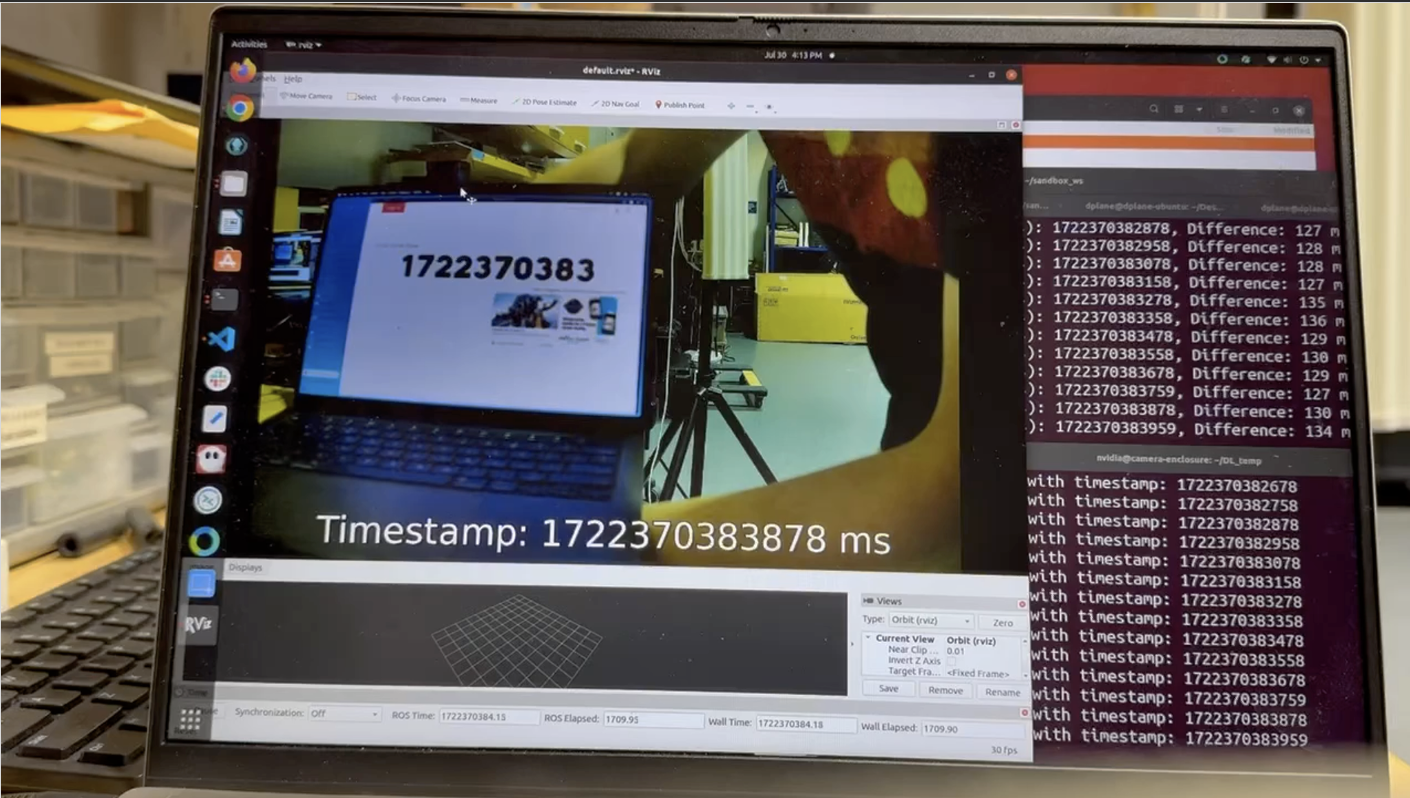
\includegraphics[width=0.8\linewidth]{Images/time_sync1.png}
    \caption{Testing the timestamp embedding within the RTSP stream for dropped frames and real-world temporal accuracy.}
    \label{fig:time_sync1}
\end{figure}
% Data was recorded by outputting the timestamps being sent and received by video camera, as well as by exporting this data to a log file on each machine. 

During the test, system-wide clock synchronization was measured using Chrony, which reported an average offset of $197;\text{ms};\pm;33;\text{ms}$ between the NVIDIA Jetson and Atlas machines.
The results of this test showed a total delay in video frame reception of 127 milliseconds, and logs between computers showed zero dropped frames with a 100\% match between timestamps.
\textcolor{blue}{This test was performed on Helios - Not Atlas, and did not have a true "master clock", if I recall. Find more recent test data. I would bet that running with updated chrony and ptp4l settings reduces this number significantly.}

Despite this result in frame delivery and timestamp assignment during testing, analysis of the recorded ROS bagfile data revealed a measurable drift between the original frame timestamps on the Jetson and those recorded by the Atlas system. 
% This discrepancy is believed to stem from thermal issues within the camera enclosure that were encountered during data collection.
% Therefore, some postprocessing of the data was required to ensure its validity.
This discrepancy is believed to result from thermal effects within the sealed camera enclosure during extended operation. 
Although no direct temperature measurements were recorded during this test, subsequent observations suggest that overheating may influence the Jetson's internal clock stability. 
This hypothesis remains unverified and will be revisited in Section~\ref{recommendations}.

To resolve this, structural similarity (SSIM) scoring was employed to match each frame recorded by ROS on the Atlas to its corresponding source frame from the original video files on the Jetson. 
Although SSIM is conventionally used to assess visual degradation from compression, in this context, it served as a frame-matching metric: matched frames produced SSIM scores near 1.0, while mismatches scored closer to 0.0. The SSIM metric used is defined as:
\begin{equation}
    \text{SSIM}(x, y) = \frac{(2\mu_x\mu_y + C_1)(2\sigma_{xy} + C_2)}{(\mu_x^2 + \mu_y^2 + C_1)(\sigma_x^2 + \sigma_y^2 + C_2)}
\end{equation}

In this expression, $\mu_x$ and $\mu_y$ represent the mean pixel intensities of images $x$ and $y$, $\sigma_x^2$ and $\sigma_y^2$ are their variances, $\sigma_{xy}$ is the covariance between the images, and $C_1$ and $C_2$ are small constants that stabilize the division when the denominator is near zero.

To initialize alignment for each bag file, the first five ROS image messages within each bag were manually paired to the corresponding frames in the source video.
This established the offset the system was experiencing at the time the data was being recorded, which was then used to programmatically pair the remaining image messages in the bag with their video frame counterparts.
SSIM-based alignment was then automated on a subset of frames sampled at one-second intervals across each bagfile. 
Once alignment was confirmed through SSIM scores, the timestamps and frame indices for the intermediate frames were interpolated from the verified matches. 
Accordingly, the total number of frames analyzed by SSIM is approximately equal to the total number of seconds of recorded data.

To streamline this process across all 112 recorded bag files, a database was created to store file names, paths, and relevant metadata, allowing image and video data to be easily cross-referenced between the video and CSV files, and more than 100,000 ROS image messages. 
The same database also served as the repository for SSIM scores, interpolated matched frame numbers, and both the original and corrected timestamps for each image message. 
This dual-purpose design enabled automation of the SSIM alignment process while simultaneously providing a complete record of the aligned frame data for offline analysis and validation.

%%%%%%%%%%%%%%%%%%%%%%%%%%%%%%%%%%%%%%%%%%%%%%%%%%%%%%%%%%%%%%%%%%%%
%%%%%%%%%%%%%%%%%%%%%%%%%%%%%%%%%%%%%%%%%%%%%%%%%%%%%%%%%%%%%%
\section{Sensor Data and Dataset}
\label{sec:sensor_data_dataset}

% This section describes the multimodal data produced by the Minion sensing platform, 
% the \ac{ROS}-based framework used for data acquisition and synchronization, 
% and the construction of the dataset used for training and evaluating perception algorithms.
% Together, these processes establish the bridge between hardware-level sensing and 
% machine-learning-based object detection methods discussed in Chapter~\ref{realtime_object_detection}.

This section describes the collected sensor data, the ROS node architecture used to record it, 
and the organization of the resulting dataset used throughout this research.  
It integrates over three hours of multi-sensor maritime data collected aboard the Minion between October 2023 and May 2025.

The resulting dataset represents a multi-modal maritime perception package that integrates synchronized LiDAR, HDR video, GPS, and IMU data collected under real-world conditions, and is structured to enable rapid offline reproduction of real-time detection and fusion results.


%%%%%%%%%%%%%%%%%%%%%%%%%%%%%%%%%%%%%%%%%%%%%%%%%%%%%%%%%%%%%%
\subsection{ROS Node Architecture for Data Collection}
\label{sec:ros_architecture}

Data were collected using the ROS 1 \texttt{Noetic} framework on Ubuntu 20.04, 
leveraging custom C++ packages developed for LiDAR–camera fusion and object detection.  
% Figure \ref{fig:ros} outlines the software architecture.  
ROS 1 Noetic was selected because the Minion software stack had not yet been fully migrated or validated under ROS 2, while the ROS 1 implementation was stable, field-tested, and fully operational across all sensing subsystems.

Raw data from the Pinpoint GPS, Livox LiDAR units, and the RTSP video stream are converted into individual ROS messages through separate ROS nodes and published to sensor-specific topics as visualized in Figure \ref{fig:ros}.  
Temporal synchronization was achieved by applying original hardware timestamps to each ROS message header: LiDAR packets were time-stamped by the Livox\_SDK driver, while the RTSP video stream was decoded frame-by-frame, with timing extracted from H.264 metadata and applied to each image message before publication, as detailed in Section~\ref{time_sync_cam}.

All sensor topics were recorded using the standard rosbag record utility without compression. 
The resulting bag files constitute the dataset itself, recorded in real-time during field operations and later parsed offline for analysis and model training.



% \subsubsection{LiDAR Pipeline}  
% Four nodes implemented object detection, filtering, and 3-D clustering.  
% The \texttt{fusing\_node} merged multiple Livox point clouds into a unified global frame, 
% and \texttt{point\_cloud\_module\_node} applied occupancy-grid mapping and DBSCAN clustering with multivariate-Gaussian (MVG) classification.  
% Typical update rates were 5 Hz for LiDAR and 10 Hz for vision nodes.  

\begin{figure}[htbp]
    \centering
    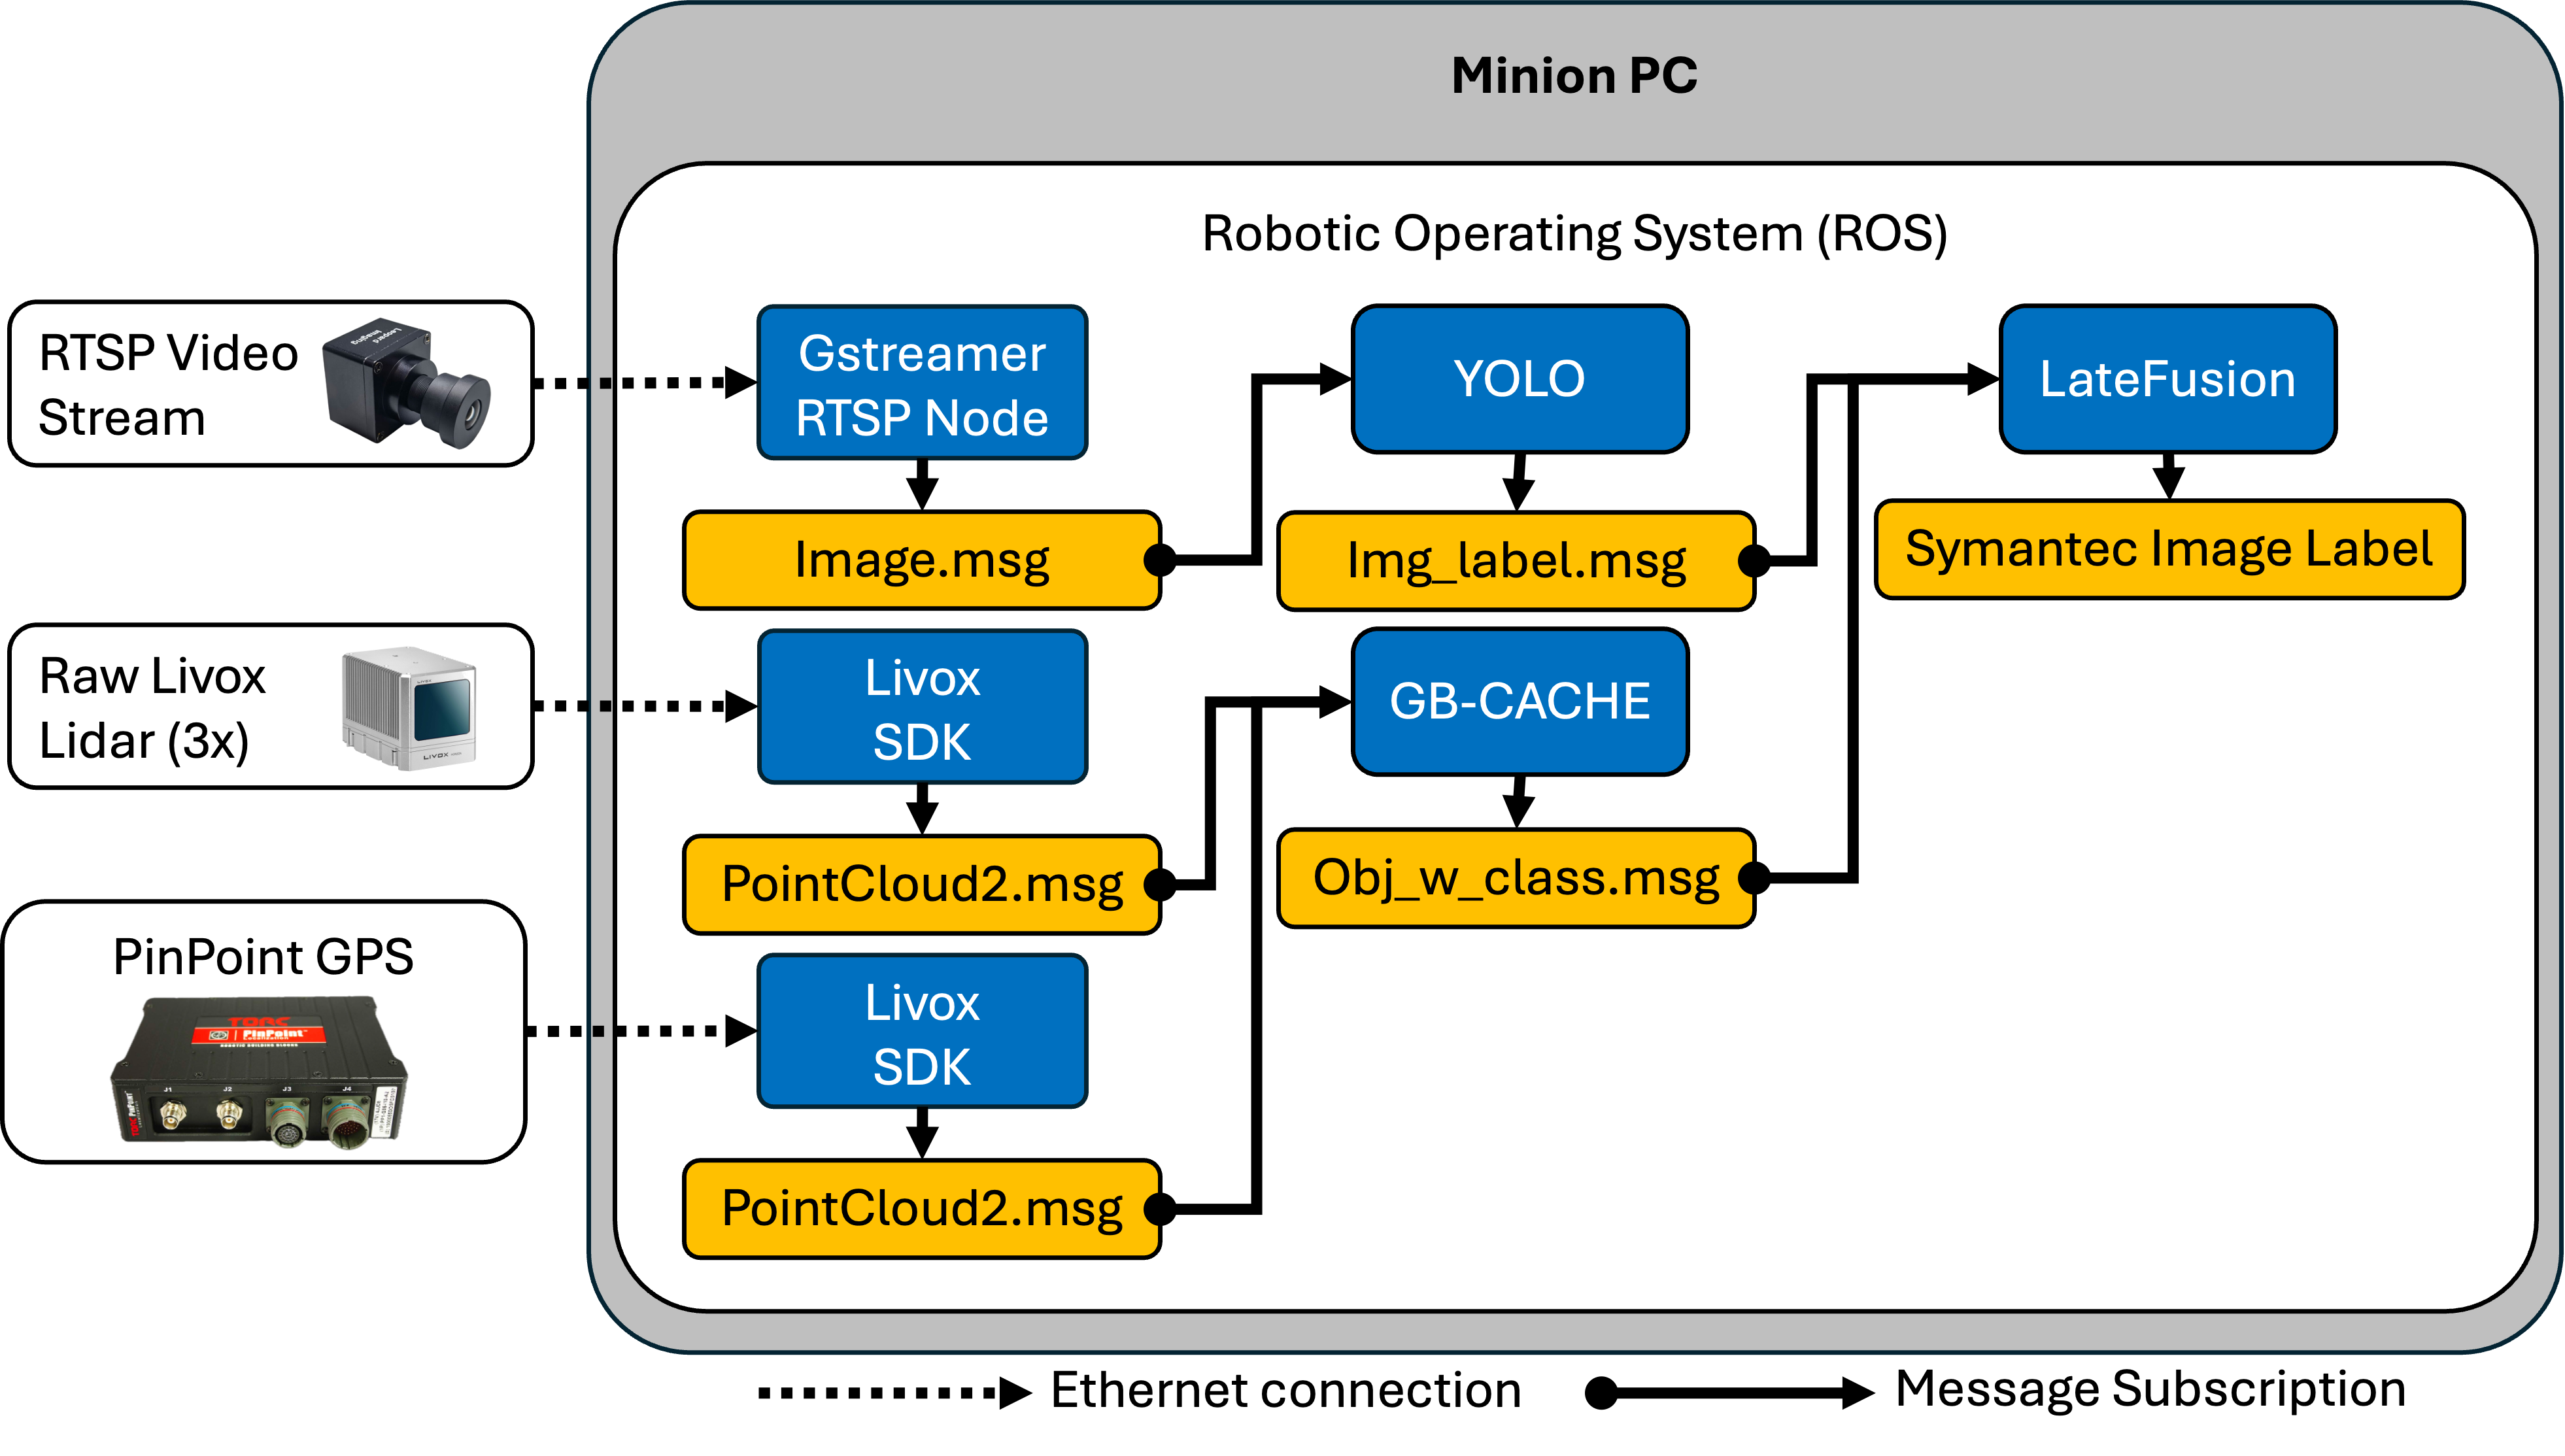
\includegraphics[width=0.95\linewidth]{Images/ros.png}
    \caption{Software architecture used to acquire synchronized LiDAR, HDR video, GPS, and IMU data within the ROS 1 Noetic framework. Each node publishes time-stamped sensor messages to modality-specific topics, allowing for the raw data to be played back with accurate timing.}
    \label{fig:ros}
\end{figure}



%%%%%%%%%%%%%%%%%%%%%%%%%%%%%%%%%%%%%%%%%%%%%%%%%%%%%%%%%%%%%%
\subsection{Data Collection Overview}
\label{sec:data_overview}

The data collection framework was deployed aboard Minion across multiple field days before, during, and after the RobotX Competition, producing the complete dataset used in this research.
A total of 122 ROS bag files were recorded over 13 collection days,  containing more than 52 million sensor messages and 3.67 hours of synchronized data.
Across all campaigns, the dataset includes approximately 132,000 camera frames and 66,000 LiDAR scans, corresponding to an average of about 10,000 frames per collection day.
Tables \ref{tab:rosbag_stats} and \ref{tab:obj_class_dets} aggregate these statistics.  
HDR messages correspond to the total number of image-topic messages recorded, and LiDAR message counts can be estimated as the total recorded duration multiplied by 300 messages per second (three sensors operating at 100 Hz each).
Based on the total durations of recorded bagfiles, this equates to more than 3.9 million LiDAR frames per unit and more than 11 million LiDAR messages when combined.

\begin{table}[htbp]
\centering
\begin{tabular}{llrrr}
\hline
\multicolumn{2}{c}{Collection Period} & Bags & HDR Messages & Seconds \\
\hline
\hline
Competition Training & Sep 22 - Oct 26, 2024 & 29 & 8,408,242 & 2,145 \\
RobotX Competition & Nov 3 - Nov 9, 2024 & 62 & 33,336,777 & 8,026 \\
Summer 2025  & May 29, 2025 & 31 & 10,488,090 & 3,010 \\
\hline
\textbf{Total} & \textbf{---} & \textbf{122} & \textbf{52,233,109} & \textbf{13,181} \\
\hline
\end{tabular}
\caption{Overall data collection statistics for each campaign, showing the number of ROS bag files, total recorded messages, and total recording duration in seconds.}
\label{tab:rosbag_stats}
\end{table}

Peak collection occurred during November 2024 in preparation for the Maritime RobotX Challenge, with additional data gathered during Summer 2025 to expand environmental variety.  
Data collection was limited to favorable weather conditions to ensure team and equipment safety. 
All sessions were conducted under calm seas, low winds, and generally clear or partly cloudy skies, with no recordings made during inclement or low-visibility conditions.
Each recording included synchronized data from three Livox Horizon LiDARs  (\texttt{/livox/lidar\_front}, \texttt{/livox/lidar\_port}, and  \texttt{/livox/lidar\_starboard}), one Leopard Imaging HDR camera publishing  \texttt{/camera/image} and \texttt{/camera/info}, and the IMU and GPS topics defining the  \texttt{map\_to\_base\_link} and \texttt{base\_link\_to\_sensor} transforms.
For clarity, topic and sensor identifiers are presented here using descriptive names (e.g., \texttt{/livox/lidar\_front}), whereas the original recorded topics used serial-number-based identifiers corresponding to each LiDAR unit.


\begin{table}[ht]
\centering
\begin{tabular}{llll}
\hline
\multicolumn{4}{c}{Total Object Detections by Class}\\
\hline
\hline
Class & Class       & Num. Samples & Unique Objs \\
1     & Tall Buoy   & 266381       & 730         \\
2     & A2 Buoy     & 83583        & 674         \\
3     & A3 Buoy     & 69559        & 803         \\
5     & Light Tower & 13171        & 48          \\
7     & Kayak       & 1624         & 39          \\
8     & Jon Boat    & 7543         & 171         \\
11    & Sailboat    & 7617         & 140  \\      
\hline
\end{tabular}
\caption{Total object detections and unique object counts for each labeled maritime class within the processed dataset.}
\label{tab:obj_class_dets}
\end{table}

Unique objects correspond to persistent object IDs assigned by the mapping system, as described in Section~\ref{gbcache}.

\begin{table}[ht]
\centering
\begin{tabular}{cllcc}
\hline
Legacy ID & Legacy Label & YOLO Label & LiDAR Label  & Included \\
\hline
1  & Tall Buoy          & Tall Buoy              & Tall Buoy          & Yes \\
2  & A2 Buoy            & Round Buoy (merged)    & A2 Buoy            & Yes \\
3  & A3 Buoy            & Round Buoy (merged)    & A3 Buoy            & Yes \\
4  & A5  Buoy           & —                      & —                  & - \\
5  & Light Tower        & Light Tower            & Light Tower        & Yes \\
6  & Dock               & —                      & —                  & - \\
7  & Power Boat         & Jon Boat               & Jon Boat           & Yes \\
8  & Sailboat           & Sailboat               & Sailboat           & Yes \\
9  & Kayak              & —                      & —                  & - \\
10 & UAV\_SR    & —                      & —                  & - \\
11 & UAV\_Rep   & —                      & —                  & - \\
\hline
\end{tabular}
\caption{Modality-aware class mapping. YOLO merges A2/A3 into \emph{Round Buoy} because a single monocular image does not provide absolute scale; LiDAR retains A2 and A3 as distinct classes due to direct range measurements enabling size-based separation.}
\label{tab:class_map}
\end{table}

Metadata from each bagfile and associated video files, including topic names, message counts, and timestamps, were compiled into an SQLite3 database to support efficient indexing, retrieval, and temporal alignment tasks outlined in section~\ref{time_sync_cam}.
This dataset structure provides the foundation for the evaluation results presented in Section \ref{performance}. 

% %%%%%%%%%%%%%%%%%%%%%%%%%%%%%%%%%%%%%%%%%%%%%%%%%%%%%%%%%%%%%%
% \subsection{Data Organization and Processing}
% \label{sec:data_organization}

% The recorded dataset consists of multiple ROS topics operating at distinct rates. 
% The three Livox LiDAR sensors published point-cloud data at 100~Hz, the HDR camera produced image messages at 5~Hz, 
% and the combined GPS/IMU localization topics updated at approximately 5~Hz. 
% These asynchronous data streams were recorded concurrently into ROS bag files during field operations, forming the complete dataset used for subsequent analysis.

% All data were later reprocessed within ROS for operational testing and analysis. 
% Metadata from each bag file, including topic names, message counts, and timestamps, was extracted into an SQLite3 database 
% to support efficient indexing, retrieval, and temporal alignment tasks outlined in section~\ref{time_sync_cam}.
% This dataset structure provides the foundation for the training and evaluation results presented in Chapters~\ref{yolo} and~\ref{gbcache}. 
% The organization described here ensures that the models discussed in those chapters operate on a consistent, time-synchronized dataset, 
% allowing direct comparison of performance between the vision-only YOLO framework and the LiDAR-based GB-CACHE method.

% \paragraph{Temporal Synchronization}  
% Detailed discussion of temporal alignment and clock drift correction is provided in Section~\ref{time_sync_cam}. 
% Briefly, image and LiDAR frames were associated based on their recorded timestamps, ensuring that each pair represented 
% the closest available acquisition times within a latency bound of 50~ms.

% \paragraph{Spatial Registration}  
% Spatial alignment of LiDAR data to the camera frame use the extrinsic calibration derived in Section~\ref{sec:camera-lidar_results}. 
% Because the GPS/IMU topics operated at a lower rate than the LiDAR, the \texttt{robot\-localization} package within ROS interpolated position and heading between consecutive 5~Hz updates to generate intermediate pose estimates at 100~Hz. 
% These interpolated poses ensured each LiDAR scan was transformed using a temporally consistent platform orientation and position.


% %%%%%%%%%%%%%%%%%%%%%%%%%%%%%%%%%%%%%%%%%%%%%%%%%%%%%%%%%%%%%%
% \subsection{Dataset Construction for Machine Learning}
% \label{sec:dataset_construction}

% The processed dataset forms the basis for training and validating the vision and fusion models described in Chapters \ref{yolo} and \ref{gbcache}.  
% The dataset contains labeled maritime object classes, including navigation buoys, docks, vessels, and channel markers.  
% Each object instance includes a cropped RGB image (2880 × 1860 resized to 640 × 640 for network input), a corresponding LiDAR point subset in PCD format, a YOLO label file with normalized bounding boxes, and associated metadata such as timestamp, GPS pose, and lighting condition.

% The final YOLO training dataset consisted of 543 labeled images for training, 158 for validation, and 77 for testing. 
% Across all splits, the dataset contained 1,934 labeled objects with an average of 2.5 bounding boxes per image. 
% The class distribution was moderately imbalanced, with sailboats representing approximately 60\% of annotations, 
% followed by jon boats ($16$\%), tall buoys ($12$\%), light towers ($11$\%), and minor representation of round buoys and A3 markers ($<2$\%). 
% This class composition reflects the real-world frequency of visible maritime targets encountered during data collection.
% Training, validation, and test splits follow a 70 / 20 / 10 ratio, stratified by date to prevent temporal leakage between sets.

% The five YOLO class labels, tall\_buoy, round\_buoy, light\_tower, jon\_boat, and sailboat, correspond directly to the maritime object categories summarized in Tables~\ref{tab:obj_class_dets} and~\ref{tab:class_map}, with one key distinction. 
% While the LiDAR-based detection framework differentiates between A2- and A3-sized buoys as separate classes, these were combined into a single round\_buoy category for YOLO training because visual appearance alone does not reliably convey scale or distance. 
% As a result, the LiDAR models operate on six classes, whereas the YOLO models use five, excluding kayaks from both datasets due to insufficient representation for robust training.
%%%%%%%%%%%%%%%%%%%%%%%%%%%%%%%%%%%%%%%%%%%%%%%%%%%%%%%%%%%%%%
\subsection{YOLO Training Dataset}
\label{sec:yolo_training_data}

%%%%%%%%%%%%%%%%%%%%%%%%%%%%%%%%%%%%%%%%%%%%%%%%%%%%%%%%%%%%%%
% \subsection{Vision Dataset for YOLO Transfer Learning}
% \label{sec:vision_dataset_yolo}

A manually labeled image dataset was constructed to support the transfer learning and evaluation of the YOLO object detection network. 
All YOLO training images were obtained from video recorded directly on the Jetson.
Rosbag data was recorded intermittently, whereas the cameras operated and streamed continuously.
This ensured that a large pool of video data remained separate from the main dataset and available for YOLO training.

The complete dataset contained 778 annotated images with a total of 1934 labeled maritime objects from the six classes defined in Table \ref{tab:class_map} 
Each annotation was produced through a manual labeling process for objects present within each 2880 $\times$ 860 frame. 

The final dataset contained 778 annotated images and 1934 labeled maritime objects. 
Data were divided into training, validation, and test subsets following a 70:20:10 ratio.
Each subset preserved the relative class proportions observed in the complete dataset, which contained an average of 2.5 labeled objects per image across the five categories listed in Table~\ref{tab:class_map}.
The A2 and A3 buoy variants are virtually identical when viewed in isolation, as their size difference can only be inferred through comparison or with additional depth information in the image frame. 
Because YOLO operates purely on two-dimensional image data without access to spatial depth cues, there was no practical benefit to treating these as separate classes; both were therefore labeled collectively as \texttt{round\_buoy}.
\textcolor{blue}{Based on field observations, it is likely that A2 buoys were predominantly red, green, or blue, whereas A3 and larger buoys appeared black. 
However, since visually similar large black buoys were also observed throughout the rosbag dataset without verified size information, these classes were merged to maintain labeling consistency.}

\begin{table}[htbp]
\centering
\begin{tabular}{lccccccc}
\hline
Subset & Images & Labels & Tall Buoy & Round Buoy & Light Tower & Jon Boat & Sailboat \\
\hline
Train & 543 & 1,343 & 12.0\% & 1.4\% & 11.2\% & 15.8\% & 59.6\% \\
Validation & 158 & 390 & 14.1\% & 1.3\% & 13.1\% & 12.8\% & 58.7\% \\
Test & 77 & 201 & 16.4\% & 1.5\% & 9.5\% & 12.4\% & 59.7\% \\
\hline
Total & 778 & 1,934 &  &  &  &  &  \\
\hline
\end{tabular}
\caption{YOLO dataset composition and class distribution across training, validation, and test subsets.}
\label{table:yolo_data_split}
\end{table}

\noindent The relative consistency across all three subsets demonstrates that the temporal stratification preserved real-world object frequency while maintaining balance for training and evaluation. 
The test set was reserved exclusively for the final performance assessment described in Section~\ref{performance}.

%%%%%%%%%%%%%%%%%%%%%%%%%%%%%%%%%%%%%%%%%%%%%%%%%%%%%%%%%%%%%%
\subsection{GB-CACHE Training Dataset}
\label{sec:gbcache_training_data}

% \begin{figure}[htbp]
%     \centering
%     \includegraphics[width=0.9\linewidth]{Images/dataset_pipeline.pdf}
%     \caption{Processing pipeline from raw ROS bags to labeled training dataset.}
%     \label{fig:dataset_pipeline}
% \end{figure}

% This dataset structure provides the foundation for the training and evaluation results presented in Chapters~\ref{yolo} and~\ref{gbcache}. 
% The organization described here ensures that the models discussed in those chapters operate on a consistent, time-synchronized dataset, 
% allowing direct comparison of performance between the vision-only YOLO framework and the LiDAR-based GB-CACHE method.



%%%%%%%%%%%%%%%%%%%%%%%%%%%%%%%%%%%%%%%%%%%%%%%%%%%%%%%%%%%%%%%%%%%%
%%%%%%%%%%%%%%%%%%%%%%%%%%%%%%%%%%%%%%%%%%%%%%%%%%%%%%%%%%%%%%%%%%%%
%%%%%%%%%%%%%%%%%%%%%%%%%%%%%%%%%%%%%%%%%%%%%%%%%%%%%%%%%%%%%%%%%%%%
\chapter{Real-time Object Detection} \label{realtime_object_detection}

Real-time object detection lies at the core of autonomous perception, enabling vehicles to interpret their surroundings and respond safely to dynamic environments.
Effective detection requires identifying, classifying, and localizing objects rapidly enough to support decision-making and control loops, often under constraints of limited onboard computing and bandwidth.
In this work, these challenges are examined through vision and LiDAR detection pipelines implemented on the Minion sensing platform.

The central focus of this investigation is the development of a late-fusion framework that integrates information from both sensing domains to enhance detection robustness and confidence.
This framework represents the primary contribution of the research and demonstrates how visual and LiDAR detections can be combined at the decision level to exploit the complementary strengths of each sensing modality while mitigating their individual limitations.

To establish a meaningful basis for evaluation, two single-modality detection systems were selected as comparative baselines.
YOLOv8 represents the class of data-driven neural network detectors optimized for vision-based perception, while GB-CACHE represents the class of deterministic, geometry-based algorithms used for LiDAR clustering and segmentation.
These methods were not chosen to exhaust all available detection approaches, but because they are broadly representative of the state of the art within their respective sensing domains.

YOLOv8 was selected for its status as one of the most widely adopted and optimized real-time vision networks, capable of achieving high detection accuracy and efficient inference on GPU-based platforms.
Its inclusion provides a mature and well-understood benchmark for camera-based perception and a reliable reference for evaluating the complementary benefits of late fusion.

GB-CACHE was selected as a deterministic counterpart to YOLO that performs real-time clustering and segmentation without the computational overhead or data dependency of neural network–based LiDAR methods.
Its use of concave-hull extraction provides boundary representations more meaningful for maritime navigation than the simplified 3D bounding boxes produced by models such as PointNet or VoxelNet.
This geometry-driven approach broadens the scope of the comparative study, especially given that the advantages of neural LiDAR methods for real-time deployment remain unproven.

These two approaches represent two distinct strategies for real-time perception, and the late-fusion method developed in this work integrates their complementary strengths to achieve higher confidence detections across a range of operating conditions.
The following sections examine each detection method in sequence.
Section~\ref{yolo} presents the YOLOv8 vision-based detector and its implementation for real-time object recognition.
Section~\ref{gbcache} describes the GB-CACHE algorithm for LiDAR-based clustering and object segmentation.
Finally, Section~\ref{late_fusion} introduces the late-fusion framework developed in this research and evaluates its performance relative to the single-modality detectors through a comparative analysis of detection accuracy, computational efficiency, and real-time operation.

%%%%%%%%%%%%%%%%%%%%%%%%%%%%%%%%%%%%%%%%%%%%%%%%%%%%%%%%%%%%%%%%%%%%
%%%%%%%%%%%%%%%%%%%%%%%%%%%%%%%%%%%%%%%%%%%%%%%%%%%%%%%%%%%%%%%%%%%%
\section{YOLO}
\label{yolo}
% Purpose and Context
The eighth generation of the \ac{YOLO} object detection framework developed by Ultralytics was selected to provide a high-performance, real-time vision baseline for this research. 
% \textcolor{red}{add something about semantic and information-rich data?}
This method of detection gained popularity for its ease of use and implementation for detecting and localizing objects within an image.
Once detected, an object is bounded by a rectangle that defines the minimum and maximum extremes of the pixel coordinates it occupies - known as the bounding box.
Its open-source models are pretrained on the COCO dataset, a large repository containing approximately 1.5 million labeled images, and are provided in various sizes and qualities, which can be deployed on a wide variety of edge computing hardware.
Additionally, transfer learning is simple to apply, allowing these models to be tailored for more specific use cases, such as maritime environments.

\begin{figure}
    \centering
    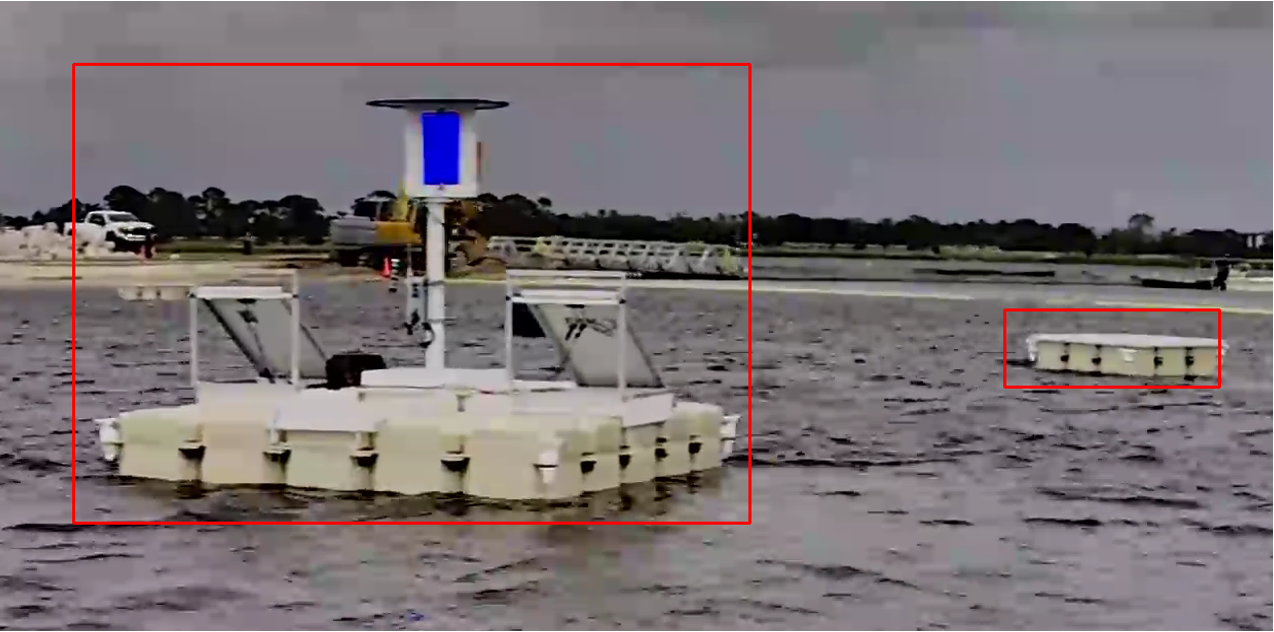
\includegraphics[width=0.5\linewidth]{Images/YOLO_ex1.png}
    \caption{Rectangular bounding boxes placed around maritime objects detected by a re-trained YOLO detection model.}
    \label{fig:YOLO_tower}
\end{figure}

The name YOLO refers to the one-shot convolutional neural network utilized to perform both detection and localization in a single pass of the network.
This architecture is what makes it fast, and for real-time object detection applications. 
Before the release of version 8 in 2023, the dual action of detection and localization required that the location and dimension of the bounding box also had to be encoded into the model.
Version 8 was the first to utilize dual-detection heads at the end of the CNN.
The first detection head identifies if and where an object is present within the image, and the second is used to determine the bounding box for the object.
This "anchor-free" architectural change not only makes localization of the detected objects more reliable, but also alleviates some of the intense transfer learning burden that was required for fine-tuning the pretrained models in earlier versions \cite{ultralytics}.

The widespread adoption of YOLOv8 and the fundamental architectural changes in this version make it the optimal choice to provide a baseline visual detection method.
% However, this mode of detection is not without its compromises, \textcolor{red}{as will be detailed in Section ____.}







% The YOLO Framework
% Describe the principle succinctly:

% YOLOv8 Architecture
% This section should flow from general framework to version-specific improvements:

% Image Resolution and Input Scaling
% Transition to operational detail and experimental consistency:

% Detection Scale and Spatial Sensitivity
% Discuss how feature maps relate to the detection limit:

% Model Constraints and Applicability
% Then note practical limitations and their relevance:

% Implications for Real-Time Fusion
% Conclude the section by connecting to your larger research goal:

% \textcolor{red}{To establish a performance baseline for real-time, vision-based object detection, this study employed the You Only Look Once (YOLO) framework, a single-stage convolutional neural network (CNN) architecture designed for end-to-end detection and classification. Unlike two-stage detectors that separately generate region proposals before classification, YOLO formulates detection as a direct regression problem, predicting bounding box coordinates and class probabilities simultaneously. This design allows all detections to occur in a single computational pass, providing the speed necessary for autonomous and embedded sensing applications. The visual detection results presented here serve as the reference modality for comparison with LiDAR-based detection methods and for evaluating computational performance in the subsequent late-fusion framework.}

% \textcolor{red}{
% The eighth-generation YOLOv8 model developed by Ultralytics was selected due to its stability, active development, and high inference efficiency on modern hardware. YOLOv8 integrates several architectural refinements that enhance accuracy and convergence speed relative to previous versions. The model employs an anchor-free detection strategy, eliminating the predefined bounding-box templates that characterized earlier YOLO iterations. Instead, YOLOv8 predicts the object center, width, and height directly, simplifying configuration and improving adaptability to objects of varying aspect ratios and scales. A decoupled detection head separates the regression and classification branches of the network, allowing independent optimization of spatial and semantic components during training. The backbone of the network uses C2f (Cross-Stage Partial Fusion) modules, which improve feature reuse and gradient flow while reducing overall computation. These modifications collectively contribute to higher accuracy and reduced latency, both of which are critical for on-board real-time inference
% The model employs modern loss functions to enhance bounding-box precision. The Complete-IoU (CIoU) loss function refines localization by incorporating geometric distance and aspect ratio penalties, while the Distribution-Focal Loss (DFL) improves boundary regression stability. Together, these losses improve the correspondence between predicted and ground-truth boxes and facilitate more consistent convergence during training. The network was implemented in PyTorch using the native Ultralytics framework, which provides integrated preprocessing, data augmentation, and export utilities. This implementation enables consistent deployment across GPU-based and embedded computing platforms without manual configuration
% }
% \textcolor{red}{
% All input frames were processed at a resolution of 640 × 640 pixels, which corresponds to YOLOv8’s default operational size and the native output of the experimental imaging system. Maintaining this native resolution avoided unnecessary interpolation and ensured a one-to-one correspondence between camera pixels and network input. YOLOv8 performs detection at three spatial scales, corresponding to feature-map strides of 8, 16, and 32 pixels relative to the input. These scales allow simultaneous sensitivity to small, medium, and large objects within a single inference pass. For a 640 × 640 input image, these feature maps have effective dimensions of 80 × 80, 40 × 40, and 20 × 20 cells, respectively. Each cell in the smallest-stride feature map represents an 8 × 8 pixel region of the input image.}
% \textcolor{red}{
% Because of this multi-scale design, the network’s minimum detectable object size is bounded by the stride of the smallest feature map. Objects must occupy multiple adjacent cells to generate distinct activations; those confined to a single cell are typically lost through downsampling or non-maximal suppression. Empirical evaluation and prior literature indicate that YOLOv8 reliably detects objects approximately 16–32 pixels in width or height—roughly 0.5–1 percent of the frame area for a 640 × 640 input. Objects smaller than this threshold generally produce low-confidence or unstable detections.}
% \textcolor{red}{
% This limitation arises from several interrelated factors. First, downsampling loss in convolutional and pooling layers reduces high-frequency detail, causing very small features to disappear from deeper network layers. Second, the receptive field of later layers covers large portions of the input image, diminishing the spatial specificity required for fine-scale detections. Third, training bias inherent to datasets such as COCO and VOC, which contain relatively large annotated objects, restricts the network’s learned sensitivity to sub-pixel features. These factors collectively define the lower bound of object detectability in standard YOLOv8 configurations.}
% \textcolor{red}{
% The 640 × 640 camera used in this study matches the network’s native input dimension, permitting direct inference without rescaling and ensuring consistent timing measurements for real-time operation. This configuration provides an accurate representation of YOLOv8’s performance under embedded deployment conditions and serves as a visual-only detection baseline against which LiDAR-based methods and fused detection results are compared in later sections. The analysis presented here therefore defines the temporal and computational characteristics of the visual detection pipeline that underpin the late-fusion approach adopted in this research.
% }

%%%%%%%%%%%%%%%%%%%%%%%%%%%%%%%%%%%%%%%%%%%%%%%%%%%%%%%%%%%%%%%%%%%%
%%%%%%%%%%%%%%%%%%%%%%%%%%%%%%%%%%%%%%%%%%%%%%%%%%%%%%%%%%%%%%%%%%%%
\section{GB-CACHE} \label{gbcache}

In parallel with vision-based detection, this research employs the LiDAR-centric method GB-CACHE to represent the class of geometry-driven clustering and segmentation algorithms.
% optimized for sparse maritime environments.
Its name is derived from the methodology it utilizes for object detection: grid-based clustering and concave hull extraction.

The segmentation approach is designed for maritime use, where point cloud data is concentrated on only a few nearby objects.
By ignoring large volumes of unoccupied space, GB-CACHE reduces memory demands and improves processing efficiency.
Its deterministic design and bounded computational complexity make it an optimal choice for real-time operation, and provide a meaningful contrast to the data-intensive, black-box nature of neural-network-based algorithms.

The algorithm begins by projecting unstructured point cloud data into a spatially organized grid defined in the global fixed frame.
Each point is associated with a primary set of $x$ and $y$ coordinates, and a tertiary $z$ coordinate to preserve vertical geometry.
Segmentation is then performed by clustering adjacent occupied cells in the $x,y$ plane according to a configurable distance parameter.
This dimensionality reduction from three to two spatial dimensions greatly reduces the computational overhead and allows the algorithm to scale linearly with size.


Each segmented object is then identified by a concave hull formed from the $x$ and $y$ vertices of a perimeter-matched polygon.
Compared to axis-aligned bounding boxes or circular boundary approximations, concave hulls more accurately reflect object geometry without overgeneralizing the object’s spatial extent.

For autonomous navigation, concave hulls offer a balance between fidelity and operational safety.
This is especially relevant in ground-based and maritime environments, where the ability to navigate between closely spaced objects depends on accurately estimating navigable pathways.
Overly conservative bounds may exaggerate the extent of objects as viewed from the vessel.
With precise object boundaries known, they can be inflated to accommodate navigational safety while maintaining an accurate representation of the object's structure.

GB-CACHE employs a \acl{MGC} to specify what class of object it has identified. 
Much like other classification methods, it utilizes a list of detected features to distinguish one class from another.
Each of the ten features it observes is provided with a brief description in Table \ref{tab:gbcache_features}.
The magnitude of an object's observed individual features may change based on distance to the object or viewing angle, but their relative values still provide valuable information.

\begin{table}[htbp]
\centering
\begin{tabular}{lll}
\hline
\multicolumn{3}{c}{GB-CACHE: Object Classification Features}\\
\hline
\hline
\textbf{No.} & \textbf{Feature Type} & \textbf{Description} \\ 
\hline
1 & Intensity (Max) & Peak LiDAR return intensity \\
2 & Intensity (Min) & Lowest LiDAR return intensity \\
3 & Intensity (Avg) & Mean LiDAR return intensity \\
4 & Intensity (Std. Deviation) & Variation in return intensity \\
5 & Height (Max) & Vertical extent of the object \\
6 & Filled Cell Count & Number of occupied grid cells \\
7 & Polygon Perimeter & Length of 2D concave hull boundary \\
8 & Polygon Area & Area of enclosed 2D concave hull \\
9 & Major Axis Length & Longer principal axis of object polygon \\
10 & Minor Axis Length & Shorter principal axis of object polygon \\
\hline
\end{tabular}
\caption{Features used for GB-CACHE multivariate classification.}
\label{tab:gbcache_features}
\end{table}

In \ac{MGC}, the values of these features are assumed to follow Gaussian distributions within each class.
By modeling the joint distribution of all ten features at once (a multivariate Gaussian), the classifier can compute a \acl{PDF} for each object class.
This enables the classifier to assign the most probable class label to the object based on the vector of all ten features, even as the individual values may fluctuate.

% \begin{figure}
%     \centering
%     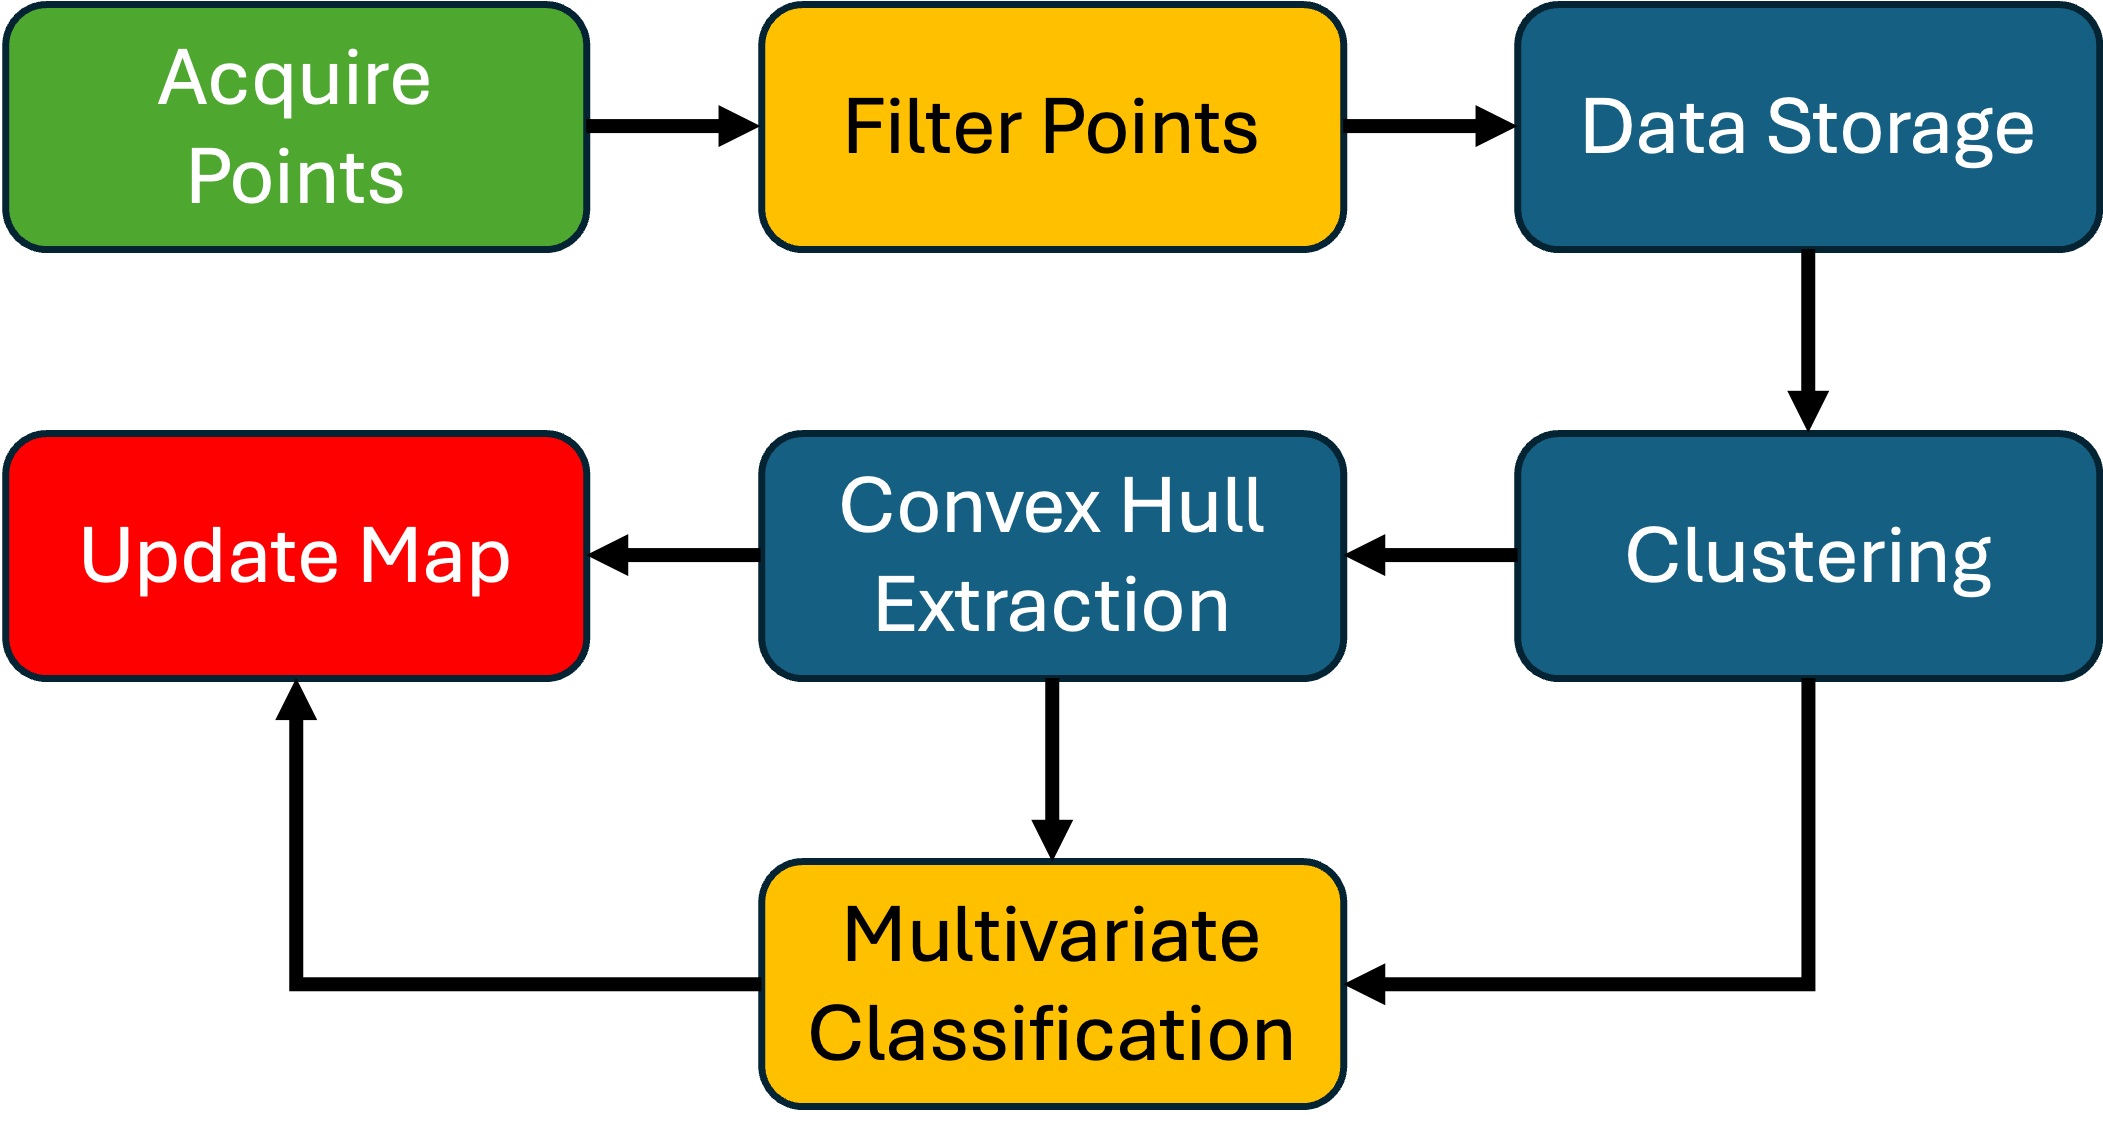
\includegraphics[width=0.95\linewidth]{Images/gbcache_flow.png}
%     \caption{Rectangular bounding boxes placed around maritime objects detected by a re-trained YOLO detection model.}
%     \label{fig:gbcache_flow}
% \end{figure}

% The YOLO Framework
% Describe the principle succinctly:

% YOLOv8 Architecture

% This section should flow from general framework to version-specific improvements:

% Image Resolution and Input Scaling
% Transition to operational detail and experimental consistency:

% Detection Scale and Spatial Sensitivity
% Discuss how feature maps relate to the detection limit:

% Model Constraints and Applicability
% Then note practical limitations and their relevance:

% Implications for Real-Time Fusion
% Conclude the section by connecting to your larger research goal:

% %%%%%%%%%%%%%%%%%%%%%%%%%%%%%%%%%%%%%%%%%%%%%%%%%%%%%%%%%%%%%%%%%%%%
% \subsection{Grid-Based Indexing} \label{sec:grid-based_indexing}

% Reliable object detection from LiDAR data is essential for safe maritime autonomy. To process large three-dimensional point clouds efficiently, this work applies the Grid-Based Clustering and Concave Hull Extraction (GB-CACHE) framework, an existing method developed for real-time segmentation of sparse LiDAR data. The approach enables rapid separation of individual objects while maintaining computational efficiency compatible with embedded vessel hardware.

% GB-CACHE operates by organizing each LiDAR scan into a structured spatial grid, allowing nearby points to be grouped without requiring full pairwise distance comparisons. This grid representation simplifies the process of identifying discrete clusters that correspond to physical objects such as buoys, vessels, or markers. By tuning grid size and connectivity thresholds, the method balances sensitivity to small targets against computational cost. In maritime environments—where LiDAR returns are sparse and concentrated on a few floating objects—the grid structure efficiently isolates relevant regions while ignoring the large volumes of empty space above and below the water surface.

% \begin{figure}
%     \centering
%     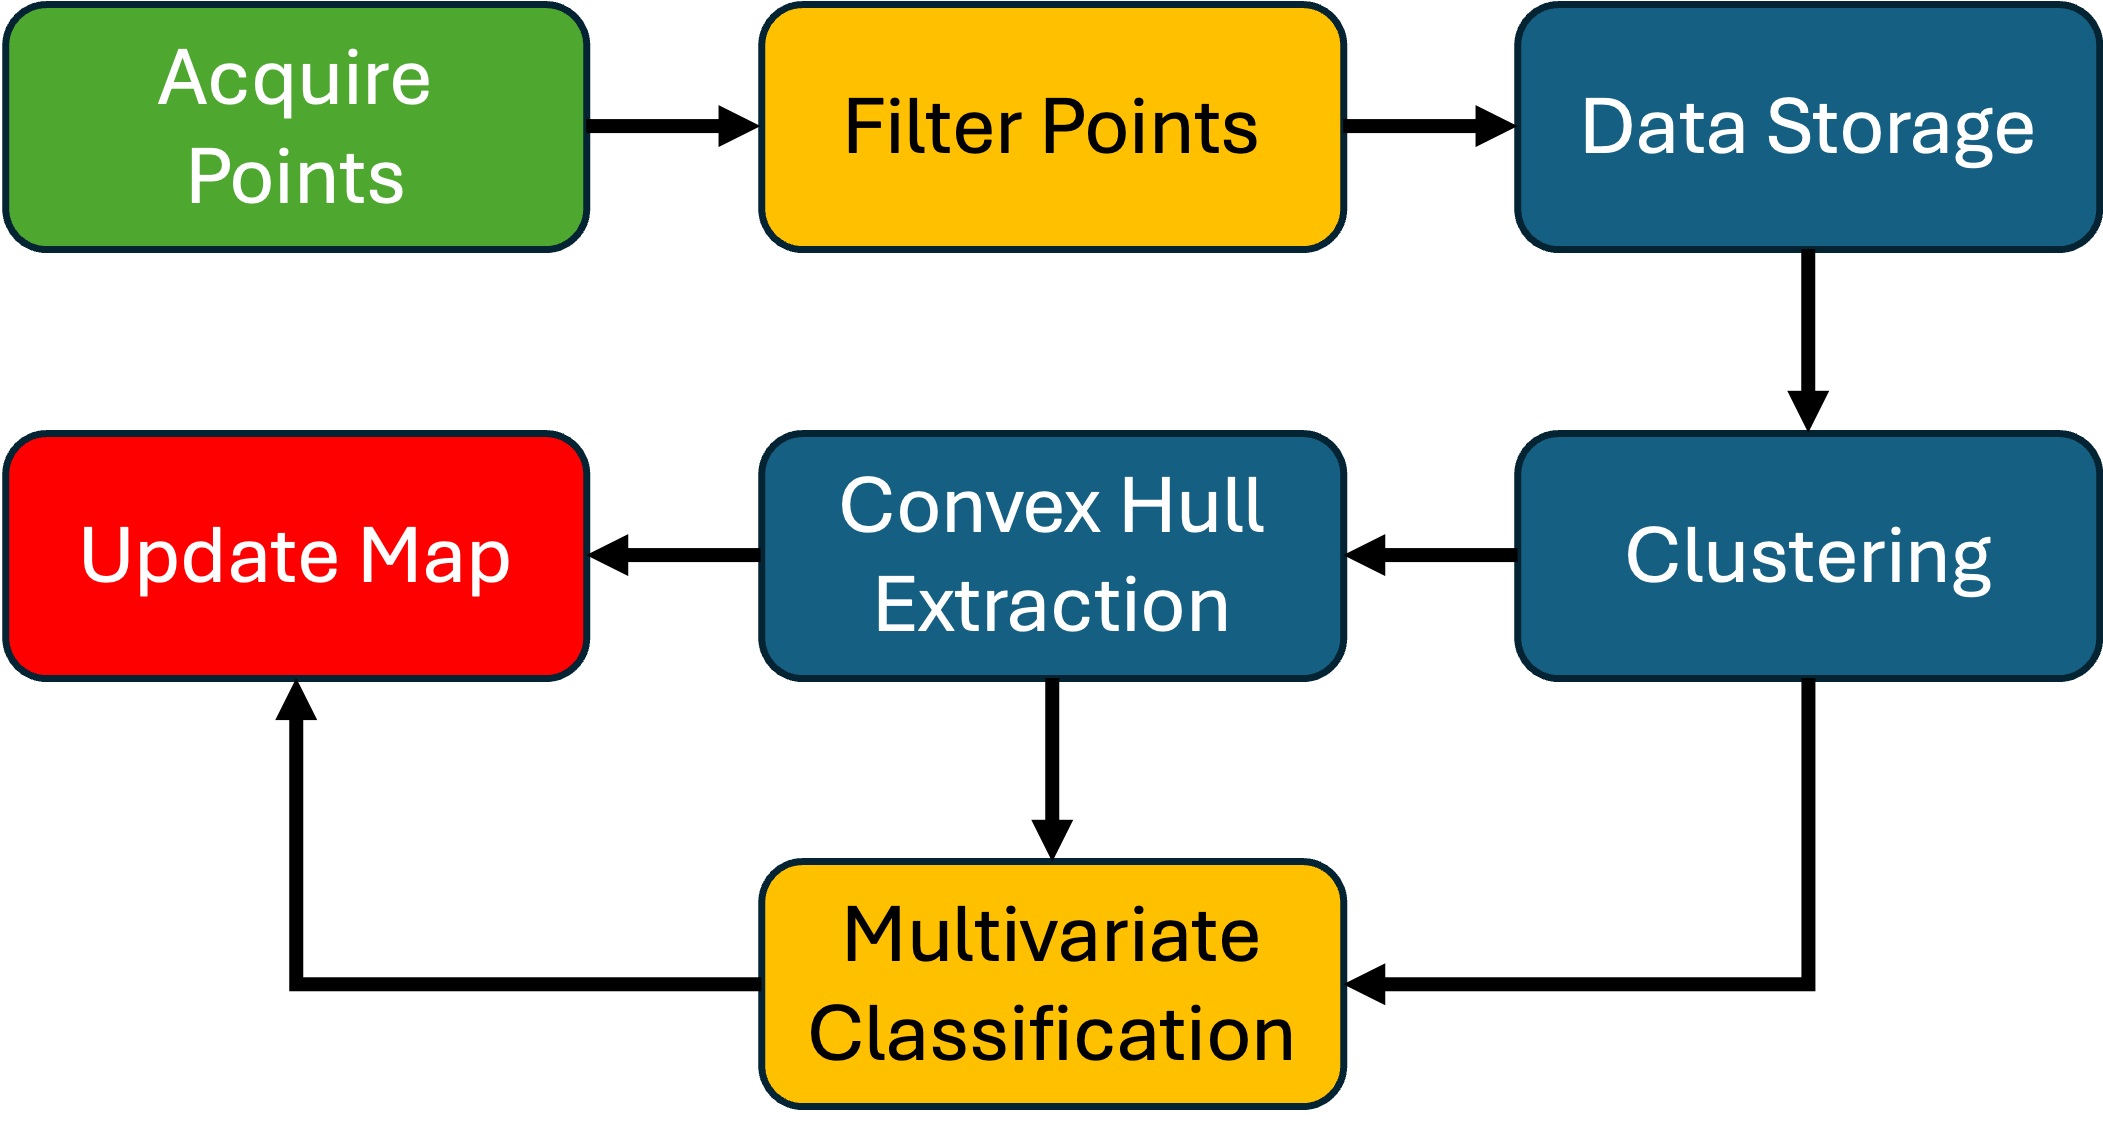
\includegraphics[width=0.5\linewidth]{Images/gbcache_flow.png}
%     \caption{Functional block diagram of the GB-CACHE workflow.}
%     \label{fig:gbcache_flow}
% \end{figure}

% Once potential objects are identified, GB-CACHE extracts geometric boundaries that define their overall shape. Each detected cluster is represented by a concave hull, which conforms closely to the true object outline rather than enclosing it with a simple convex boundary. This representation preserves important geometric details for irregular maritime targets, such as navigation buoys or vessel superstructures, while remaining compact for downstream processing. The resulting shape models form the basis for feature extraction and classification in subsequent stages of the perception pipeline.

% The algorithm’s design emphasizes computational efficiency and predictable timing. Grid-based indexing ensures that processing time scales linearly with the number of points in a scan, allowing consistent real-time performance. Each LiDAR frame is processed independently—populating the grid, segmenting occupied regions, and generating hulls—without maintaining historical state or iterative refinement. This stateless design simplifies implementation and guarantees bounded latency, which is critical for collision-avoidance and control tasks.

% GB-CACHE’s lightweight memory requirements further support real-time operation. Because memory usage scales with grid dimensions rather than total point count, resource consumption remains stable across varying environmental conditions. The method thus provides a practical and computationally efficient means of segmenting maritime LiDAR data into meaningful object candidates, serving as the front-end detection stage for the overall perception system.

% The segmentation stage of \ac{GB-CACHE} produces a structured list of clustered objects, each represented by a polygonal boundary and associated point statistics.
% The multivariate Gaussian classifier (MGC) operates in parallel to this process, classifying each object in the list based on geometric and intensity-derived features computed from its segmented point cloud.
% This architecture separates detection from classification, enabling each to be optimized and evaluated independently while maintaining real-time operation.

% For each detected object, a ten-dimensional feature vector is extracted that captures both spatial geometry and surface reflectivity characteristics.
% The geometric features describe object shape and scale, while the intensity-based features provide cues related to material properties and orientation of reflective surfaces.
% These complementary measurements form a compact yet discriminative representation suitable for statistical classification.
% The selected features are summarized in Table~\ref{tab:gbcache_features}.

% \begin{table}[htbp]
% \centering
% \begin{tabular}{lll}
% \hline
% \multicolumn{3}{c}{GB-CACHE: Object Classification Features}\\
% \hline
% \hline
% \textbf{No.} & \textbf{Feature Type} & \textbf{Description} \\ 
% \hline
% 1 & Maximum Intensity & Peak LiDAR return intensity \\
% 2 & Minimum Intensity & Lowest LiDAR return intensity \\
% 3 & Average Intensity & Mean LiDAR return intensity \\
% 4 & Intensity Standard Deviation & Variation in return intensity \\
% 5 & Maximum Height & Vertical extent of the object \\
% 6 & Filled Cell Count & Number of occupied grid cells \\
% 7 & Polygon Perimeter & Boundary length of concave hull \\
% 8 & Polygon Area & Enclosed area of concave hull \\
% 9 & 2D Minor Axis Length & Shorter principal axis of object shape \\
% 10 & 2D Major Axis Length & Longer principal axis of object shape \\
% \hline
% \end{tabular}
% \caption{Features used for GB-CACHE multivariate classification.}
% \label{tab:gbcache_features}
% \end{table}

% The MGC models the joint probability distribution of these features for each object class under the assumption of Gaussian statistics.
% Each class is represented by its mean vector and covariance matrix, estimated from labeled training data.
% During inference, the classifier computes the likelihood of an observed feature vector under each class model and assigns the class with the highest posterior probability.
% This probabilistic formulation captures correlations among features and yields confidence estimates that can be used downstream in fusion or decision logic.

% Feature-based classification offers several advantages for real-time maritime perception.
% It requires minimal training data, provides interpretability of the decision process, and imposes negligible computational overhead.
% Unlike deep-learning models that operate directly on raw point clouds, the MGC approach allows rapid retraining or adaptation to new object categories without altering the underlying clustering framework.
% This modularity supports continuous improvement and integration within the real-time perception pipeline illustrated in Figure~\ref{fig:gbcache_flow}.

% \begin{figure}[htbp]
%     \centering
%     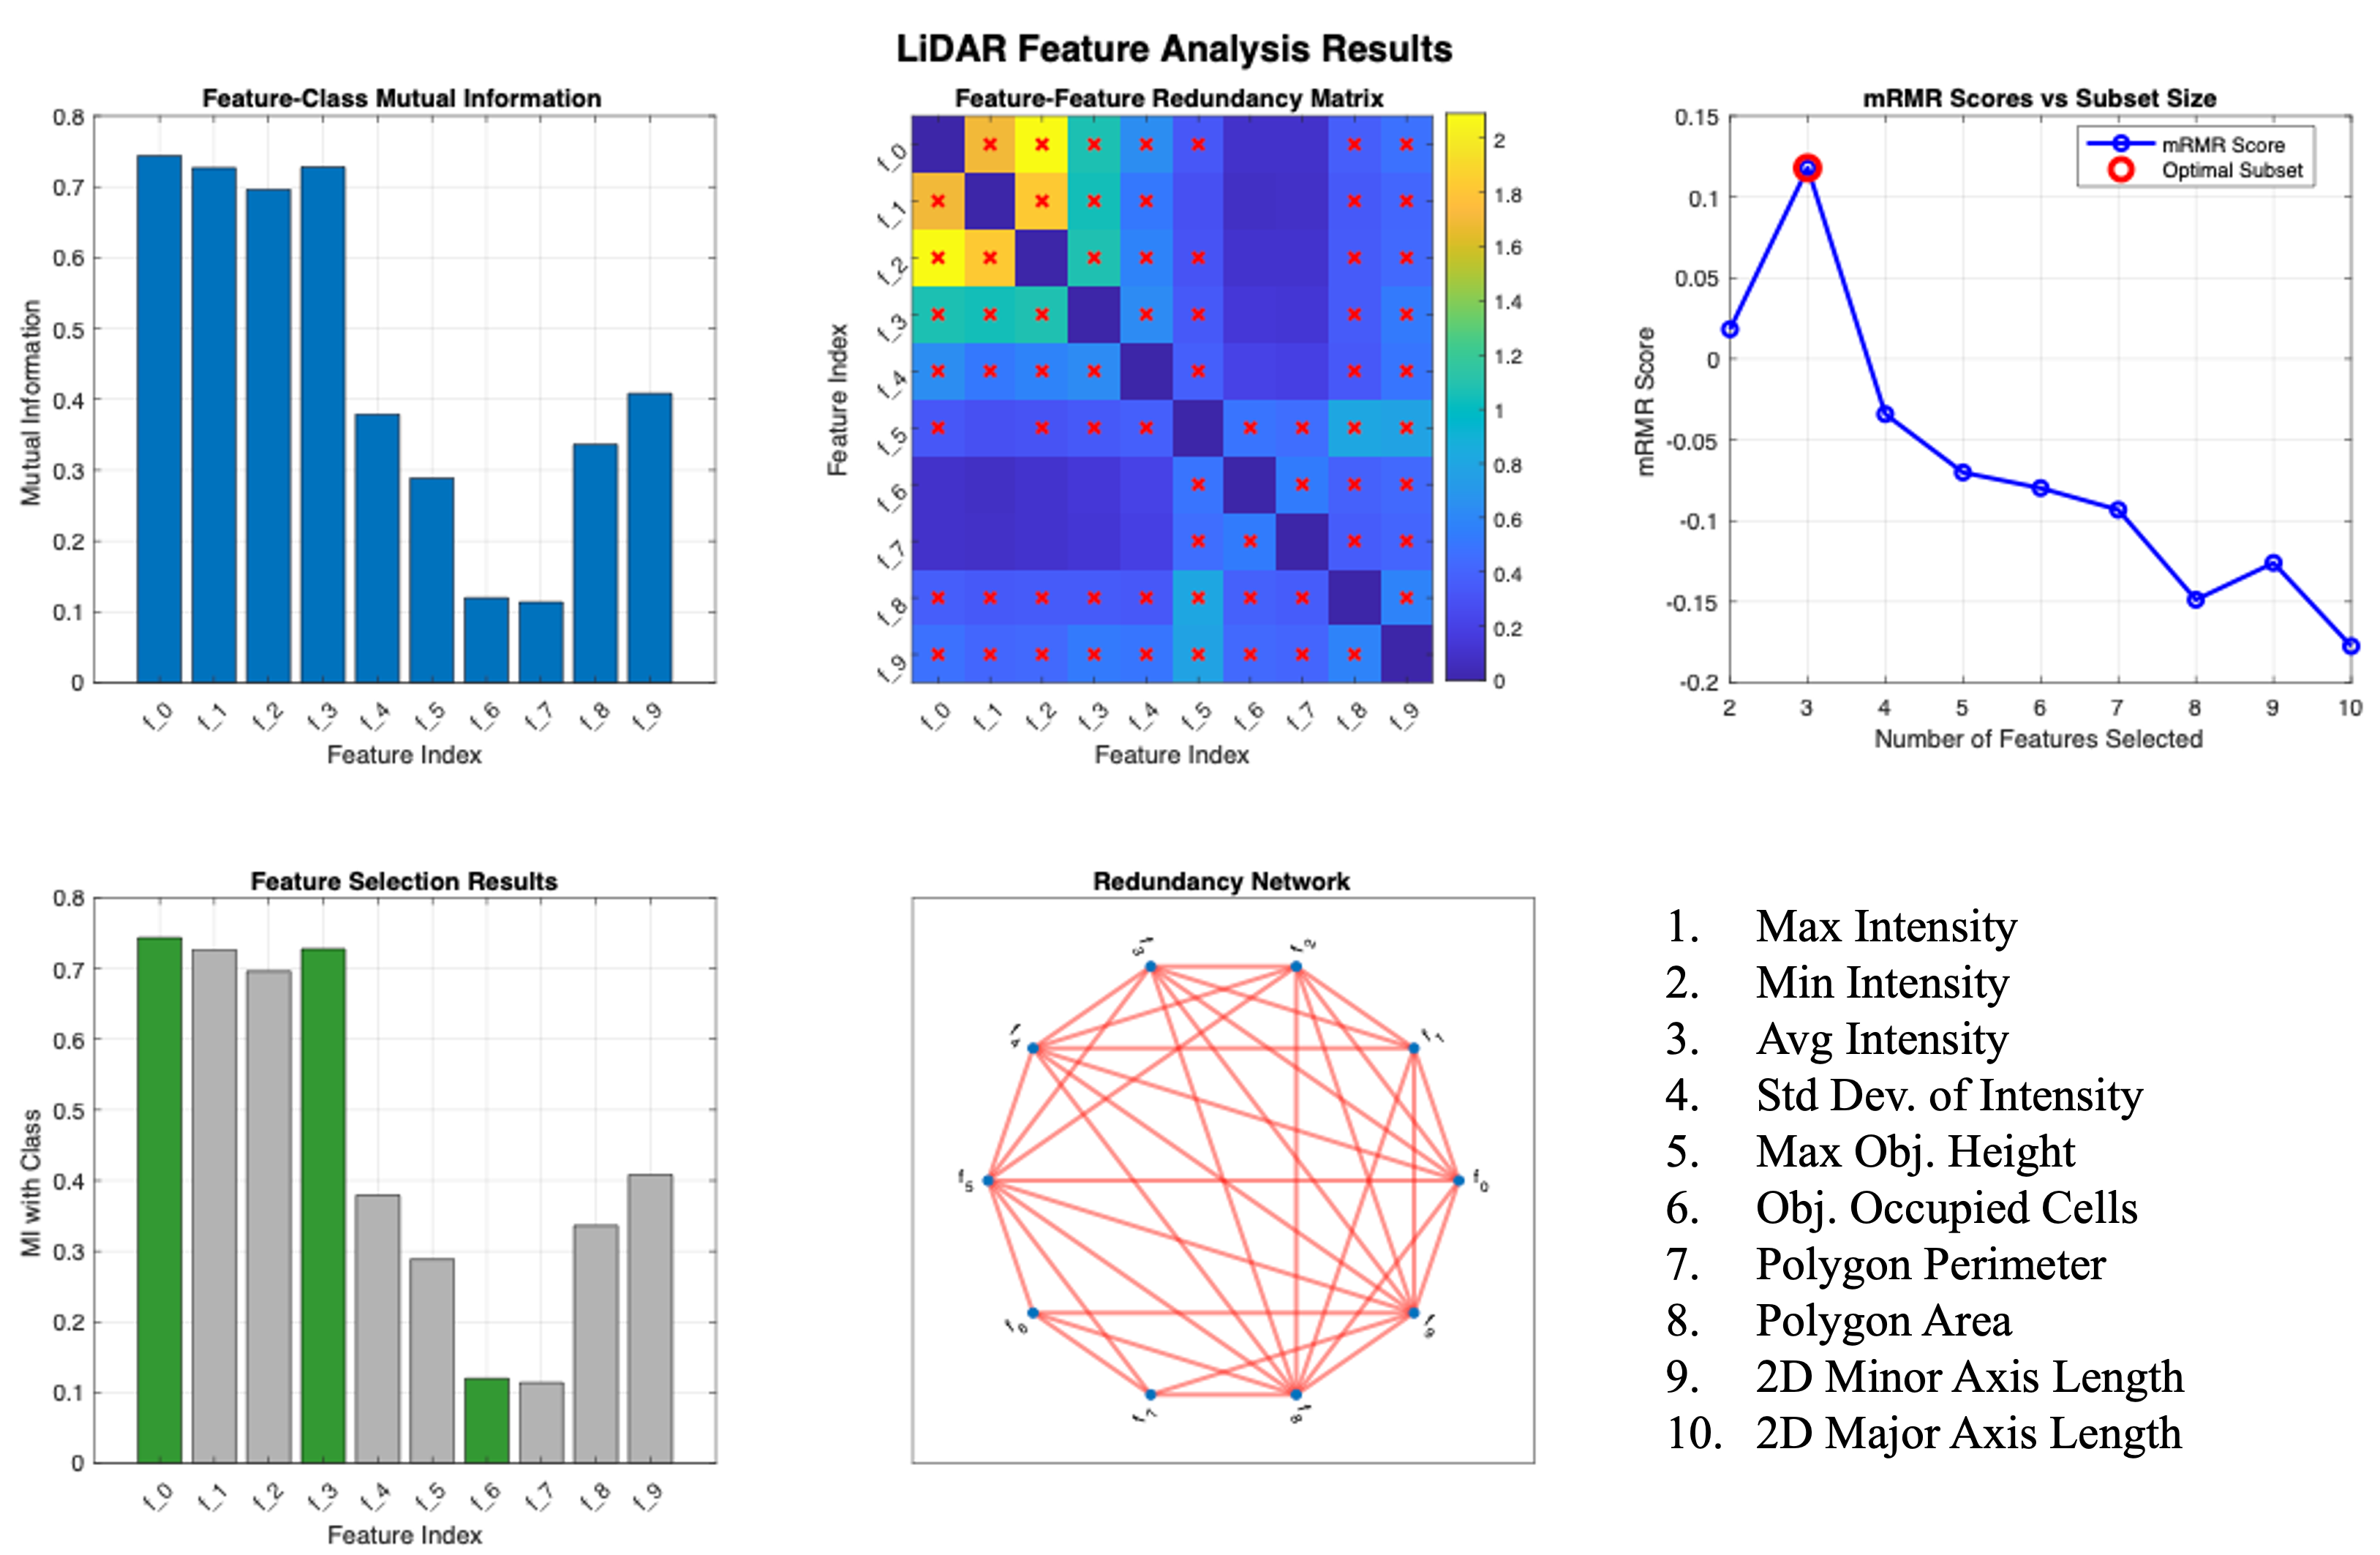
\includegraphics[width=0.95\linewidth]{Images/info_theory_chart_1.png}
%     \caption{Caption}
%     \label{fig:infoTheory_chartsA}
% \end{figure}

% \begin{figure}[htbp]
%     \centering
%     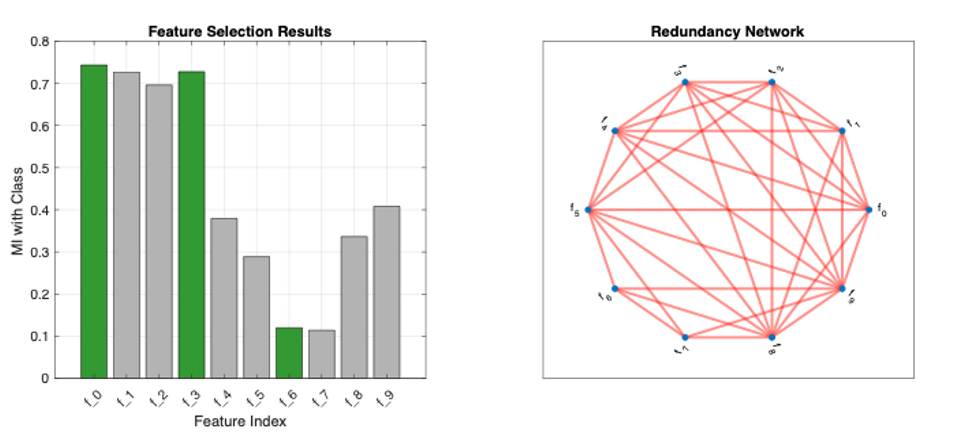
\includegraphics[width=0.8\linewidth]{Images/info_theory_chart_2.png}
%     \caption{Caption}
%     \label{fig:infoTheory_charts}
% \end{figure}



%%%%%%%%%%%%%%%%%%%%%%%%%%%%%%%%%%%%%%%%%%%%%%%%%%%%%%%%%%%%%%%%%%%%
%%%%%%%%%%%%%%%%%%%%%%%%%%%%%%%%%%%%%%%%%%%%%%%%%%%%%%%%%%%%%%%%%%%%
\section{Late Fusion} \label{late_fusion}

% \subsection{Intro}
% Introduce fusion and late fusion

% \subsection{late fusion method}
% fuse bounding boxes from YOLO with projected object bounds from GB-CACHE

% Kalman filter type reliability factor from each to produce more accurate bounds

% \paragraph{Limitations}
% corrections to GB-CACHE perimeter vertices.

% Limitations of YOLO resolution


%%%%%%%%%%%%%%%%%%%%%%%%%%%%%%%%%%%%%%%%%%%%%%%%%%%%%%%%%%%%%%%%%%%%
%%%%%%%%%%%%%%%%%%%%%%%%%%%%%%%%%%%%%%%%%%%%%%%%%%%%%%%%%%%%%%%%%%%%
\section{Model Performance} \label{performance}


%%%%%%%%%%%%%%%%%%%%%%%%%%%%%%%%%%%%%%%%%%%%%%%%%%%%%%%%%%%%%%%%%%%%
%\subsection{Yolo Performance} \label{yolo_performance}

%%%%%%%%%%%%%%%%%%%%%%%%%%%%%%%%%%%%%%%%%%%%%%%%%%%%%%%%%%%%%%%%%%%%
% \subsection{Transfer Learning and Model Fine-Tuning}
% \label{sec:yolo_finetuning}
% For this research, YOLOv8 was trained on a custom maritime dataset derived from sensor recordings collected aboard the Minion platform.
% The dataset includes labeled examples of navigation markers, buoys, vessels, and other relevant maritime objects captured under diverse lighting conditions, sea states, and viewing angles.
% Transfer learning was employed by initializing the network with weights pre-trained on a general-purpose dataset, then fine-tuning on the maritime-specific data to adapt the model to the target domain.

% Inference was conducted using the YOLOv8m variant, selected to balance detection accuracy with real-time performance on the GPU-equipped computing platform installed on Minion.
% Post-processing applies non-maximum suppression to eliminate redundant detections, retaining only the highest-confidence predictions for each detected object.
% Pre-trained YOLOv8 weights were fine-tuned on a domain-specific dataset collected from the Minion \ac{ASV} platform.  
% Transfer learning accelerates convergence and reduces the need for large labeled datasets by adapting weights from a general-purpose model (e.g., COCO) to the maritime environment.

% Fine-tuning was performed using the Ultralytics YOLOv8 framework \cite{ultralytics}, with a combination of data augmentation techniques (random flips, exposure shifts, and rotations) to increase robustness under variable lighting and sea-state conditions.
% Hyperparameters such as learning rate, batch size, and number of epochs were optimized empirically to prevent overfitting while ensuring consistent convergence.

% % \begin{figure}[htbp]
% %     \centering
% %     \includegraphics[width=0.85\linewidth]{Images/yolo_training_curve.png}
% %     \caption{Example YOLOv8 training convergence showing loss and mean Average Precision (mAP) trends over epochs.}
% %     \label{fig:yolo_training_curve}
% % \end{figure}


% To assess the tradeoff between accuracy and inference speed, three YOLOv8 variants—\textit{nano/xs}, \textit{small}, and \textit{medium}—were evaluated.
% Each model differs in backbone depth and channel width, providing progressively higher accuracy at the cost of computational complexity.
% % Table~\ref{tab:yolo_variants} summarizes model specifications and benchmark performance.

% % \begin{table}[htbp]
% % \centering
% % \caption{YOLOv8 model comparison for visual detection tasks.}
% % \begin{tabularx}{0.9\textwidth}{l c c c c}
% % \toprule
% % \textbf{Model} & \textbf{Params (M)} & \textbf{Input Size (px)} & \textbf{FPS (RTX 3090)} & \textbf{mAP@50} \\
% % \midrule
% % YOLOv8-xs & 3.2 & 640 & 110 & 0.79 \\
% % YOLOv8-s & 11.2 & 640 & 85 & 0.84 \\
% % YOLOv8-m & 25.9 & 640 & 63 & 0.87 \\
% % \bottomrule
% % \end{tabularx}
% % \label{tab:yolo_variants}
% % \end{table}

% Inference timing was recorded using per-process timers to isolate image capture, pre-processing, neural inference, and post-processing durations.
% This timing-based comparison allows fair assessment against non-GPU LiDAR pipelines in later sections.

% %%%%%%%%%%%%%%%%%%%%%%%%%%%%%%%%%%%%%%%%%%%%%%%%%%%%%%%%%%%%%%%%%%%%
% \subsection{Retraining Results and Performance Evaluation}
% \label{sec:yolo_results}

% The fine-tuned YOLOv8-s model achieved the best balance of accuracy and speed for maritime operations.
% Model evaluation was performed using a holdout dataset collected under variable illumination and sea states.
% Performance metrics include mean Average Precision (mAP@50), precision-recall curves, and confusion matrices for key object classes such as vessels, buoys, and docks.

% \begin{figure}[htbp]
%     \centering
%     \includegraphics[width=0.8\linewidth]{Images/yolo_confusion_matrix.png}
%     \caption{Confusion matrix for YOLOv8-s model evaluated on the test dataset.}
%     \label{fig:yolo_confusion_matrix}
% \end{figure}

% \begin{figure}[htbp]
%     \centering
%     \includegraphics[width=0.8\linewidth]{Images/yolo_pr_curve.png}
%     \caption{Precision–recall curve for primary object classes.}
%     \label{fig:yolo_pr_curve}
% \end{figure}

% Results indicate consistent detection performance across lighting conditions with minimal false positives on horizon clutter.
% Retraining improved small-object detection by approximately X\% compared to baseline COCO-trained weights, confirming the benefit of domain adaptation for maritime imagery.

% %%%%%%%%%%%%%%%%%%%%%%%%%%%%%%%%%%%%%%%%%%%%%%%%%%%%%%%%%%%%%%%%%%%%
% \subsection{Discussion and Relevance to Sensor Fusion}
% \label{sec:yolo_discussion}

% The fine-tuned YOLOv8 network serves as the visual baseline for comparison with LiDAR-based object detection methods presented in Section~\ref{gbcache}.
% By isolating timing metrics for each processing stage, the performance comparison remains hardware-agnostic.
% This approach emphasizes algorithmic latency, rather than total frame rate, as the primary metric for evaluating real-time feasibility in multi-sensor fusion.

%%%%%%%%%%%%%%%%%%%%%%%%%%%%%%%%%%%%%%%%%%%%%%%%%%%%%%%%%%%%%%%%%%%%
\subsection{Computational Efficiency} \label{sec:gbcache_efficiency}

The algorithmic design of \ac{GB-CACHE} prioritizes computational efficiency to enable real-time processing on autonomous surface vessel hardware with limited computing resources.
Grid-based spatial indexing reduces clustering complexity from quadratic to linear in the number of points, while the regular grid structure enables vectorized operations and cache-efficient memory access patterns.
These optimizations prove essential for maintaining detection frame rates sufficient for autonomous navigation, where delayed perception degrades collision avoidance performance.

The GB-CACHE processing pipeline operates incrementally on each \ac{LiDAR} scan, maintaining no temporal history and requiring no iterative refinement.
This design guarantees bounded worst-case execution time, critical properties for safety-critical autonomous systems.
Each scan undergoes independent processing: grid population, clustering, hull extraction, and feature calculation, producing object detections with consistent latency.

Memory requirements scale with grid dimensions rather than point count, providing predictable resource consumption independent of scene complexity.
The grid representation compresses sparse maritime point clouds into compact occupancy structures, reducing memory bandwidth requirements compared to maintaining full point coordinates.
This compression proves particularly advantageous for maritime environments where objects occupy a small fraction of the sensor's field of view.

\begin{figure}
    \centering
    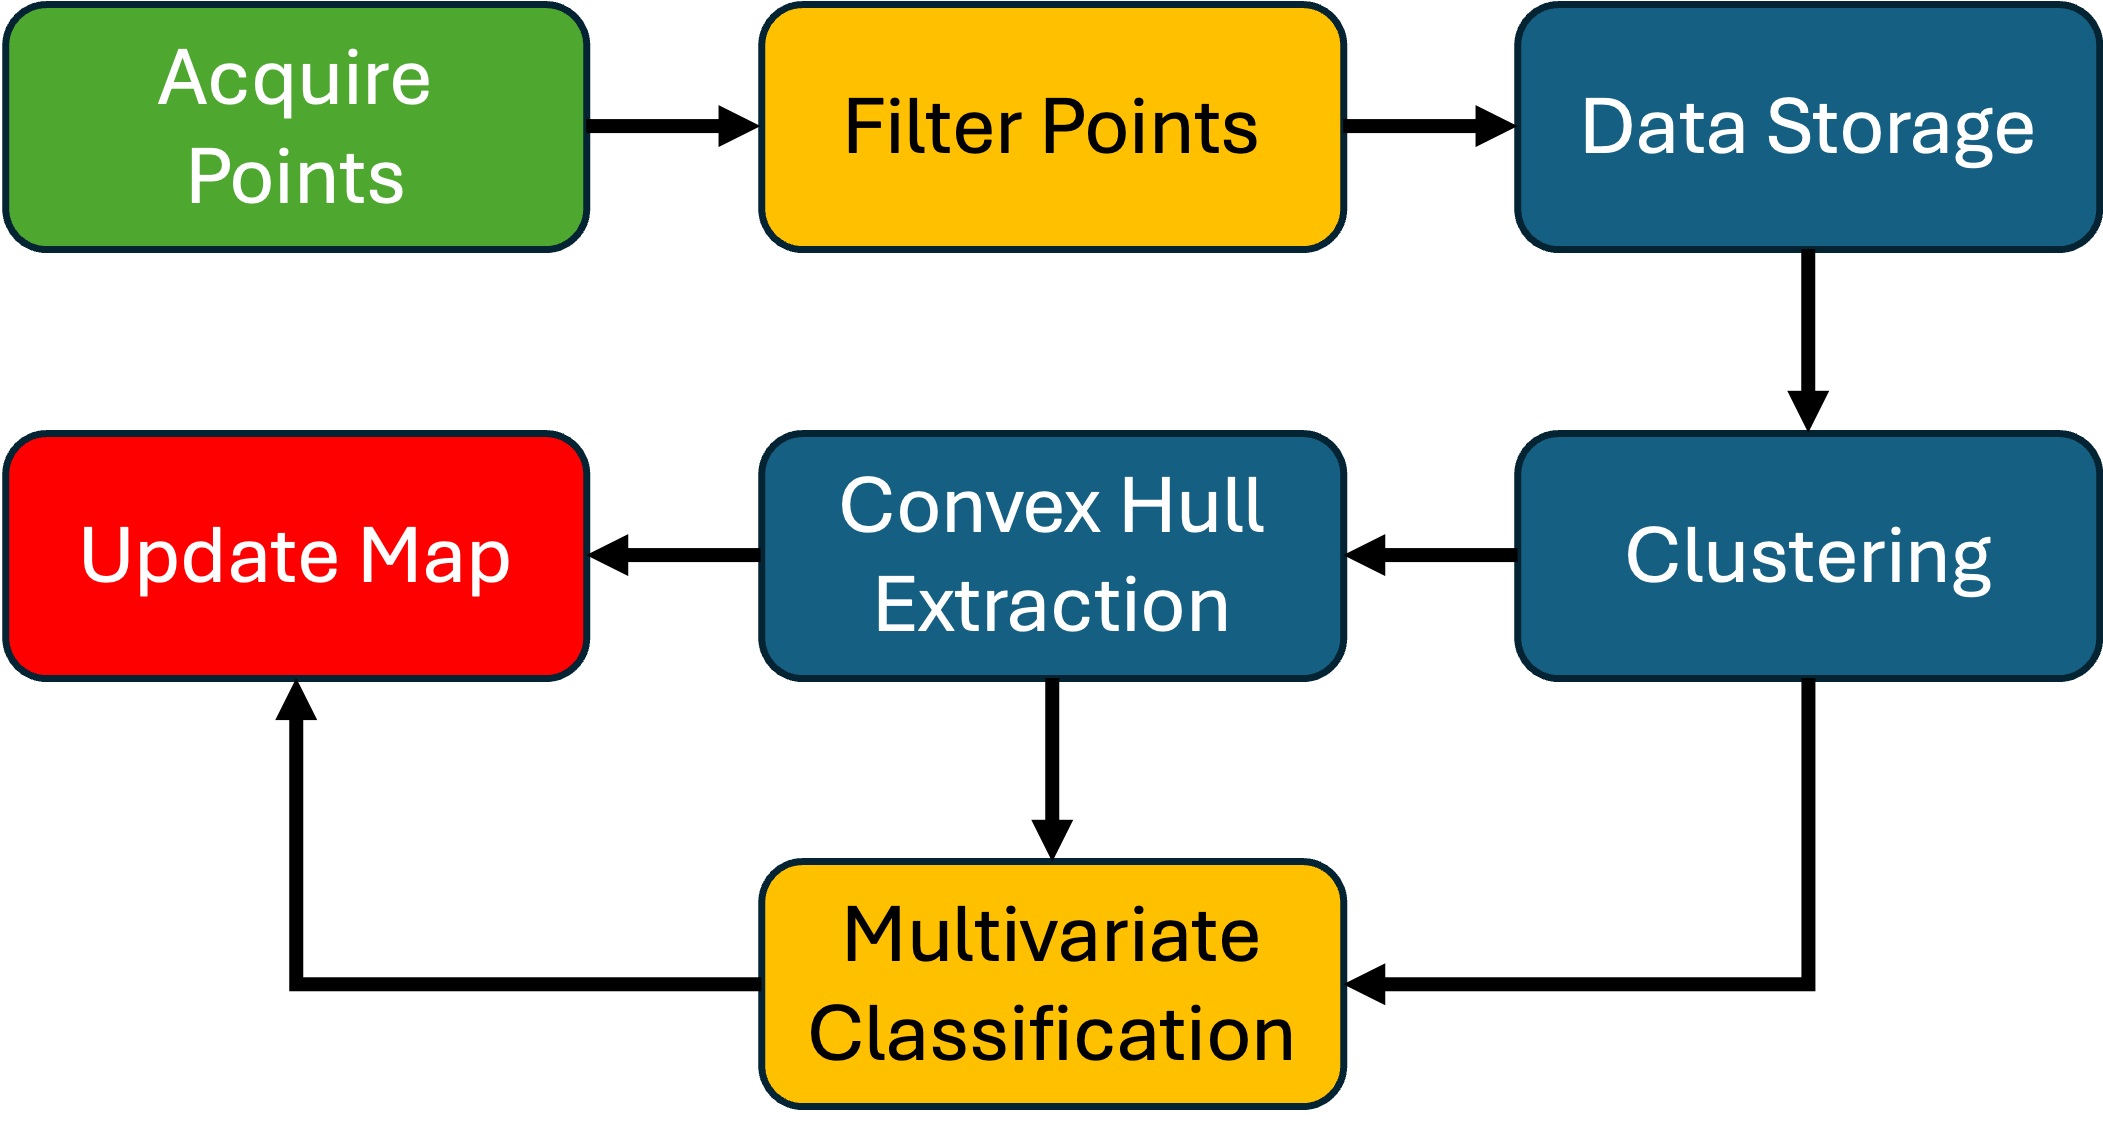
\includegraphics[width=0.95\linewidth]{Images/gbcache_flow.png}
    \caption{Caption}
    \label{fig:gbcache_flow}
\end{figure}

Performance analysis of the \ac{GB-CACHE} implementation on the Minion platform demonstrates exceptional computational efficiency compatible with real-time autonomous navigation requirements.
The spatial filtering and point addition operations execute with sub-millisecond latency, consuming negligible fractions of available processing time at sensor frame rates.
The map update operation, while more computationally intensive, exhibits strong linear correlation with object geometric complexity, specifically polygon perimeter and surface area.
This predictable scaling behavior enables reliable worst-case execution time estimation for safety-critical autonomous systems.
Hardware resource utilization remains minimal during typical operation, with both processor and memory consumption well below capacity thresholds, providing substantial computational headroom for concurrent navigation and control processes.
Detailed performance characterization across diverse maritime object encounters validates the algorithm's suitability for sustained real-time operation under operational constraints.

\begin{figure}[htbp]
\centering
\makebox[\textwidth][c]{
    \begin{subfigure}[t]{0.44\textwidth}
        \centering
        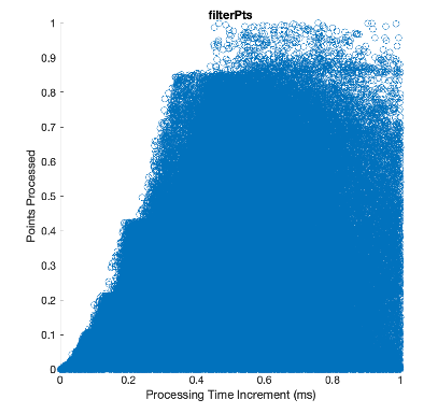
\includegraphics[width=\textwidth]{Images/gbcache/filter_points_scatter.png}
        \caption{Scatter plot of duration of \texttt{filter\_points} against number of LiDAR points}
        \label{fig:gbcache_filter_points_scatter}
    \end{subfigure}
    \hspace{2em} % horizontal spacing between them
    \begin{subfigure}[t]{0.44\textwidth}
        \centering
        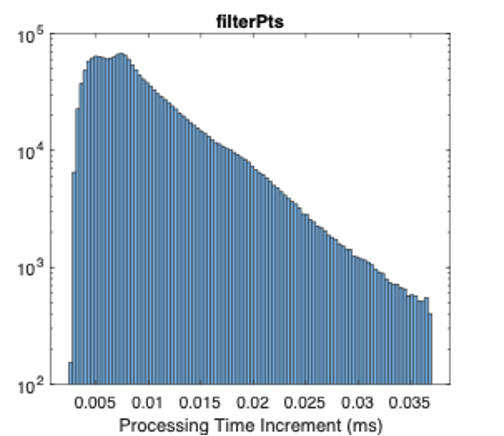
\includegraphics[width=\textwidth]{Images/gbcache/filter_points_hist.png}
        \caption{Histogram of duration of \texttt{filter\_points} against number of LiDAR points}
        \label{fig:gbcache_filter_points_hist}
    \end{subfigure}
}
\caption{Scatter (a) and histogram (b) plots of \texttt{filter\_points} process plotted against number of LiDAR points}
\label{fig:gbcache_filter_points}
\end{figure}

\begin{figure}[htbp]
\centering
\makebox[\textwidth][c]{
    \begin{subfigure}[t]{0.44\textwidth}
        \centering
        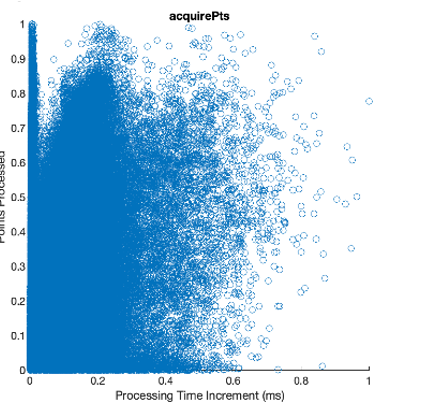
\includegraphics[width=\textwidth]{Images/gbcache/Add_points_scatter.png}
        \caption{Scatter plot of duration of \texttt{add\_points} against number of LiDAR points}
        \label{fig:gbcache_add_points_scatter}
    \end{subfigure}
    \hspace{2em} % horizontal spacing between them
    \begin{subfigure}[t]{0.44\textwidth}
        \centering
        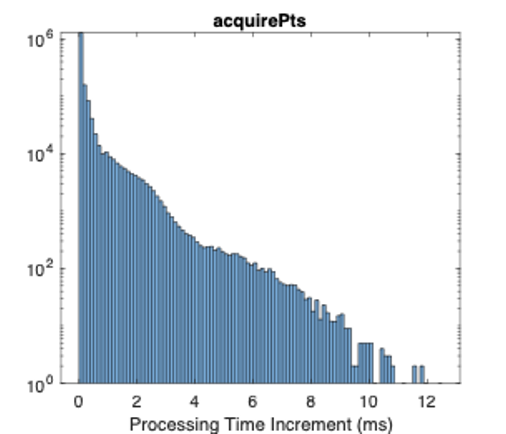
\includegraphics[width=\textwidth]{Images/gbcache/Add_points_hist.png}
        \caption{Histogram of duration of \texttt{add\_points} against number of LiDAR points}
        \label{fig:gbcache_add_points_hist}
    \end{subfigure}
}
\caption{Scatter (a) and histogram (b) plots of \texttt{add\_points} process plotted against number of LiDAR points}
\label{fig:gbcache_add_points}
\end{figure}

\begin{figure}[htbp]
    \centering
    % Subfigure (a)
    \begin{subfigure}[b]{0.44\linewidth}
        \centering
        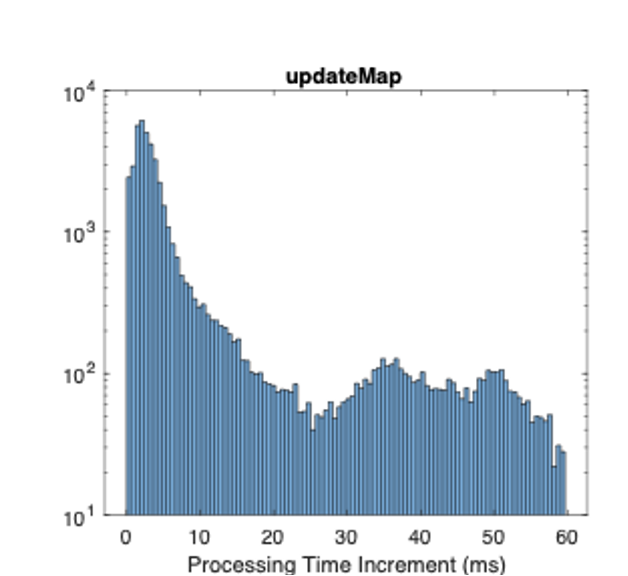
\includegraphics[width=\linewidth]{Images/gbcache/Update_Map_hist.png}
        \caption{Histogram of duration of \texttt{map\_update} against number of LiDAR points}
        \label{fig:gbcache_update_map_hist}
    \end{subfigure}
    \vspace{1em} % vertical spacing between subfigures
    % Subfigure (b)
    \begin{subfigure}[b]{0.8\linewidth}
        \centering
        \includegraphics[width=\linewidth]{Images/gbcache/Update_Map_scatter.png}
        \caption{Two scatter plot of duration of \texttt{map\_update} against average perimeter length of polygon (left), and against average area of polygon (right). The line of best-fit is shown in red for each, with associated polynomial values of: $x^2 = -0.0727, x^1 = -0.0151, x^0 = -0.0151$ (left) and $x^2 = 0.2556, x^1 = -0.00913, x^0 = -0.00913$ (right) }
        \label{fig:gbcache_update_map_scatter}
    \end{subfigure}

    \caption{Histogram (a) and scatter (b) plots of \texttt{map\_update} process plotted against number of LiDAR points}
    \label{fig:gbcache_update_map}
\end{figure}

%%%%%%%%%%%%%%%%%%%%%%%%%%%%%%%%%%%%%%%%%%%%%%%%%%%%%%%%%%%%%%%%%%%%
\subsection{Mutual Information Analysis of Features} \label{sec:gbcache_MI_features}

While the ten-feature set provides comprehensive object characterization, not all features contribute equally to classification performance, and some features exhibit redundancy through correlation.
I applied information-theoretic feature selection methodology to identify the optimal feature subset that maximizes classification accuracy while minimizing computational burden and correlation-induced instability.

The minimum Redundancy Maximum Relevance (mRMR) criterion provides a principled framework for feature selection by simultaneously considering two competing objectives: maximizing the mutual information between selected features and class labels (relevance) while minimizing the mutual information among selected features themselves (redundancy).
Mutual information quantifies the reduction in uncertainty about one variable given knowledge of another, providing a model-agnostic measure of statistical dependence applicable to both linear and nonlinear relationships.

Analysis of feature-class mutual information reveals varying discriminative power across the ten features, with intensity-based and geometric features exhibiting complementary strengths for different object classes.
Pairwise feature redundancy analysis identifies multiple correlated feature pairs that provide overlapping information, suggesting opportunities for dimensionality reduction without classification performance degradation.
The mRMR optimization procedure balances these considerations, progressively selecting features that contribute novel discriminative information while avoiding redundant measurements.

Information-theoretic analysis identified an optimal feature subset substantially smaller than the complete ten-feature set, demonstrating that effective maritime object classification can be achieved with reduced feature dimensionality.
This finding has practical implications for computational efficiency, as feature extraction and Gaussian density evaluation scale with feature dimensionality.
The reduced feature set maintains robust classification performance while decreasing processing requirements and reducing the risk of overfitting when training data is limited.

The classifier requires training data comprising labeled examples of each object class with corresponding feature vectors.
Training involves computing maximum likelihood estimates of Gaussian distribution parameters for each class, specifically the mean vector and covariance matrix that characterize the feature space distribution.
These parameters fully specify the class models, enabling rapid inference through simple multivariate Gaussian density evaluation without iterative optimization or complex neural network forward passes.

Classification performance depends critically on the separability of object classes in the chosen feature space and the validity of the Gaussian distribution assumption.
When classes exhibit significant overlap in feature space or when feature distributions deviate substantially from Gaussian, classification accuracy degrades.
However, for maritime objects with distinct geometric profiles and size ranges, the feature-based Gaussian approach provides robust classification with minimal training requirements.

\begin{figure}
    \centering
    \includegraphics[width=0.95\linewidth]{Images/MI_analysis.png}
    \caption{Caption}
    \label{fig:MI_analysis}
\end{figure}

\begin{figure}
    \centering
    \includegraphics[width=0.95\linewidth]{Images/MI_pairwise.png}
    \caption{Caption}
    \label{fig:MI_pairwise}
\end{figure}

%%%%%%%%%%%%%%%%%%%%%%%%%%%%%%%%%%%%%%%%%%%%%%%%%%%%%%%%%%%%%%%%%%%%
%%%%%%%%%%%%%%%%%%%%%%%%%%%%%%%%%%%%%%%%%%%%%%%%%%%%%%%%%%%%%%%%%%%%
%%%%%%%%%%%%%%%%%%%%%%%%%%%%%%%%%%%%%%%%%%%%%%%%%%%%%%%%%%%%%%%%%%%%

\chapter{Conclusions} 

% This chapter will synthesize findings from all three research objectives:
% - Summary of comparative performance results between LiDAR and vision systems
% - Calibration and synchronization framework effectiveness
% - Real-time processing capability validation
% - Implications for ASV perception system design
% - Contribution to maritime autonomous systems knowledge

\section{Research Objective Achievement Summary}
% Placeholder for objective completion summary

\section{Performance Comparison Findings}
% Placeholder for key comparative analysis conclusions

\section{Implications for ASV System Design}
% Placeholder for practical design guidance conclusions

\chapter{Recommendations and Future Work} 

\section{Recommendations} \label{recommendations}

\section{Future Work} \label{futurework}

This dual-system configuration facilitated the transition of Minion's software during the period of this research.
\ac{ROS} 1 was the operational framework for all research and data collected in this study, however, \ac{ROS} 1 has entered end-of-life for active development.
Consequently, Minion’s software architecture was gradually migrated to \ac{ROS} 2, which introduces substantial improvements in real-time performance, memory management, and inter-process communication.
In contrast to ROS 1’s reliance on a centralized message broker, ROS 2 employs a Data Distribution Service-based communication layer that reduces latency and memory overhead through zero-copy data handling and improved resource allocation.
Maintaining one system on ROS 1 while transitioning the other to ROS 2 allowed incremental software migration without interrupting field operations—laying the groundwork for future runtime performance improvements anticipated in Section~\ref{futurework}.

% This chapter will address:
% - Recommendations for ASV perception system design based on findings
% - Sensor selection guidance for maritime applications
% - Future research directions for maritime sensor fusion
% - Technology transfer opportunities to operational systems

\section{ASV Perception System Design Recommendations}
% Placeholder for design guidance recommendations

\section{Future Research Directions}
% Placeholder for future work recommendations

\section{Technology Transfer Opportunities}
% Placeholder for practical application recommendations




% \printbibliography
% \bibliographystyle{plainnat} - Most recent
\bibliographystyle{IEEEtranN} % natbib-compatible numeric IEEE style
% \bibliography{References}
\bibliography{Dissertation,extra_cite}

\backmatter

\chapter{Image Transform} \label{img_tform}

To obtain the two-dimensional pixel coordinates of the distorted image ($u, v$) in the camera frame $C$ from a three-dimensional coordinate ($X_{L}, Y_L, Z_L$) in the LiDAR frame $L$:

% 3D LiDAR point to distorted image pixel
% \paragraph{Projection from LiDAR to image.}
Let $\mathbf{R}\in \mathbb{R}^{3\times3}$, $\mathbf{t}\in \mathbb{R}^{3\times1}$, $_L\mathbf{P} = [X_L, Y_L, Z_L, 1]^T$,  and $_C\mathbf{P} = \;_{C}^{L}\mathbf{T} \; _L\mathbf{P}$, then:
\begin{equation*}
_C\mathbf{P} = [X_C, Y_C, Z_C, 1]^T \;= \; _{C}^{L}\mathbf{T} \;[X_L, Y_L, Z_L, 1]^T,
% ,\qquad
% _{C}^{L}\mathbf{T} =
% \begin{bmatrix}
% \mathbf{R}_{C}^{L} & \mathbf{t}_{C}^{L} \\
% \mathbf{0}^T & 1
% \end{bmatrix}.
% \label{eq:LiDAR_to_cam_frame}
\end{equation*}

such that:
\begin{equation*}
    _{L}^{C}\mathbf{T} =
    \begin{bmatrix}
        _{L}^{C}\mathbf{R} & _{L}^{C}\mathbf{t} \\
        \mathbf{0}^\mathrm{T} & 1
    \end{bmatrix},
\end{equation*}

We obtain the pixel coordinates ($x_n, y_n$) in the undistorted image frame by pinhole projection:
\begin{equation*}
x_n = \frac{X_C}{Z_C}, \qquad
y_n = \frac{Y_C}{Z_C}, \qquad
r^2 = x_n^2 + y_n^2 .
\label{eq:normalized_coords}
\end{equation*}

Apply the radial distortion model:
\begin{align*}
r^2 & = x_n^2 + y_n^2 .\\
x' & = x_n\!\left(1 + k_1 r^2 + k_2 r^4 + k_3 r^6\right), \\
y' & = y_n\!\left(1 + k_1 r^2 + k_2 r^4 + k_3 r^6\right).
\label{eq:radial_distortion_apply}
\end{align*}

Map ($x', y'$) to distorted pixel coordinates ($u,v$) using the intrinsic matrix $\mathbf{K}$:
\begin{equation}
\begin{bmatrix} u \\ v \\ 1 \end{bmatrix}
=
\begin{bmatrix}
f_x & s & c_x \\
0   & f_y & c_y \\
0   & 0   & 1
\end{bmatrix}
\begin{bmatrix} x' \\ y' \\ 1 \end{bmatrix},
\qquad
% \mathbf{K} =
% \begin{bmatrix}
% f_x & s & c_x \\
% 0   & f_y & c_y \\
% 0   & 0   & 1
% \end{bmatrix},
% \quad
\Rightarrow\ 
\begin{cases}
u = f_x x' + s y' + c_x,\\
v = f_y y' + c_y.
\end{cases}
\label{eq:intrinsics_to_pixels}
\end{equation}

% \chapter{test 2}

% \begin{figure}[htbp]
%        \centering
%        % TikZ Flowchart for GStreamer HDR Pipeline
% Drop-in code for Overleaf
% Requires: \usepackage{tikz}
%          \usetikzlibrary{shapes.geometric, arrows}

\tikzstyle{process} = [rectangle, minimum width=3cm, minimum height=1cm, text centered, draw=black, fill=white, text width=3cm]
\tikzstyle{timestamp} = [rectangle, minimum width=3cm, minimum height=1cm, text centered, draw=red, line width=1.5pt, fill=white, text width=3cm]
\tikzstyle{queue} = [rectangle, minimum width=2.5cm, minimum height=0.8cm, text centered, draw=blue, line width=1.2pt, fill=white, text width=2.5cm]
\tikzstyle{output} = [rectangle, minimum width=2.5cm, minimum height=1cm, text centered, draw=green!60!black, line width=1.2pt, fill=white, text width=2.5cm, rounded corners]
\tikzstyle{decision} = [diamond, minimum width=2cm, minimum height=1cm, text centered, draw=black, fill=white, aspect=2]
\tikzstyle{arrow} = [thick,->,>=stealth]

\begin{tikzpicture}[node distance=2cm]

% Source
\node (source) [process] {\textbf{v4l2src / videotestsrc} \\ YUY2, 2880x1860@60fps \\ do-timestamp=TRUE};

% Timestamp Probe 1
\node (ts1) [timestamp, below of=source] {\textbf{TIMESTAMP PROBE \#1} \\ timestamp\_probe\_cb \\ Adds CustomTimestampMeta \\ gettimeofday() $\rightarrow$ ms};

% Tee
\node (tee) [decision, below of=ts1, yshift=-0.5cm] {\textbf{TEE (Splits 3x)}};

% Stream Branch (left)
\node (qs) [queue, below of=tee, xshift=-8cm, yshift=-1.5cm] {\textbf{queue\_stream} \\ {[BUFFER QUEUE]}};
\node (vr) [process, below of=qs] {\textbf{videorate} \\ 60fps $\rightarrow$ 5fps};
\node (nvc1) [process, below of=vr] {\textbf{nvvidconv} \\ YUY2 $\rightarrow$ I420 \\ NVMM memory};
\node (h264e) [process, below of=nvc1] {\textbf{nvv4l2h264enc} \\ H264 encode \\ bitrate=calc \\ insert-sps-pps=true};
\node (sei) [timestamp, below of=h264e] {\textbf{TIMESTAMP PROBE \#2} \\ sei\_insert\_probe\_cb \\ Reads CustomTimestampMeta \\ Inserts SEI NAL unit};
\node (h264p) [process, below of=sei] {\textbf{h264parse} \\ Parse H264 stream};
\node (rtp) [process, below of=h264p] {\textbf{rtph264pay} \\ RTP payload \\ config-interval=1 \\ mtu=1400};
\node (udp) [output, below of=rtp] {\textbf{udpsink} \\ host=201.7.90.18 \\ port=5603 \\ sync=false};

% Record Branch (middle)
\node (qr) [queue, below of=tee, yshift=-1.5cm] {\textbf{queue\_record} \\ {[BUFFER QUEUE]}};
\node (nvc2) [process, below of=qr] {\textbf{nvvidconv} \\ YUY2 $\rightarrow$ I420 \\ NVMM memory};
\node (h265e) [process, below of=nvc2] {\textbf{nvv4l2h265enc} \\ H265 encode \\ bitrate=80Mbps \\ iframeinterval=1};
\node (h265p) [process, below of=h265e] {\textbf{h265parse} \\ Parse H265 \\ byte-stream};
\node (split) [output, below of=h265p, yshift=-1cm] {\textbf{splitmuxsink} \\ muxer=qtmux \\ Split @120s \\ /mnt/logs/hdr-0/ \\ hdr-0-\{time\}-\{n\}.mp4};

% CSV Branch (right)
\node (qc) [queue, below of=tee, xshift=8cm, yshift=-1.5cm] {\textbf{queue} \\ {[BUFFER QUEUE]}};
\node (id) [process, below of=qc] {\textbf{identity} \\ csv\_identity \\ signal-handoffs=true};
\node (csv) [timestamp, below of=id] {\textbf{TIMESTAMP LOGGER} \\ csv\_handoff\_handler \\ Reads CustomTimestampMeta \\ Logs: frame\#,timestamp};
\node (csvf) [output, below of=csv, xshift=-2.5cm, yshift=-0.5cm] {\textbf{CSV Files} \\ /mnt/logs/hdr-0/ \\ hdr-0-\{time\}-\{n\}.csv \\ Split @120s};
\node (fake) [output, below of=csv, xshift=2.5cm, yshift=-0.5cm] {\textbf{fakesink} \\ discard};

% Arrows
\draw [arrow] (source) -- (ts1);
\draw [arrow] (ts1) -- node[anchor=east, xshift=-0.3cm] {[BUFFER + Metadata]} (tee);

% Stream branch arrows
\draw [arrow] (tee) -| node[anchor=south, yshift=0.3cm, xshift=-4cm] {Stream Branch} (qs);
\draw [arrow] (qs) -- (vr);
\draw [arrow] (vr) -- (nvc1);
\draw [arrow] (nvc1) -- (h264e);
\draw [arrow] (h264e) -- (sei);
\draw [arrow] (sei) -- node[anchor=east, xshift=-0.3cm] {[H264 + SEI NAL]} (h264p);
\draw [arrow] (h264p) -- (rtp);
\draw [arrow] (rtp) -- node[anchor=east, xshift=-0.3cm] {[RTP Packets]} (udp);

% Record branch arrows
\draw [arrow] (tee) -- node[anchor=east, xshift=-0.3cm] {Record Branch} (qr);
\draw [arrow] (qr) -- (nvc2);
\draw [arrow] (nvc2) -- (h265e);
\draw [arrow] (h265e) -- (h265p);
\draw [arrow] (h265p) -- (split);

% CSV branch arrows
\draw [arrow] (tee) -| node[anchor=south, yshift=0.3cm, xshift=4cm] {CSV Branch} (qc);
\draw [arrow] (qc) -- (id);
\draw [arrow] (id) -- (csv);
\draw [arrow] (csv) -- (csvf);
\draw [arrow] (csv) -- (fake);

\end{tikzpicture}

%        \caption{GStreamer pipeline architecture for HDR camera streaming, 
%                 recording, and timestamp logging.}
%        \label{fig:hdr_pipeline}
%    \end{figure}


\end{document}

